
\chapter{Journaux infalsifiables tronqués}\label{ch:pruned-log}

\minitoc{}
\clearpage

Dans le \autoref{ch:problematic} nous avons vu que la réplication optimiste d'un contenu et la modification concurrente de ce contenu conduisent à la divergence des copies du contenu.
Les protocoles de réplication sont responsables de la convergence des copies.
La convergence des copies des pairs est une propriété essentielle d'un système collaboratif.
Si les copies des pairs ne sont pas capables de converger, les pairs ne disposent pas du même contexte pour collaborer.
Ce qui peut conduire à des incompréhensions et à l'échec de la collaboration.

Un individu peut trouver un intérêt à perturber, voire compromettre le succès d'une collaboration.
Nous nous intéressons en particulier à un individu qui cherche à compromettre la convergence des copies.
Cet individu est l'adversaire de la collaboration.
Pour atteindre ses objectifs, l'adversaire contrôle le réseau et un ensemble de pairs que nous qualifions de \emph{mal-intentionnés}.
Les pairs qui ne sont pas sous le contrôle de l'adversaire sont qualifiés d'\emph{honnêtes}.

La présence de pairs mal-intentionnés représente un défi.
Ils peuvent exposer des comportements mal-intentionnés difficiles à détecter et déjouer.
Ils peuvent en particulier produire des \emph{équivoques}.
Une équivoque consiste à transmettre à différents pairs des modifications distinctes qui sont perçues comme identiques par le protocole de réplication.
Les copies des pairs honnêtes divergent alors de manière permanente sans qu'ils s'en rendent compte.

Pour détecter les équivoques et intégrer à leur copie l'ensemble des modifications effectuées sur le contenu, les pairs peuvent répliquer un \emph{journal infalsifiable}.
Chaque pair possède un journal dans lequel il enregistre l'ensemble des modifications qu'il intègre à sa copie du contenu partagé.
Une modification est accompagnée d'une signature cryptographique qui permet de s'assurer de son authenticité.
Un pair mal-intentionné ne peut donc pas prétendre qu'une de ses modifications a été effectuée par un pair honnête.
Un journal infalsifiable contient uniquement des modifications authentiques.

\begin{figure}[hbt]
\centering
\begin{subfigure}{0.49\linewidth}
    \centering
    \begin{tikzpicture}
        % devices
        \path (0,0)
            to +(190:2) node[
                label=below:{Alice},
                label={[shift={(0,0.7)}]left:{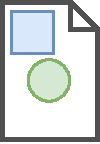
\includegraphics[scale=0.5]{collab/doc-a1-b1.pdf}}},
                label={[shift={(-0.1,-0.7)}]left:{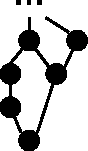
\includegraphics[scale=0.5]{fig/collab/log-sample.pdf}}}
            ](A){
\includegraphics[scale=0.6]{collab/device.pdf}}
            to +(70:2) node[
                label=above:{Bea},
                label={[shift={(0,0.7)}]right:{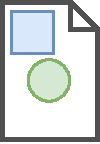
\includegraphics[scale=0.5]{collab/doc-a1-b1.pdf}}},
                label={[shift={(0.1,-0.7)}]right:{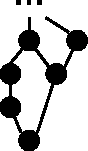
\includegraphics[scale=0.5]{fig/collab/log-sample.pdf}}}
            ](B){
\includegraphics[scale=0.6]{collab/device.pdf}}
            to +(-50:2) node[
                label=below:{Carol}
            ](C){
\includegraphics[scale=0.6]{collab/device.pdf}};
        % Links
        \draw (A) edge[link] (B);
        \draw (B) edge[link] (C);
        \draw (A) edge[link,-latex] node[midway]{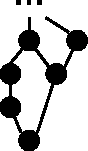
\includegraphics[scale=0.5]{fig/collab/log-sample.pdf}} (C);
    \end{tikzpicture}
    \caption{}\label{fig:invite-by-log-1}
\end{subfigure}
\begin{subfigure}{0.49\linewidth}
\centering
    \begin{tikzpicture}
        % devices
        \path (0,0)
            to +(190:2) node[
                label=below:{Alice},
                label={[shift={(0,0.7)}]left:{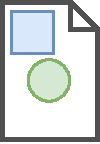
\includegraphics[scale=0.5]{collab/doc-a1-b1.pdf}}},
                label={[shift={(-0.1,-0.7)}]left:{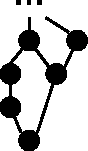
\includegraphics[scale=0.5]{fig/collab/log-sample.pdf}}}
            ](A){
\includegraphics[scale=0.6]{collab/device.pdf}}
            to +(70:2) node[
                label=above:{Bea},
                label={[shift={(0,0.7)}]right:{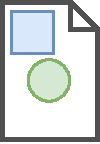
\includegraphics[scale=0.5]{collab/doc-a1-b1.pdf}}},
                label={[shift={(0.1,-0.7)}]right:{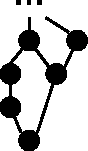
\includegraphics[scale=0.5]{fig/collab/log-sample.pdf}}}
            ](B){
\includegraphics[scale=0.6]{collab/device.pdf}}
            to +(-50:2) node[
                label=below:{Carol},
                label={[shift={(0,0.7)}]right:{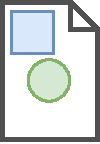
\includegraphics[scale=0.5]{collab/doc-a1-b1.pdf}}},
                label={[shift={(0.1,-0.7)}]right:{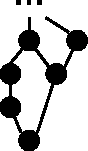
\includegraphics[scale=0.5]{fig/collab/log-sample.pdf}}}
            ](C){
\includegraphics[scale=0.6]{collab/device.pdf}};
        % Links
        \draw[link] (A) to (B);
        \draw[link] (B) to (C);
        \draw[link] (C) to (A);
    \end{tikzpicture}
    \caption{}\label{fig:invite-by-log-2}
\end{subfigure}
\caption[Transmission d'un journal complet à une nouvelle collaboratrice]{Alice et Bea répliquent de manière optimiste un dessin.
Ils utilisent un journal infalsifiable pour assurer la convergence des copies des pairs honnêtes.
Carol veut rejoindre la collaboration.
\subref{fig:invite-by-log-1} Alice envoie son journal à Carol.
\subref{fig:invite-by-log-2} Carol vérifie l'authenticité du journal et construit le dessin à partir du journal.}\label{fig:invite-by-log}
\end{figure}

Les pairs doivent préserver l'intégralité de leur journal pour \begin{inlinelist}
\item détecter les équivoques et
\item permettre à un pair de rejoindre la collaboration
\end{inlinelist}.
Un pair qui rejoint la collaboration a en effet besoin du journal pour obtenir l'état actuel du contenu partagé.
Il obtient cet état en intégrant sur sa copie vierge du contenu partagé chaque modification enregistrée dans le journal.
La \autoref{fig:invite-by-log} illustre la transmission d'un journal infalsifiable à un pair qui rejoint la collaboration.
La préservation de l'intégralité du journal engendre plusieurs problèmes~:

\paragraph{Passage à l'échelle.} Au fur et à mesure de la progression de la collaboration, les journaux contiennent de plus en plus de modifications.
La préservation de l'intégralité d'ub journal et leur transmission aux pairs qui rejoignent la collaboration sont donc de plus en plus coûteuses.

\paragraph{Vie Privée.} La préservation du journal dans son intégralité expose l'historique de la collaboration depuis son commencement.
Bien que certaines applications requièrent cette historique pour fournir des fonctionnalités, telle que la visualisation interactive de l'évolution d'un contenu, il peut être intéressant d'offrir plus de liberté sur quelles données doivent être conservées et quelles données doivent être supprimées.

\paragraph{} Pour répondre à ces deux problématiques nous effectuons deux observations~:
\begin{itemize}
    \item Toutes les modifications ne sont pas forcément nécessaires à la détection d'équivoques.
    \item L'occupation mémoire de la copie du contenu partagé est généralement plus fiable que celle du journal.
\end{itemize}

Nous proposons ainsi deux mécanismes~:

\paragraph{Troncature du journal.} Au lieu de préserver l'intégralité du journal, seules les modifications nécessaires à la détection d'équivoques pourraient être conservées.
Pour supprimer une modification du journal nous devons nous assurer qu'elle n'est pas nécessaire à la détection des équivoques futures.
Pour ce faire, nous utilisons des journaux infalsifiables dans lesquels chaque modification déclare des dépendances sur d'autres modifications.
Les dépendances sont déclarées de telle manière à résister aux équivoques.
En d'autres termes, si un pair mal-intentionné effectue une équivoque en générant deux modifications $x$ et $y$ et qu'une modification $z$ déclare dépendre de $x$, alors nous considérons qu'il n'est pas possible de prétendre que $z$ dépend de $y$.
Les modifications et leurs dépendances forment ainsi un graphe dirigé sans cycle.
Nous contraignons l'acceptation de modifications dans un journal de telle manière à ce que les modifications acceptées ultérieurement partagent un ensemble croissant de dépendances.
Nous déterminons cet ensemble à l'aide du concept de \emph{stabilité}.
Au sein d'un journal, une modification devient \emph{stable} une fois que toutes les modifications acceptées ultérieurement dans le journal dépendent de cette modification.
Nous proposons un protocole qui permet de supprimer un sous-ensemble des modifications stables.
Lorsque des modifications sont supprimées du journal nous disons que le journal est \emph{tronqué}.
La \autoref{fig:log-example} donne un exemple d'un journal et d'une version tronquée de ce journal.

\begin{figure}[hbt]
\centering
\begin{tikzpicture}
    \newcommand*\hsep{2}
    \path node (a1) {$a_1$}
        to +(\hsep,0) node (a2) {$a_2$}
        to +(2*\hsep,0) node (b1) {$b_1$}
        to +(3*\hsep,0) node (a3) {$a_3$}
        to +(4*\hsep,0) node (b2) {$b_2$}
        to +(5*\hsep,0) node (a4) {$a_4$}
    ;
    % Dependency
    \foreach \src/\dest in {a1/a2,b1/a3,a3/b2}
        \draw[pre] (\src) to (\dest);
    \draw[pre] (b2) to coordinate(b2a4) (a4);
    \draw[pre,bend right=30] (a1) to (b1);
    \draw[pre,bend left=30] (a2) to (a3);
    % pruned
    \node[draw,dashed,fit=(b2) (b2a4) (a4)]{};
\end{tikzpicture}
\caption[Exemple du journal d'un pair]{Exemple du journal d'un pair.
L'arrangement horizontal des opérations traduit leur ordre d'ajout dans le journal.
Ainsi les opérations ont été ajoutées dans l'ordre suivant~: $a_1$, $a_2$, $b_1$, $a_3$, $b_2$, $a_4$.
Un arc dirigé entre deux modifications se traduit par \enquote{est une dépendance déclarée de}.
La partie entourée correspond à une version tronquée de ce journal.
}\label{fig:log-example}
\end{figure}

\paragraph{Transmission d'un état authentifiable.} Au lieu de récupérer un journal dans son intégralité, un pair qui rejoint une collaboration pourrait récupérer l'état actuel d'une copie du contenu partagé.
Un pair mal-intentionné peut construire un état de toutes pièces avant de le transmettre à un pair qui rejoint la collaboration.
Le nouveau pair n'a aucun moyen de décider si l'état qu'il reçoit est authentique ou falsifié.
Pour s'assurer de l'authenticité d'un état nous proposons un protocole qui permet d'authentifier un état à partir d'un journal tronqué.
Lorsqu'un pair rejoint la collaboration il récupère un état ainsi que le journal tronqué qui lui est associé.
La \autoref{fig:invite-by-snaplog} illustre cette approche.

\paragraph{} Nous développons d'abord le concept de stabilité dans la \autoref{sec:stability}.
Dans la \autoref{sec:full-log-protocol}, nous présentons un protocole qui protége la convergence des copies à l'aide de journaux intégrales.
Nous nous basons sur ce protocole pour présenter dans la \autoref{sec:pruned-log-protocol} un protocole qui permet de tronquer un journal et d'authentifier un état à partir d'un journal tronqué.

\begin{figure}[htb]
\centering
\begin{subfigure}{0.49\linewidth}
    \centering
    \begin{tikzpicture}
        % devices
        \path (0,0)
            to +(190:2) node[
                label=below:{Alice},
                label={[shift={(0,0.7)}]left:{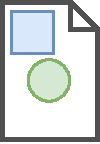
\includegraphics[scale=0.5]{collab/doc-a1-b1.pdf}}},
                label={[shift={(-0.1,-0.7)}]left:{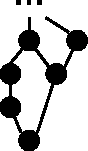
\includegraphics[scale=0.5]{fig/collab/log-sample.pdf}}}
            ](A){
\includegraphics[scale=0.6]{collab/device.pdf}}
            to +(70:2) node[
                label=above:{Bea},
                label={[shift={(0,0.7)}]right:{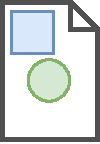
\includegraphics[scale=0.5]{collab/doc-a1-b1.pdf}}},
                label={[shift={(0.1,-0.7)}]right:{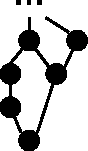
\includegraphics[scale=0.5]{fig/collab/log-sample.pdf}}}
            ](B){
\includegraphics[scale=0.6]{collab/device.pdf}}
            to +(-50:2) node[
                label=below:{Carol}
            ](C){
\includegraphics[scale=0.6]{collab/device.pdf}};
        % Links
        \draw (A) edge[link] (B);
        \draw (B) edge[link] (C);
        \draw (A) edge[link,-latex] node[midway,below]{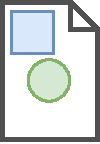
\includegraphics[scale=0.5]{collab/doc-a1-b1.pdf}} node[midway,above]{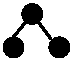
\includegraphics[scale=0.5]{fig/collab/pruned-log.pdf}} (C);
    \end{tikzpicture}
    \caption{}\label{fig:invite-by-snaplog-1}
\end{subfigure}
\begin{subfigure}{0.49\linewidth}
\centering
    \begin{tikzpicture}
        % devices
        \path (0,0)
            to +(190:2) node[
                label=below:{Alice},
                label={[shift={(0,0.7)}]left:{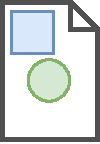
\includegraphics[scale=0.5]{collab/doc-a1-b1.pdf}}},
                label={[shift={(-0.1,-0.7)}]left:{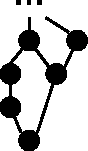
\includegraphics[scale=0.5]{fig/collab/log-sample.pdf}}}
            ](A){
\includegraphics[scale=0.6]{collab/device.pdf}}
            to +(70:2) node[
                label=above:{Bea},
                label={[shift={(0,0.7)}]right:{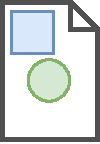
\includegraphics[scale=0.5]{collab/doc-a1-b1.pdf}}},
                label={[shift={(0.1,-0.7)}]right:{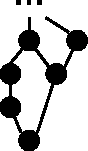
\includegraphics[scale=0.5]{fig/collab/log-sample.pdf}}}
            ](B){
\includegraphics[scale=0.6]{collab/device.pdf}}
            to +(-50:2) node[
                label=below:{Carol},
                label={[shift={(0,0.5)}]right:{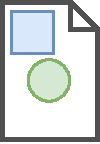
\includegraphics[scale=0.5]{collab/doc-a1-b1.pdf}}},
                label={[shift={(0.2,-0.5)}]right:{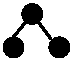
\includegraphics[scale=0.5]{fig/collab/pruned-log.pdf}}}
            ](C){
\includegraphics[scale=0.6]{collab/device.pdf}};
        % Links
        \draw (A) edge[link] (B);
        \draw (B) edge[link] (C);
        \draw (C) edge[link] (A);
    \end{tikzpicture}
    \caption{}\label{fig:invite-by-snaplog-2}
\end{subfigure}
\caption[Transmission d'un journal tronqué et d'un état à une nouvelle collaboratrice]{Alice et Bea répliquent de manière optimiste un dessin.
Ils utilisent un journal infalsifiable pour assurer la convergence des copies des pairs honnêtes.
Carol veut rejoindre la collaboration.
\subref{fig:invite-by-log-1} Alice envoie l'état actuel de sa copie du dessin, ainsi qu'une version tronquée de son journal infalsifiable.
\subref{fig:invite-by-log-2} Carol vérifie l'authenticité du journal tronqué.
Elle vérifie également l'authenticité de l'état reçu à partir du journal tronqué.}\label{fig:invite-by-snaplog}
\end{figure}



% Une manière de réduire ce coût est de conserver seulement les opérations les plus récentes.
% Ces opérations forment un suffixe du journal original.
% Nous disons que le journal est tronqué.
% La troncature du journal permet à l'adversaire de la collaboration de mener de nouvelles attaques en vue de faire diverger les copies des pairs honnêtes.
% La suppression de modification du journal peut en effet compromettre la détection d'équivoques.
% Pouvons-nous concevoir un protocole qui permet la troncature du journal sans compromettre la convergence des copies~?

% Une observation importante est que toutes les modifications ne sont pas nécessaires à la détection des équivoques et au maintien de la cohérence du journal.
% En posant des contraintes sur l'acceptation des modifications dans le journal nous pouvons construire un préfixe croissant de modifications du journal qui ne sont plus nécessaires au maintien de la cohérence du journal et à la détection d'équivoques.

% La suppression de modifications du journal se base sur le concept de stabilité que nous développons dans la \autoref{sec:stability}.
% La \autoref{sec:protocole-overview} donne un aperçu du protocole à journaux tronqué que nous présentons dans la \autoref{sec:full-log-protocol} et la \autoref{sec:pruned-log-protocol}.

%Un pair honnête ne peut pas tronquer son journal de manière arbitraire sans menacer la cohérence future de son journal ou la convergence de son journal avec journaux des autres pairs honnêtes.
%La cohérence d'un journal est conservée en vérifiant systématiquement les opérations qui sont reçues.

%Un journal ne peut être arbitrairement tronqué sans menacer la cohérence future du journal ou sa convergence avec les autres journaux.
%Une opération est ajoutée dans un journal cohérent, si elle ne rend pas ce dernier incohérent.
%Cette vérification requiert la présence d'un certain nombre d'opérations qui dépendent du modèle de cohérence considéré.
%Par exemple, pour vérifier une opération dans un journal qui respecte le modèle de cohérence PRAM (ou FIFO), seule l'opération précédente du même auteur est requise.
%Si des opérations nécessaires à la vérification d'une opération sont manquantes, l'opération ne peut être vérifiée.
%L'opération doit donc être rejetée ou intégrée dans le journal avec le risque de le rendre incohérent.
%Pour conserver un journal cohérent, le rejet semble donc le choix le plus judicieux.
%Cependant, elle peut conduire à une divergence permanente des journaux.
%Certains journaux peuvent avoir vérifié et intégré des opérations, e d'autres peuvent les avoir rejetées parce qu'elles ne peuvent pas être vérifiées.
%
%Afin de maintenir un journal cohérent et convergent, les pairs doivent conserver les opérations nécessaires à la vérification de toutes nouvelles opérations.
%Pour supprimer des opérations nous devons donc rencontrer deux conditions~: les opérations nécessaires à la vérification d'une opération devraient représenter un sous-ensemble du journal, et la collaboration devrait progresser de telle manière qu'un préfixe croissant d'opérations n'est plus nécessaire pour vérifier toutes nouvelles opérations.
%Ces deux contraintes peuvent être atteintes en utilisant un modèle de cohérence.
%Un modèle de cohérence restreint la manière dont peuvent être mises en relation deux opérations.
%La concurrence entre opérations joue un rôle important dans la détermination des opérations qui peuvent être ôtées du journal.
%Nous disons qu'une opération est stable une fois qu'il n'est plus possible d'intégrer dans le journal une opération qui lui est concurrente.
%
%Dans un premier temps nous explorons la stabilisation de journaux de manière itératif. dans un second temps, nous utilisant la notion de stabilité pour définir qu'elle partie d'un journal peut être tronquée sans menacer sa cohérence future ou sa convergence avec les autres journaux.


% \section{Aperçu}\label{sec:protocole-overview}

% La convergence à terme des copies est une propriété essentielle des infrastructures pair-à-pair de collaboration.
% Des pairs mal-intentionnés peuvent trouver un intérêt à compromettre la convergence des copies des pairs honnêtes.
% Pour empêcher de tels scénarios, les pairs honnêtes peuvent maintenir un journal infalsifiable et répliqué.
% Ils enregistrent l'ensemble de leurs modifications dans leur journal respectif.
% Les pairs synchronisent leurs journaux afin de récupérer et intégrer sur leur copie les modifications de chacun.

% Chaque pair doit conserver l'intégralité de son journal pour \begin{inlinelist}
%     \item vérifier la cohérence du journal lors de l'ajout d'une nouvelle opération
%     \item permettre à de nouveaux pairs de rejoindre la collaboration
% \end{inlinelist}.
% Les nouveaux pairs jouent les opérations enregistrées dans le journal pour obtenir le document partagé.
% La \autoref{fig:invite-by-log} montre que les nouveaux pairs utilisent le journal pour obtenir le document partagé.
% Pour ce faire, ils intègrent les modifications enregistrées dans le journal.
% La préservation de l'intégralité du journal engendre plusieurs problèmes~:

% \paragraph{Passage à l'échelle.} Au fur et à mesure de la progression de la collaboration les journaux contiennent de plus en plus d'entrées.
% La préservation des journaux et leur transmission aux pairs qui rejoignent la collaboration sont donc de plus en plus coûteuses.

% \paragraph{Vie Privée.} La préservation du journal dans son intégralité expose l'historique de la collaboration depuis son commencement.
% Bien que certaines applications requièrent cette historique pour fournir des fonctionnalités, telle que la visualisation interactive de l'évolution d'un document, il peut être intéressant d'offrir plus de liberté sur quelles données doivent être conservées et quelles données doivent être supprimées.

% \bigskip

% Un journal enregistre l'ensemble des modifications qui ont été intégrées à un contenu partagé.
% Un contenu est souvent plus petit que le journal qui lui est attaché.
% Certaines applications prennent avantage de cette observation.
% Au lieu de transmettre un journal à un nouveau pair, elles transmettent un instantané du document.

% Notre contexte ne nous permet pas d'adopter cette approche.
% En effet, un pair mal-intentionné peut facilement falsifier un instantané du document avant de la transmettre à un nouveau pair.
% Ce dernier n'a aucun moyen de vérifier l'authenticité de l'instantané.

% Nous proposons une approche qui permet de tronquer le journal infalsifiable et d'authentifier un instantané à partir du journal tronqué qui lui est associé.
% La \autoref{fig:invite-by-snaplog} illustre cette approche.

% Un journal ne peut pas être tronqué de manière arbitraire.
% Un pair doit conserver suffisamment d'opérations pour maintenir la cohérence de son journal.
% Avant d'ajouter une opération dans son journal, il vérifie que l'ajout de cette dernière ne compromet pas la cohérence de son journal.
% Au cours de la collaboration, un sous-ensemble croissant d'opérations du journal ne devraient plus être nécessaires à la vérification de la cohérence du journal.
% Ces opérations peuvent alors être supprimées du journal.

% Nous considérons des journaux dans lesquels les opérations ont des relations de dépendance.
% Un journal forme ainsi un graphe dirigé sans cycle.
% La \autoref{fig:log-example} donne un exemple d'un journal.
% Pour former ce sous-ensemble croissant d'opérations supprimables, les opérations futures devraient partager un préfixe commun de dépendances qui croît de manière monotone au cours de la collaboration.
% Par exemple, dans la \autoref{fig:log-example}, si nous savons que toutes les opérations futures dépendent sur l'opération $a_4$ et que $a_4$ est suffisante à la vérification future de la cohérence du journal, alors les opérations qui précédent $a_4$ peuvent être supprimées du journal.

% \begin{figure}[hbt]
% \centering
% \begin{tikzpicture}
%     \newcommand*\hsep{1.5}
%     \newcommand*\vsep{-1.2}
%     % Peers
%     \path node (A) {$p_A$}
%         to +(0,\vsep) node (B) {$p_B$}
%     ;
%     % Events
%     \path (A)
%         to +(\hsep,0) node (a1) {$a_1$}
%         to +(2*\hsep,0) node (a2) {$a_2$}
%         to +(4*\hsep,0) node (a3) {$a_3$}
%         to +(5*\hsep,0) node (a4) {$a_4$}
%     ;
%     \path (B)
%         to +(3*\hsep,0) node (b1) {$b_1$}
%         to +(6*\hsep,0) node (b2) {$\top_{\trm{vis}}$}
%     ;
%     % Timelines
%     \path (6.5*\hsep,0) coordinate (aend)
%         to +(0,\vsep) coordinate (bend)
%     ;
%     \foreach \src/\dest in {A/a1,B/b1,b1/b2,a4/aend,b2/bend}
%         \draw[timeline] (\src) to (\dest);
%     % Visibility
%     \foreach \src/\dest in {a1/a2,a2/a3,a3/a4,a2/b1,b1/a4,a4/b2}
%         \draw[pre] (\src) to (\dest);
% \end{tikzpicture}
% \caption[Représentation d'un journal]{Exemple d'un journal.
% L'arrangement horizontal des opérations traduit leur ordre d'ajout dans le journal.
% Ainsi les opérations ont été ajoutées dans l'ordre suivant~: $a_1$, $a_2$, $b_1$, $a_3$, $a_4$.
% L'opération $\top_{\trm{vis}}$ est un peu particulière.
% Son auteur $p_B$ correspond au possesseur du journal.
% Les arcs dirigés mettent en évidence les dépendances immédiates des opérations.
% Par exemple, $a_2$ est une dépendance immédiate de $a_3$ et $b_1$.
% }\label{fig:log-example}
% \end{figure}

% Lorsqu'une opération est une dépendance de toutes opérations futures, nous disons que cette opération est stable.
% Un journal est stabilisable lorsqu'il a un préfixe d'opérations stable qui peut croître au cours de la collaboration.
% Pour ce faire, nous devons contraindre l'acceptation des opérations au sein d'un journal de telle manière à ce qu'une opération soit stable une fois qu'un certain nombre de conditions sont rencontrées.

% Dans la \autoref{sec:stability} nous développons le concept de stabilité et nous recherchons un modèle de cohérence stabilisable en présence de pairs mal-intentionnés.

%\section{Journaux}
%
%Chaque pair honnête maintient une copie d'un type répliqué $T$.
%Les pairs synchronisent l'état de leurs copies en échangeant leurs modifications.
%
%Chaque pair honnête possède un journal dans lequel il enregistre l'ensemble des opérations qu'il intègre à sa copie.
%Il s'agit des opérations qu'il transmet aux autres pairs et aux opérations qu'il accepte des autres pairs.
%Une opération intégrée $x$ est caractérisée par~:
%\begin{itemize}
%    \item un identifiant globalement unique $\trm{id}(x)$
%    \item le pair qui est à son origine $\trm{peer}(x)$
%    \item l'appel qui a été originellement effectué $\trm{call}(x)$
%    \item les identifiants de ses dépendances immédiates déclarées $\trm{deps}(x)$.
%\end{itemize}
%
%Un pair honnête intègre de manière séquentielle les opérations.
%Les opérations sont donc linéairement ordonnées par l'ordre dans lequel elles sont intégrées sur la copie et dans le journal.
%
%\begin{definition}[Journal]
%Un \emph{journal} d'un contenu répliqué de type $T$ est un n-uplet $J \defeq \tuple*{E, \trm{owner}, \trm{ao}}$ tel que~·
%\begin{itemize}
%\item $E$ est un ensemble dénombrable d'opérations intégrées
%\item $\trm{owner} \in \trm{Honest}$ est le pair honnête qui possède le journal
%\item $\trm{ao} \subseteq J \times J$ est l'ordre dans lequel les opérations sont ajoutées dans le journal (\emph{acceptation-order}).
%Il s'agit d'un ordre total strict localement fini.
%\end{itemize}
%\end{definition}
%
%Lorsqu'un pair déclare des dépendances sur l'une de ses opérations, cette dernière dépend récursivement sur les dépendances de ses dépendances.
%Nous pouvons ainsi définir la relation suivante~:
%
%\paragraph{Dépendance.} Une relation qui rend compte des dépendances transitives entre les opérations d'un journal.
%Une opération $x$ est une dépendance d'une opération $z$, et nous écrivons $x \dep z$, si et seulement si $x$ est une dépendance déclarée de $z$ ou il existe une dépendance $y$ de $z$ tel que $x$ est une dépendance de $y$.
%\begin{equation*}
%    x \dep z \defiff \trm{id}(x) \in \trm{deps}(z) \lor \exists y \qsep x \dep y \dep z
%\end{equation*}
%
%\begin{definition}[Journal bien-formé]
%Un \emph{journal} est bien-formé si et seulement si la relation de dépendance est un ordre partiel localement fini.
%\end{definition}
%
%\begin{definition}[Journal complet]
%Un journal $J$ est \emph{complet} si et seulement si chaque dépendance déclarée de chaque opération est présente dans $J$.
%\begin{equation*}
%    J \textit{complet} \defiff \:\forall y \in J \:\forall k \in \trm{deps}(y) \:\exists x \in J \qsep \trm{id}(x) = k
%\end{equation*}
%\end{definition}
%
%%Lorsqu'un pair enregistre une de ses propres opérations dans son journal, il s'assure que chaque opération présente dans le journal est une dépendance de l'opération qu'il enregistre.
%%Nous disons que le journal est bien-formé.
%%
%%\begin{definition}[Journal bien-formé]
%%Un \emph{journal} $J$ est bien-formé si et seulement si chaque opération du possesseur du journal a pour dépendance l'ensemble des opération du journal qui précède son ajout.
%%\begin{equation*}
%%    \forall y \in J \qsep \trm{peer}(y) = \trm{owner} \implies \forall x \ao y \qsep x \dep y
%%\end{equation*}
%%\end{definition}
%
%\begin{remark}
%Dans la suite de ce manuscrit nous considérons uniquement des journaux bien-formés.
%\end{remark}
%
%Les pairs s'assurent que les dépendances déclarée d'une opération sont présente dans le journal avant d'intégrer cette dernière à leur copie et à leur journal.
%
%Les pairs maintiennent des journaux cohérents.
%Lorsqu'ils ajoutent une nouvelle opération dans leur journal, ils vérifient que cette dernière ne compromet pas la cohérence de leur journal.
%Les garanties de cohérence auxquelles nous nous intéressons concernent principalement des restrictions d'ordre sur les relations de dépendance entre les opérations.
%Au lieu de partir de zéro, nous pouvons nous rattacher aux concepts introduits dans le \autoref{ch:background}.
%Pour ce faire, il nous suffit de créer une correspondance entre un journal et une exécution abstraite.
%Nous parlons d'exécution abstraite associée à un journal.
%
%Une exécution abstraite rend compte de l'observation de chaque pair honnête.
%En déclarant une dépendance sur l'une de ses opérations, un pair honnête atteste avoir observée (et intégrée) la dépendance avant l'exécution de l'opération considérée.
%Les relations de dépendances entre opérations exposent donc les observations des pairs honnêtes.
%Nous pouvons donc créer une correspondance entre les relations de dépendance au sein d'un journal et les relations de \emph{visibilité} au sein de l'exécution abstraite associée au journal.
%
%Les dépendances déclarées par les pair mal-intentionnées ne traduisent pas nécessairement leurs observations réelles.
%Il en va de même au sein d'une exécution abstraite~: les relations de \emph{visibilité} ne traduisent pas les observations des pairs mal-intentionnées.
%
%Cette correspondance n'est pas suffisante.
%Lorsqu'un pair honnête ajoute une opération dans son journal, il l'observe.
%cette observation devrait être exposée au sein de l'exécution abstraite associée au journal.
%Pour ce faire, une exécution abstraite associée inclut une opération supplémentaire~: l'opération d'observation implicite.
%L'opération d'observation implicite a pour auteur le possesseur du journal et toutes les autres opérations lui sont visibles.
%
%Au lieu de présenter un nouveau formalisme graphique pour représenter un journal, nous représentons simplement l'exécution abstraite associée au journal.
%L'opération d'observation implicite permet d'identifier le possesseur du journal.
%La \autoref{fig:log-example} est une exécution abstraite qui représente le journal du pair $p_B$.
%$\top_{\trm{vis}}$ est l'opération d'observation implicite.
%Dans cet exemple nous utilisons la relation de précédence présentée dans la \autoref{subsec:caucal-consistency}.
%Dans une représentation graphique elle indique que la relation de visibilité est transitive.
%
%\begin{definition}[Exécution abstraite associée]
%Pour tout journal $J \defeq \tuple*{E, \trm{owner}, \trm{ao}}$, il existe une unique histoire associée $H \defeq \tuple*{E \cup \set*{\top_{\trm{vis}}}, \trm{peer}_H, \trm{call}_H, \trm{rval}, \trm{rb}}$ et une unique exécution abstraite associée $A \defeq \tuple*{H, \trm{vis}}$ tel que~:
%\begin{itemize}
%\item $\top_{\trm{vis}}$ est l'opération d'observation implicite.
%Elle est absente de $E$.
%L'auteur et l'appel d'une opération dans l'histoire $H$ est identique à l'auteur et à l'appel dans $E$.
%Nous définissons l'auteur et l'appel de l'opération d'observation implicite comme étant le possesseur du journal et l'opération sans effet $\trm{noop}$.
%\begin{align*}
%    &\trm{peer}_H(x) \defeq \begin{dcases}
%        \trm{peer}_E(x) & \when x \neq \top_{\trm{vis}}\\
%        \trm{owner} &
%    \end{dcases}
%    &\trm{call}_H(x) \defeq \begin{dcases}
%        \trm{call}_E(x) & \when x \neq \top_{\trm{vis}}\\
%        \trm{noop} &
%    \end{dcases}
%\end{align*}
%\item L'histoire $H$ n'inclut pas d'opérations d'interrogations.
%\begin{equation*}
%    \trm{rval} \defeq \emptyset
%\end{equation*}
%\item La relation \emph{retourne-avant} $\trm{rb}$ est construite à partir de l'ordre d'ajout des opérations dans le journal.
%Toute opération du journal retourne-avant l'opération d'observation implicite $\top_{\trm{vis}}$.
%\begin{equation*}
%    x \rb z \defiff x \ao z \lor z = \top_{\trm{vis}}
%\end{equation*}
%\item La relation de visibilité $\trm{vis}$ est construite à partir des relations de dépendance entre les opérations.
%Toutes opération de $H$ est visible à l'opération d'observation implicite $\top_{\trm{vis}}$.
%\begin{equation*}
%    x \vis z \defiff x \dep z \lor z = \top_{\trm{vis}}
%\end{equation*}
%\end{itemize}
%\end{definition}
%
%
%\begin{claim}\label{th:rb-linear-order}
%La relation \emph{retourne-avant} de l'exécution abstraite associée à un journal est une énumération.
%\end{claim}
%% A prouver?
%
%\begin{proposition}
%L'exécution abstraite associée d'un journal est bien-formée.
%\end{proposition}
%
%\begin{proof}
%Suivant l'\autoref{th:rb-linear-order}, nous déduisons que toute restriction de la relation \emph{retourne-avant} aux opérations d'un pair donné (mal-intentionné ou honnête) est une énumération.
%Par conséquent, la propriété~\ref{itm:bf1} est respectée.
%
%Toutes les opérations de $E$ sont visibles à l'opération d'observation implicite $\top_{\trm{vis}}$.
%L'auteur de cette dernière est le possesseur du journal.
%Il est par définition honnête.
%Par conséquent, toutes les opération, y compris les opérations émises par des pairs mal-intentionnées, sont observées par au moins un pair honnête.
%La propriété~\ref{itm:bf2} est donc satisfaite.
%\end{proof}
%
%
%\begin{definition}[Journal cohérent]
%Un journal respecte un modèle de cohérence $C$ si et seulement si son exécution abstraite associée respecte $C$.
%\end{definition}
%
%L'exécution abstraite de la \autoref{fig:log-example} respecte le modèle de cohérence causale.
%Le journal qui lui est associé respecte donc le modèle de cohérence causale.
%
%Dans le \autoref{ch:background}, nous utilisions les exécutions abstraite pour expliquer une exécution d'un point de vue global.
%Nous savions alors quels pairs sont honnêtes et lesquels sont mal-intentionnés.
%Une exécution abstraite associée à un journal décrit en revanche la connaissance qu'a le possesseur du journal sur l'exécution.
%Nous adoptons donc un point de vue d'un pair.
%Le pair ne sait pas si un pair donné est honnête ou mal-intentionné.
%Le pair pourrait faire confiance à un ensembles de pairs qu'il considère honnête.
%Nous préférons prendre une approche plus pessimiste : un pair honnête considère que tout autre pair est potentiellement mal-intentionné.
%
%\begin{remark}
%Dans une exécution abstraite associée à un journal, tous les pairs, à l'exception du possesseur du journal, sont considérés mal-intentionnés.
%Puisque nous définissons nos concepts sur les exécutions abstraites, nous pouvons facilement changer cette hypothèse.
%\end{remark}
%
%% Décrire un protocole à base de journaux répliqués ?
%
%Pour tronquer un journal nous avons besoin d'identifier quels opérations peuvent être su primées sans compromettre la cohérence du journal.
%Dans la section suivante nous introduisons le concept de stabilité qui nous approche de cet identification.
%

\section{Stabilité}\label{sec:stability}

\subsection{Généralités}\label{subsec:general-stability}

Dans la littérature~\autocite{baquero_2018_pure-op-crdt, shapiro_2011_crdt,birman_1991_causalmulticast}, la stabilité désigne souvent un prédicat qui une fois vrai le reste pour toujours.
Dans ce manuscrit, nous disons qu'une modification est stable au sein d'un journal lorsqu'elle devient une dépendance de toutes les modifications qui sont ultérieurement acceptées dans le journal.
Pour permettre la stabilisation de modifications, les pairs doivent accepter les modifications dans leur journal sous certaines conditions.
Par exemple, si toute modification est acceptée au sein d'un journal seulement si elle dépend de toutes les modifications déjà présentes dans le journal, alors toutes les modifications enregistrées dans le journal sont stables.
Les relations de dépendances forment un ordre total.
Notre objectif est de trouver des contraintes d'acceptation qui permettent à terme la stabilisation de toute modification et qui sont adaptées à la réplication optimiste et à la présence de pairs mal-intentionnés.

Au lieu de circonscrire nos contributions à des journaux, nous décrivons ces contraintes et le concept de stabilité dans un modèle plus général.
Pour éviter l'introduction d'un nouveau modèle, nous réutilisons le concept d'exécution abstraite définit dans le \autoref{ch:background}.
Une exécution abstraite est suffisamment générale pour représenter une exécution ou un journal.
Lorsqu'une exécution abstraite représente un journal, nous parlons d'exécution abstraite associée à un journal.
Nous détaillons dans la \autoref{sec:full-log-protocol} comment obtenir à partir d'un journal son exécution abstraite associée.
Pour simplifier la compréhension nous utilisons dans les exemples des exécutions abstraites qui ne sont pas forcément associées à des journaux.
Les contraintes d'acceptation d'une modification au sein d'un journal se traduisent par des propriétés de cohérence sur les opérations au sein d'une exécution abstraite.

% Nous recherchons un modèle de cohérence qui puisse être respecté par un protocole de réplication optimiste qui tolère la présence de pairs mal-intentionnés et permet la stabilisation d'opérations.
% Le modèle de cohérence doit donc être compatible avec le modèle de cohérence à terme forte.
% Il doit permettre aux pairs honnêtes de toujours exécuter une opération.

Pour définir la stabilité au sein d'une exécution abstraite, la \autoref{def:abstract-exec-extension} introduit le concept d'extension d'une exécution abstraite.
Cette définition repose sur le concept d'extension d'une histoire introduit dans la \autoref{subsec:consistency-spec-liveness-safety} du \autoref{ch:background}.

\begin{definition}[Extension d'une exécution abstraite]\label{def:abstract-exec-extension}
Une exécution abstraite $A' \defeq \tuple*{H',\trm{vis}'}$ est une extension d'une exécution abstraite (bien-formée ou mal-formée) $A \defeq \tuple*{H,\trm{vis}}$, et nous écrivons $A' \sqsupset A$, si et seulement si~:
\begin{itemize}
    \item L'histoire $H'$ de $A'$ est une extension de l'histoire $H$ de $A$~:

    \begin{equation*}
    H' \sqsupset H
    \end{equation*}

    \item Les relations de visibilité sont inchangées.

    \begin{equation*}
    x, y \in A \land x \vis_{A'} y \iff x \vis_{A} y
    \end{equation*}
\end{itemize}
\end{definition}

% \begin{definition}[Extension cohérente]\label{def:consistent-extension}
% Si une extension $A'$ d'une exécution abstraite (bien-formée ou mal-formée) $A$ respecte le modèle de cohérence $C$, alors par souci de concision nous écrivons $A' \sqsupset_C A$.
% $A$ ne respecte pas nécessairement le modèle de cohérence $C$.
% \begin{equation*}
% A' \sqsupset_C A \defiff A' \sqsupset A \land A' \in C
% \end{equation*}
% \end{definition}

Dans une exécution abstraite, une opération est stable une fois qu'elle est visible à toute opération future.
Puisque l’acceptation d’une opération est conditionnée par le modèle de cohérence, la stabilité l'est également.
Une opération peut être stable pour un modèle de cohérence donné et ne pas l'être pour un autre.
La \autoref{def:stable} définit formellement la stabilité.
Le \autoref{th:stability-hierarchy} met en perspective le concept de stabilité et de force d'un modèle de cohérence.

\begin{definition}[Opération stable]\label{def:stable}
Soit une opération $x$ d'une exécution abstraite (bien-formée ou mal-formée) $A$ qui respecte un modèle de cohérence $C$.
$x$ est $C$-stable dans $A$, et nous écrivons $\trm{stable}_A^C(x)$, si et seulement si il n'existe pas une opération $y$ d'une extension $A'$ de $A$ tel que $A'$ respecte $C$, $y$ est absente de $A$, et $x$ n'est pas visible à $y$.
\begin{equation*}
  \trm{stable}_A^C(x) \defiff \forall A' \sqsupset A \qsep A' \in C \implies \forall y \in A' \sminus A \qsep x \vis y
\end{equation*}
\end{definition}


\begin{theorem}\label{th:stability-hierarchy}
Soit deux modèles de cohérence $C$ et $C'$ tel que $C$ est plus fort que $C'$.
Si une opération d'une exécution abstraite $A$ est $C'$-stable, alors elle est également $C$-stable.
\begin{equation*}
    C \subset C' \land \trm{stable}_A^{C'}(x) \implies \trm{stable}_A^{C}(x)
\end{equation*}
\end{theorem}

\begin{proof}
Procédons par contradiction.
Soit deux modèles de cohérence $C$ et $C'$ tel que $C$ est plus fort que $C'$.
Soit une exécution abstraite $A$ qui respecte le modèle de cohérence $C$.
Elle respecte donc également le modèle de cohérence $C'$.
Supposons qu'il existe une opération $x$ de $A$ qui est $C'$-stable et n'est pas $C$-stable.
Puisque $x$ n'est pas $C$-stable, il existe donc une opération $y$ d'une extension $A'$ de $A$ tel que $A'$ respecte $C$, $y$ est absente de $A$, et $x$ n'est pas visible à $y$.
$A'$ respecte également $C'$.
$x$ n'est donc pas $C'$-stable.
Ce qui contredit l'hypothèse initiale.
\end{proof}

Nous souhaitons qu'au cours de l'exécution un ensemble croissant d'opérations deviennent stables.
En d'autres termes, toute opération devrait à terme devenir stable.
La \autoref{def:stabilisable} exprime cette attente sous la forme d'une propriété de vivacité.

\begin{definition}[Opération stabilisable]\label{def:stabilisable}
Soit une opération $x$ d'une exécution abstraite $A$ qui respecte un modèle de cohérence $C$.
$x$ est $C$-stabilisable dans $A$ si et seulement si il existe une extension de $A$ dans laquelle $x$ est $C$-stable.
$A$ garantit la propriété de vivacité $\trm{Stabilisable}_C$ si et seulement si toute opération de $A$ est $C$-stabilisable.
Un modèle de cohérence $C$ est stabilisable, et nous écrivons $C \in \trm{Stabilisable}$, si et seulement si toutes opérations de toutes les exécutions abstraites correctes et finies de $C$ sont $C$-stabilisables.
\begin{align*}
    A \in \trm{Stabilisable}_C &\defiff \forall x \in A \:\exists A' \sqsupset A \qsep A' \in C \land \trm{stable}_{A'}^C(x)\\
    C \in \trm{Stabilisable} &\defiff \forall A \in C \qsep A \textit{est finie} \implies A \in \trm{Stabilisable}_C
\end{align*}
\end{definition}
% TODO: vérifier si on peut remplacer \sqsupset par \sqsupseteq_C

Nous recherchons un modèle de cohérence stabilisable qui est réaliste dans le contexte de notre travail~: il doit garantir la disponibilité en lecture et en écritures des copies, ainsi que la convergence à terme des copies en présence de pairs mal-intentionnés.
Nous proposons d'abord d'explorer la notion de stabilité dans le modèle de cohérence causale et le modèle de cohérence \acl{VFJC}.
Ces deux modèles sont présentés dans le \autoref{ch:background}.
Nous construisons ensuite de nouveaux modèles de cohérence qui sont stabilisables et adaptés à notre contexte.


\clearpage % better layout

\subsection{Stabilité causale}\label{subsec:cs}

\textcite{baquero_2018_pure-op-crdt} ont introduit la stabilité causale comme un moyen de réduire la taille d'un journal.
La stabilité causale permet de supprimer les méta-données des opérations qui ne sont plus nécessaires au maintien de la cohérence de la copie et du journal d'un pair.
Leurs journaux respectent une variante du modèle de cohérence causale qui ne correspond pas exactement à celle introduite dans ce manuscrit.
%Le maintien de la cohérence d'un journal nécessite la connaissance des dépendances des opérations.
Ils remarquent que la connaissance des dépendances d'une opération n'est plus nécessaire une fois que toute opération reçue ultérieurement dépend de cette opération.

Leur définition de la stabilité causale se place du point de vue d'un pair.
Dans ce manuscrit, nous avons défini la stabilité sur une exécution abstraite.
Cette abstraction nous permet de raisonner autant d'un point de vue global, lorsque l'exécution abstraite explique une exécution, que d'un point de vue d'un pair, lorsque l'exécution abstraite est associée à un journal.

Pour définir la stabilité causale nous devons nous demander quand est-ce qu'une opération devient nécessairement visible à toute opération future.
Cette question revient à se demander quand est-ce qu'une opération ne peut plus être en concurrence avec une opération future.

Le modèle de cohérence causale contraint chaque pair à observer ses anciennes opérations.
Une opération d'un pair est donc nécessairement visible à toute opération future de ce même pair.
Par exemple, l'opération $a_1$ de la \autoref{fig:cs-example-1} sera visible aux opérations futures de son auteur $p_A$.
En se basant sur cette contrainte et la transitivité de la visibilité, nous déduisons qu'une fois qu'une opération quelconque est visible à l'opération d'un pair, elle l'est également à toute opération future de ce même pair.
Dans la \autoref{fig:cs-example-1}, $a_1$ est visible à l'opération $b_1$.
Puisque $b_1$ est visible à toute opération future de $p_B$, $a_1$ l'est également par transitivité.
Pour qu'une opération soit causalement stable, il suffit donc que chaque pair observe cette dernière.
Le \autoref{th:cs} définit formellement la stabilité causale.

\begin{figure}[htb]
\centering
\begin{subfigure}{.5\linewidth}
\centering
\begin{tikzpicture}
    \newcommand*\hsep{1.5}
    \newcommand*\vsep{-1.2}
    % Peers
    \path node (A) {$p_A$}
        to +(0,\vsep) node (B) {$p_B$}
        to +(0,2*\vsep) node (C) {$p_C$}
    ;
    % Events
    \path (A)
        to +(\hsep,0) node[stable,label={below:\scriptsize cs}] (a1) {$a_1$}
    ;
    \path (B)
        to +(2*\hsep,0) node (b1) {$b_1$}
    ;
    \path (C)
        to +(\hsep,0) node (c1) {$c_1$}
        to +(3*\hsep,0) node (c2) {$c_2$}
    ;
    % Timelines
    \path (3.5*\hsep,0) coordinate (aend)
        to +(0,\vsep) coordinate (bend)
        to +(0,2*\vsep) coordinate (cend)
    ;
    \foreach \src/\dest in {A/a1,B/b1,C/c1,a1/aend,b1/bend,c1/c2,c2/cend}
        \draw[timeline] (\src) to (\dest);
    % Precedence
    \foreach \src/\dest in {a1/b1,c1/b1,b1/c2}
        \draw[vis] (\src) to (\dest);
\end{tikzpicture}
\caption{}\label{fig:cs-example-1}
\end{subfigure}%
\begin{subfigure}{.5\linewidth}
\centering
\begin{tikzpicture}
    \newcommand*\hsep{1.5}
    \newcommand*\vsep{-1.2}
    % Peers
    \path node (A) {$p_A$}
        to +(0,\vsep) node (B) {$p_B$}
        to +(0,2*\vsep) node (C) {$p_C$}
    ;
    % Events
    \path (A)
        to +(\hsep,0) node[stable,label={below:\scriptsize cs}] (a1) {$a_1$}
        to +(3*\hsep,0) node (a2) {$a_2$}
    ;
    \path (B)
        to +(2*\hsep,0) node (b1) {$b_1$}
    ;
    \path (C)
        to +(\hsep,0) node (c1) {$c_1$}
        to +(3*\hsep,0) node (c2) {$c_2$}
    ;
    % Timelines
    \path (3.5*\hsep,0) coordinate (aend)
        to +(0,\vsep) coordinate (bend)
        to +(0,2*\vsep) coordinate (cend)
    ;
    \foreach \src/\dest in {A/a1,B/b1,C/c1,a2/aend,b1/bend,c1/c2,c2/cend}
        \draw[timeline] (\src) to (\dest);
    % Precedence
    \foreach \src/\dest in {a1/b1,c1/b1,b1/c2,a1/a2}
        \draw[pre] (\src) to (\dest);
\end{tikzpicture}
\caption{}\label{fig:cs-example-2}
\end{subfigure}
\caption[Stabilité causale]{Un ensemble de trois pairs $\trm{Peers} = \set{p_A, p_B, p_C}$ modifie un contenu répliqué.
Dans l'exécution abstraite \subref{fig:cs-example-1}, l'opération $a_1$ est observée par son auteur $p_A$, par $p_B$ parce que $a_1$ est visible à $b_1$, et par $p_C$ parce que $a_1$ est visible à $c_2$.
$\trm{obs}(a_1) = \set{p_A, p_B, p_C}$.
$a_1$ est visible à toute opération future de $p_A$.
$b_1$ et $c_2$ sont respectivement visible à toute opération future de $p_B$ et $p_C$.
Par transitivité, $a_1$ est visible à toute opération future de $p_B$ et $p_C$.
$a_1$ est donc causalement stable (cs).
$c_1$ et $b_1$ ne sont pas causalement stables car le pair $p_A$ ne les observe pas.
Il existe en effet une extension causale de \subref{fig:wf-example-1}, l'exécution abstraite \subref{fig:cs-example-2}, où $c_1$ et $b_1$ ne sont pas visible à au moins une opération ($a_2$).
}\label{fig:cs-example}
\end{figure}

\begin{theorem}[Stabilité causale]\label{th:cs}
Dans une exécution abstraite qui respecte le modèle de cohérence causale, une opération $x$ est causalement stable si et seulement si elle est observée par chaque pair.
%\begin{equation*}
%    \trm{isStable}_A^{\trm{Causal}}(x) \iff \forall p \in \trm{Peers} \exists y \in A \qsep \trm{peer}(y) = p \land (x = y \lor x \pre y)
%\end{equation*}
\begin{equation*}
    \trm{stable}_A^{\trm{Causal}}(x) \iff \trm{Peers} = \trm{obs}_A(x)
\end{equation*}
\end{theorem}

Nous introduisons la \autoref{th:future-vis} et le \autoref{th:future-concur} pour nous aider dans la démonstration de ce théorème.

\begin{proposition}\label{th:future-vis}
Soit une extension $A'$ d'une exécution abstraite $A$ tel que $A$ et $A'$ respectent les propriétés~\ref{itm:vis-trans} et~\ref{itm:vis-non-specul} du modèle de cohérence causale.
Une opération incluse dans $A'$ et absente de $A$ ne peut pas être visible à une opération de $A$.
\begin{equation*}
    A, A' \in (C1 \cup C2) \land A' \sqsupset A \land y \in A'\sminus A \land x \in A \implies y \not\vis x
\end{equation*}
\end{proposition}

\begin{proof}
Procédons par déduction.
Soit $x$ une opération de $A$ et $y$ une opération de $A'$ absente de $A$.
$A'$ est une extension de $A$.
Par conséquent, $y$ ne retourne pas avant $x$.
$A$ et $A'$ respectent les propriétés~\ref{itm:vis-trans} et~\ref{itm:vis-non-specul}.
D'après~\ref{itm:vtns2}, si une opération ne retourne pas avant une seconde opération, alors cette dernière ne peut pas être visible à la première.
$y$ ne peut donc pas être visible à $x$.
\end{proof}

\begin{corollary}\label{th:future-concur}
Soit une extension $A'$ d'une exécution abstraite $A$ tel que $A$ et $A'$ respectent les propriétés~\ref{itm:vis-trans} et~\ref{itm:vis-non-specul} du modèle de cohérence causale.
Soit une opération $x$ de $A$ et une opération $y$ de $A'$ absente de $A$.
Si $x$ n'est pas visible à $y$, alors $x$ est concurrent à $y$.
\begin{equation*}
    A, A' \in (C1 \cup C2) \land A' \sqsupset A \land y \in A'\sminus A \land x \in A \implies x \not\vis y \implies x \concur y
\end{equation*}
\end{corollary}

\begin{proof}[Démonstration du \autoref{th:cs}]
Le théorème est décomposable en deux implications que nous démontrons par contradiction.
Soit une opération $x$ d'une exécution abstraite $A$ qui respecte le modèle de cohérence causale.

\textbf{Démontrons $\trm{Peers} = \trm{obs}_A(x) \implies \trm{stable}_A^{\trm{Causal}}(x)$.}
Supposons que $x$ n'est pas causalement stable.
Il existe donc une extension causale $A'$ de $A$ ($A' \sqsupset A \land A' \in \trm{Causal}$) dans laquelle $x$ n'est pas visible à une opération $z$ de $A'$ absente de $A$ ($z \in A' \sminus A \land x \not\vis z$).
D'après le \autoref{th:future-concur}, $x$ est concurrent à $z$.
Nous désignons par $p$ le pair qui a exécuté $z$.
Nous distinguons deux cas~: \begin{inlinelist}
    \item $p$ a exécuté $x$
    \item $p$ n'a pas exécuté $x$
\end{inlinelist}.
Dans le premier cas, la propriété~\ref{itm:peer-linear} est violée.
$A'$ ne respecte pas le modèle de cohérence causale.
Ce qui contredit une hypothèse initiale.
Dans le second cas, $x$ est visible à au moins une opération $y$ de $A$ exécuté par $p$.
Puisque $A'$ respecte la propriété~\ref{itm:peer-linear} du modèle de cohérence causale, $y$ et $z$ sont liés par la relation de visibilité.
D'après la \autoref{th:future-vis}, $y$ est visible à $z$.
Par transitivité $x$ est visible à $z$.
Ce qui contredit une déduction précédente.

\textbf{Démontrons $\trm{stable}_A^{\trm{Causal}}(x) \implies \trm{Peers} = \trm{obs}_A(x)$.}
Supposons qu'il existe une opération causalement stable $x$ qui n'a pas été observée par un pair $p$ ($p \not\in \trm{obs}_A(x)$).
Les éventuelles opérations de $p$ sont visibles ou sont concurrentes à $x$.
D'après le modèle de cohérence causale, le pair $p$ est seulement tenu de produire une visibilité linéaire des opérations qu'il exécute.
Seules ses opérations passées, ainsi que les opérations qui leurs sont visibles sont tenues d'être visible à sa prochaine opération.
Ces dernières n'incluent pas l'opération $x$.
Il peut donc exister une opération $y$ de $p$ tel que $x$ ne précède pas $y$.
Ce qui rentre en contradiction avec une hypothèse initiale.
\end{proof}


\begin{theorem}\label{th:stabilizable-causal}
Le modèle de cohérence causale est stabilisable.
\end{theorem}

\begin{proof}
Le modèle de cohérence causale ne présente pas de restrictions sur l'observation des opérations par les pairs.
Toute opération est toujours observable par tout pair.
Pour chaque opération, il existe donc une exécution abstraite où l'opération est stable.
Le modèle de cohérence causale est donc stabilisable.
\end{proof}

Le modèle de cohérence causale est stabilisable mais il ne tolère pas la présence de pairs mal-intentionnés.
il n'est donc pas adapté à notre contexte.
Dans la section suivante nous nous intéressons à la stabilité au sein d'un modèle de cohérence qui autorise la présence de pairs mal-intentionnés.


\subsection{Stabilité \acl{VFJC}}\label{subsec:vfjcs}

Le modèle de cohérence~\acf{VFJC} offre des garanties de convergence et de disponibilité en présence de pairs mal-intentionnés~\autocite{mahajan_2011_cac}.
Pour ce faire, il relâche une contrainte de cohérence et autorise ainsi la présence d'opérations non-linéaires dans une exécution abstraite.
Une opération est non-linéaire si une autre opération lui est concurrente et qu'elles sont toutes deux exécutées par le même pair.
Dans la \autoref{fig:vfjc-malicious-obs}, $m_1$ et $m_2$ sont des opérations non-linéaires.
Seuls les pairs mal-intentionnés peuvent être les auteurs d'opérations non-linéaires.
Les opérations non-linéaires forment des embranchements.

La formation d'embranchements rend plus difficile la définition de la stabilité.
Il ne suffit plus qu'un pair observe une opération $x$ pour être assuré que cette dernière est visible à toutes ses opérations futures.
En effet, le pair peut être mal-intentionné~: il peut exécuter une opération non-linéaire et concurrente à $x$.
Dans l'exécution abstraite $A_1$ de la \autoref{fig:vfjc-malicious-obs}, le pair mal-intentionné $p_M$ observe l'opération $a_1$.
Pour autant, dans l'extension de $A_1$, $p_M$ exécute une opération $m_2$ concurrente à $a_1$.
%$m_1$ et $m_2$ sont des opérations non-linéaires.

\begin{figure}[htb]
\centering
\begin{tikzpicture}
    \newcommand*\hsep{1.5}
    \newcommand*\vsep{-1.2}
    % Peers
    \path node (A) {$p_A$}
        to +(0,\vsep) node (M) {$p_M$}
        to +(0,2*\vsep) node (B) {$p_B$}
    ;
    % Events
    \path (A)
        to +(\hsep,0) node (a1) {$a_1$}
        to +(3*\hsep,0) node (a2) {$a_2$}
        to +(6*\hsep,0) node (a3) {$a_3$}
    ;
    \path (M)
        to +(2*\hsep,0) node (m1) {$m_1$}
        to +(4*\hsep,0) node (m2) {$m_2$}
    ;
    \path (B)
        to +(5*\hsep,0) node (b1) {$b_1$}
    ;
    % Timelines
    \path (6.5*\hsep,0) coordinate (aend)
        to +(0,\vsep) coordinate (mend)
        to +(0,2*\vsep) coordinate (bend)
    ;
    \foreach \src/\dest in {A/a1,a1/a2,a3/aend,B/b1,b1/bend,M/m1,m1/m2,m2/mend}
        \draw[timeline] (\src) to (\dest);
    % Precedence
    \foreach \src/\dest in {a1/m1,m1/a2,a2/a3,m2/b1,b1/a3}
        \draw[pre] (\src) to (\dest);
    % Prefix
    \node[draw, dashed, label=below:$A_1$, fit=(B) (a2)] {};
\end{tikzpicture}
\caption[Opérations non-linéaires]{Exécution abstraite qui explique la modification d'un contenu partagé par un pair mal-intentionné $p_M$, ainsi que deux pairs honnêtes $p_A$ et $p_B$.}\label{fig:vfjc-malicious-obs}
\end{figure}

Cependant, le modèle de cohérence \acl{VFJC} contraint l'acceptation d'opérations non-linéaires.
En effet, les pairs ne peuvent pas accepter directement les opérations qu'ils reconnaissent comme non-linéaires.
En d'autres termes, une opération $y$ ne peut pas être immédiatement visible à une opération $z$ ($y \idr z$) si $x$ est une opération non-linéaire avec $x$ ($x \concur y$) et qu'elle est visible à $z$ ($x \vis z$).
Le seul moyen qu'ils ont d'accepter une opération non-linéaire est de l'accepter indirectement par l'acceptation d'une autre opération.
Dans la \autoref{fig:vfjc-malicious-obs}, $p_A$ reconnaît $m_2$ comme une opération non-linéaire.
Il accepte indirectement $m_2$ par l'acceptation de l'opération $b_1$.
le pair $p_B$ ne reconnaît pas encore $m_2$ comme non-linéaire, il peut donc l'accepter directement.

Cette contrainte a des implications intéressantes qui nous permettent de définir la stabilité.
Avant de nous intéresser à ses implications générales en présence de plusieurs pairs mal-intentionnés, nous montrons ses implications en présence d'un seul pair mal-intentionné et de deux pairs mal-intentionnés.

\paragraph{En pérsence d'un pair mal-intentionné $p_M$,}
une operation $x$ devient stable lorsque les pairs honnêtes observent $x$ et qu'ils ne peuvent plus accepter d'opérations de $p_M$ qui sont concurrentes à $x$.
Un pair honnête ne peut pas accepter directement une opération concurrente à $x$ de $p_M$ si et seulement si il a reconnu le pair comme mal-intentionné ou il reconnaît l'opération comme non-linéaire.
D'après la \autoref{th:concur-triad}, si $x$ est visible ou égale à une opération $y$ de $p_M$, alors toute opération future de $p_M$ qui est concurrente à $x$ est également concurrente à $y$.
Cette opération future est non-linéaire à $y$.
Si un pair honnête reconnaît $p_M$ comme mal-intentionné ou observe une opération $y$ de $p_M$ tel que $x$ lui est visible, alors il ne peut pas accepter directement une opération future de $p_M$ qui est concurrente à $x$.
Pour que $x$ devienne stable il suffit donc que chaque pair honnête observe une opération de $p_M$ qui lui est visible.

Dans la \autoref{fig:vfjcs-one-malicious-1}, les pairs honnêtes $p_A$ et $p_B$ observent l'opération $m_1$ de $p_M$.
Ils ne peuvent plus accepter directement d'opérations non-linéaires à $m_1$.
$m_1$ et toute opération qui lui est visible ($a_1$) sont donc stables.
Dans la \autoref{fig:vfjcs-one-malicious-2}, le pair honnête $p_A$ observe l'opération $m_1$ de $p_M$.
Il ne peut plus accepter directement d'opérations non-linéaires à $m_1$.
Le pair honnête  $p_B$ observe l'opération $m_2$ de $p_M$.
Il ne peut plus accepter directement d'opérations non-linéaires à $m_2$.
Toute opération visible à la fois à $m_1$ et $m_2$ est donc stable.
C'est le cas de l'opération $a_1$.
Dans la \autoref{fig:vfjcs-one-malicious-3}, le pair honnête $p_A$ reconnaît $p_M$ comme pair mal-intentionné.
Il ne peut plus accepter directement une opération de $p_M$.
Le pair honnête  $p_B$ observe l'opération $m_2$ de $p_M$.
Il ne peut plus accepter directement d'opérations non-linéaires à $m_2$.
$a_1$ et $m_1$ sont donc stables.


% Une opération $x$ d'une exécution abstraite $A$ est stable si il n'existe pas d'extension de $A$ dans laquelle une opération $y$ est concurrente à $x$.
% Si l'auteur de $y$ est le pair mal-intentionné, alors elle est visible à au moins une opération $z$ d'un pair honnête.
% Si $x$ est stable, alors pour toute extension de $A$ il n'existe pas une opération $y$ d'un pair honnête concurrente à $x$ et il n'existe pas une chaîne de visibilité immédiate $y \idr z$ avec $y$ tel que l'auteur de $y$ est le pair mal-intentionné et l'auteur de $z$ est un pair honnête.
%
% Une opération $x$ devient stable lorsqu'il n'est plus possible d'exécuter une opération qui lui est concurrente.
% En présence d'un seul pair mal-intentionné $p_M$, nous déduisons qu'une opération $x$ devient stable lorsque les pairs honnêtes observent $x$ et qu'ils ne peuvent plus accepter d'opérations concurrentes à $x$ de $p_M$.
% Si un pair honnête $h$ observe une opération $m_1$ de $p_M$ avec $x \viseq m_1$, alors $h$ ne peut plus accepter directement une opération de $p_M$ non-linéaire à $m_1$.
% Une opération future $m_2$ de $p_M$ qui est concurrente à $x$ est nécessairement non-linéaire à $m_1$.
% $h$ ne peut donc pas accepter directement $m_2$.
% L'existence d'une chaîne de visibilité $x \viseq x_1 \viseq x_2$ avec $x_1$ une opération de $p_M$ et $x_2$ une opération de $h$, empêche l'existence future d'une chaîne de visibilité immédiate $z_1 \idr z_2$ avec $z_1$ une opération de $p_M$ concurrente à $x$ et $z_2$ une opération de $h$.

% En d'autres termes, si dans une exécution abstraite $A$, il existe une chaîne de visibilité $x \viseq x_1 \vis x_2$ tel que l'auteur de $x_2$ est honnête, alors il ne peut exister une extension $A'$ de $A$ qui contient une chaîne de visibilité immédiate $y_1 \idr y_2$ absente de $A$ tel que $x \concur y_1$, et $x_i$ et $y_i$ ont le même auteur.
% Dans la \autoref{fig:vfjcs-one-malicious-1}, les châines de visibilité $a_1 \vis m_1 \vis a_2$ et $a_1 \vis m_1 \vis b_1$ (respectivement $m_1 \viseq m_1 \vis a_2$ et $m_1 \viseq m_1 \vis b_1$) permettent de rejeter toute chaîne $m_2 \idr a_3$ et $m_2 \idr b_2$ avec $a_1 \concur m_2$ (respectivement $m_1 \concur m_2$).

% Par conséquent, si chaque pair honnête observe une opération de $p_M$ tel que $x$ est visible ou égale à chacune de ces opérations, alors les pairs honnêtes ne peuvent plus accepter d'opérations concurrentes à $x$ de $p_M$.
% Dans la \autoref{fig:vfjcs-one-malicious-1}, les pairs honnêtes $p_A$ et $p_B$ observent l'opération $m_1$ de $p_M$.
% $a_1$ est visible à $m_1$.
% $a_1$ et $m_1$ sont donc stables.
% Dans la \autoref{fig:vfjcs-one-malicious-2}, le pair honnête $p_A$ observe l'opération $m_2$ de $p_M$, et le pair honnête $p_B$ observe l'opération $m_1$ de $p_M$.
% $a_1$ est visible à $m_1$ et $m_2$.
% $a_1$ est donc stable.

\begin{figure}[htb]
\centering
\begin{subfigure}{.45\linewidth}
\centering
\begin{tikzpicture}
    \newcommand*\hsep{1.5}
    \newcommand*\vsep{-1.2}
    % Peers
    \path node (A) {$p_A$}
        to +(0,\vsep) node (M) {$p_M$}
        to +(0,2*\vsep) node (B) {$p_B$}
    ;
    % Events
    \path (A)
        to +(\hsep,0) node[stable,label={below:\scriptsize vfjcs}] (a1) {$a_1$}
        to +(3*\hsep,0) node (a2) {$a_2$}
    ;
    \path (M)
        to +(2*\hsep,0) node[stable,label={below:\scriptsize vfjcs}] (m1) {$m_1$}
    ;
    \path (B)
        to +(3*\hsep,0) node (b1) {$b_1$}
    ;
    % Timelines
    \path (3.5*\hsep,0) coordinate (aend)
        to +(0,\vsep) coordinate (mend)
        to +(0,2*\vsep) coordinate (bend)
    ;
    \foreach \src/\dest in {A/a1,a1/a2,a2/aend,M/m1,m1/mend,B/b1,b1/bend}
        \draw[timeline] (\src) to (\dest);
    % Precedence
    \foreach \src/\dest in {a1/m1,m1/a2,m1/b1}
        \draw[pre] (\src) to (\dest);
\end{tikzpicture}
\caption{}\label{fig:vfjcs-one-malicious-1}
\end{subfigure}%
\begin{subfigure}{.55\linewidth}
\centering
\begin{tikzpicture}
    \newcommand*\hsep{1.5}
    \newcommand*\vsep{-1.2}
    % Peers
    \path node (A) {$p_A$}
        to +(0,\vsep) node (M) {$p_M$}
        to +(0,2*\vsep) node (B) {$p_B$}
    ;
    % Events
    \path (A)
        to +(\hsep,0) node[stable,label={below:\scriptsize vfjcs}] (a1) {$a_1$}
        to +(4*\hsep,0) node (a2) {$a_2$}
    ;
    \path (M)
        to +(2*\hsep,0) node (m1) {$m_1$}
        to +(3*\hsep,0) node (m2) {$m_2$}
    ;
    \path (B)
        to +(3*\hsep,0) node (b1) {$b_1$}
    ;
    % Timelines
    \path (4.5*\hsep,0) coordinate (aend)
        to +(0,\vsep) coordinate (mend)
        to +(0,2*\vsep) coordinate (bend)
    ;
    \foreach \src/\dest in {A/a1,a1/a2,a2/aend,M/m1,m1/m2,m2/mend,B/b1,b1/bend}
        \draw[timeline] (\src) to (\dest);
    % Precedence
    \foreach \src/\dest in {a1/m1,a1/m2,m2/a2,m1/b1}
        \draw[pre] (\src) to (\dest);
\end{tikzpicture}
\caption{}\label{fig:vfjcs-one-malicious-2}
\end{subfigure}
\par\medskip
\begin{subfigure}{\linewidth}
\centering
\begin{tikzpicture}
    \newcommand*\hsep{1.5}
    \newcommand*\vsep{-1.2}
    % Peers
    \path node (A) {$p_A$}
        to +(0,\vsep) node (M) {$p_M$}
        to +(0,2*\vsep) node (B) {$p_B$}
    ;
    % Events
    \path (A)
        to +(\hsep,0) node[stable,label={below:\scriptsize vfjcs}] (a1) {$a_1$}
        to +(4*\hsep,0) node (a2) {$a_2$}
        to +(5*\hsep,0) node (a3) {$a_3$}
    ;
    \path (M)
        to +(2*\hsep,0) node[stable,label={below:\scriptsize vfjcs}] (m1) {$m_1$}
        to +(3*\hsep,0) node (m2) {$m_2$}
    ;
    \path (B)
        to +(3*\hsep,0) node (b1) {$b_1$}
    ;
    % Timelines
    \path (5.5*\hsep,0) coordinate (aend)
        to +(0,\vsep) coordinate (mend)
        to +(0,2*\vsep) coordinate (bend)
    ;
    \foreach \src/\dest in {A/a1,a1/a2,a3/aend,M/m1,m1/m2,m2/mend,B/b1,b1/bend}
        \draw[timeline] (\src) to (\dest);
    % Precedence
    \foreach \src/\dest in {a1/m1,a1/m2,m2/a2,m1/b1,b1/a3,a2/a3}
        \draw[pre] (\src) to (\dest);
\end{tikzpicture}
\caption{}\label{fig:vfjcs-one-malicious-3}
\end{subfigure}
\caption[Stabilité \acl{VFJC} en présence d'un pair mal-intentionné]{Exemple d'exécutions abstraites avec des opérations vfjc-stables (vfjcs) en présence d'un seul pair mal-intentionné $p_M$ et de deux pairs honnêtes $p_A$ et $p_B$.}\label{fig:vfjcs-one-malicious}
\end{figure}

\begin{proposition}\label{th:concur-triad}
Soit une extension $A'$ d'une exécution abstraite $A$ tel que $A$ et $A'$ respectent le modèle de cohérence \emph{FJC}.
Soit deux opérations $x$ et $y$ de $A$ et une opération $z$ de $A'$ absente de $A$.
Si $x$ est visible ou égale à $y$ et $x$ est concurrente à $z$, alors $y$ est concurrente à $z$.
\begin{equation*}
    A, A' \in \trm{FJC} \land A' \sqsupset A \land x, y \in A \land x \viseq y \land z \in A'\sminus A \land x \concur z \implies y \concur z
\end{equation*}
\end{proposition}

\begin{proof}
Procédons par déduction.
A' est une extension de A.
Par conséquent, $x$ et $y$ retourne-avant $z$.
D'après~\ref{itm:vis-trans}, $y$ est visible ou est concurrent à $z$.
Puisque $x$ est visible ou égale à $y$ et $x$ est concurrente à $z$, $y$ ne peut pas être visible à $z$.
Autrement $x$ deviendrait visible à $z$.
$y$ et $z$ sont donc des opérations concurrentes.
\end{proof}


\paragraph{En présence de deux pairs mal-intentionnés.}
Il faut nous assurer que chaque pair mal-intentionné ne peut pas accepter une opération concurrente à $x$ d'un autre pair mal-intentionné.
Dans la \autoref{fig:vfjc-two-malicious-obs}, le pair mal-intentionné $p_G$ accepte honnêtement l'opération $m_2$ concurrente à $a_1$ de $p_M$.
En revanche, il ne peut exister une extension de $A_1$ dans laquelle le pair $p_A$ accepte directement une chaîne de visibilité immédiate $g_2 \idr m_2$.
Puisque $p_A$ observe $m_1$, $p_A$ ne peut pas accepter directement une opération non-linéaire de $p_M$.
$m_1$ est donc nécessairement visible à $m_2$.
Parce-que $g_1$ est visible à $m_1$ et donc à $m_2$, $g_2$ ne peut pas être immédiatement visible à $m_2$.

% En d'autres termes, si dans une exécution abstraite $A$ il existe une chaîne de visibilité $x \viseq x_1 \vis x_2 \vis x_3$ tel que l'auteur de $x_3$ est honnête, alors il ne peut exister une extension $A'$ de $A$ qui contient une chaîne de visibilité immédiate $y_1 \idr y_2 \idr y_3$ absente de $A$ tel que $x \concur y_1$, et $x_i$ et $y_i$ ont le même auteur.
% Plus généralement, il ne peut exister une extension $A'$ de $A$ qui contient une chaîne de visibilité $y_1 \vis y_2 \vis y_3$ tel que $x \concur y_1$, $x_i$ et $y_i$ ont le même auteur, toute opération entre $y_1$ et $y_2$ ont le même auteur que $y_1$, et toute opération entre $y_2$ et $y_3$ ont pour auteur l'auteur de $y_1$ ou de $y_2$.
% Dans l'exécution abstraite $A_1$ de la \autoref{fig:vfjc-two-malicious-obs}, la chaîne $a_1 \vis g_1 \vis m_1 \vis a_2$ empêche l'existence d'une chaîne de visibilité immédiate $g_2 \idr m_2 \idr a_3$ avec $a_1 \concur g_2$ et $a_2 \vis a_3$.
% Elle empêche également l'existence de chaînes plus complexes tel que $g_2 \idr m_2 \idr g_3 \idr a_3$ avec $a_1 \concur g_2$.

% Par conséquent, si chaque pair honnête observe deux châines de visibilité tel que l'une inclut une opération du pair mal-intentionné $p_M$ visible à une opération du pair mal-intentionné $p_G$ et que l'autre inclut une opération de $p_G$ qui est visible à une opération de $p_M$, alors toute opération qui est visible ou égal aux opérations de ces châines est stable.

Nous devons également prendre en compte les évictions de pairs.
Dans l'exécution abstraite de la \autoref{fig:vfjc-two-malicious-obs}, les deux embranchements de $p_M$ sont joints en $a_3$.
$p_A$ reconnaît donc $p_M$ comme mal-intentionné.
Il ne peut plus accepter directement des opérations de $p_M$.
$p_G$ ne reconnaît pas $p_M$ comme mal-intentionné.
Il peut continuer à accepter des opérations de $p_M$.
Cependant, il ne peut pas accepter directement une opération de $p_M$ qui est non-linéaire à $m_2$.
A moins de lui-même produire une opération non-linéaire à $g_2$.
Puisque $p_A$ observe $g_2$, $p_A$ ne peut pas accepter directement une opération non-linéaire à $g_2$.
Nous en concluons que $m_2$ est stable.


\begin{figure}[htb]
\centering
\begin{tikzpicture}
    \newcommand*\hsep{1.5}
    \newcommand*\vsep{-1.2}
    % Peers
    \path node (A) {$p_A$}
        to +(0,\vsep) node (M) {$p_M$}
        to +(0,2*\vsep) node (G) {$p_G$}
    ;
    % Events
    \path (A)
        to +(\hsep,0) node (a1) {$a_1$}
        to +(4*\hsep,0) node (a2) {$a_2$}
        to +(7*\hsep,0) node (a3) {$a_3$}
    ;
    \path (M)
        to +(3*\hsep,0) node (m1) {$m_1$}
        to +(5*\hsep,0) node[
                stable,label={below:\scriptsize vfjcs}
            ] (m2) {$m_2$}
    ;
    \path (G)
        to +(2*\hsep,0) node (g1) {$g_1$}
        to +(6*\hsep,0) node (g2) {$g_2$}
    ;
    % Timelines
    \path (7.5*\hsep,0) coordinate (aend)
        to +(0,\vsep) coordinate (mend)
        to +(0,2*\vsep) coordinate (gend)
    ;
    \foreach \src/\dest in {A/a1,a1/a2,a2/aend,M/m1,m1/m2,m2/mend,G/g1,g2/gend}
        \draw[timeline] (\src) to (\dest);
    % Precedence
    \foreach \src/\dest in {a1/g1,g1/m1,m1/a2,m2/g2,a2/a3,g1/g2,g2/a3}
        \draw[pre] (\src) to (\dest);
    % Prefix
    \node[draw, dashed, label=below:$A_1$, fit=(G) (a2)] {};
\end{tikzpicture}
\caption{Exemple d'une exécution abstraite avec une opération vfjc-stables (vfjcs) en présence d'un pair honnête $p_A$, et de deux pairs mal-intentionné $p_M$ et $p_G$.}\label{fig:vfjc-two-malicious-obs}
\end{figure}

\paragraph{En présence de plusieurs pairs mal-intentionnés.}
Dans une exécution abstraite, l'opération d'un pair mal-intentionné est nécessairement visible à au moins une opération d'un pair honnête.
Plus généralement, une chaîne de visibilité immédiate $z_1 \idr \dotsb$ composée exclusivement d'opérations de pairs mal-intentionnés est visible à au moins une opération d'un pair honnête.
Une opération $x$ devient stable lorsque les pairs honnêtes \begin{inlinelist}
    \item observent $x$ et
    \item ne peuvent plus accepter directement une chaîne de visibilité immédiate $z_1 \idr \dotsb \idr z_n$ composée exclusivement d'opérations de pairs mal-intentionnés dont la première opération $z_1$ est concurrente à $x$
\end{inlinelist}.
% La deuxième condition implique l'inexistence d'une chaîne de visibilité immédiate composée d'opérations de pairs mal-intentionnés et d'un pair honnête.
Un pair honnête ne peut plus accepter directement une telle chaîne si il reconnaît la dernière opération $z_n$ de la chaîne comme non-linéaire.
Nous devons donc trouver les conditions qui conduisent les pairs honnêtes à reconnaître $z_n$ comme non-linéaire.

Afin de décomposer le problème, nous divisons l'ensemble de ces chaînes en sous-ensembles.
Nous déterminons ensuite les conditions à remplir pour qu'un pair honnête rejette les châines d'un sous-ensemble donné.
Pour ce faire, la \autoref{def:cumulated-obs} introduit le concept de \emph{chaîne d'observation cumulée}.
Chaque sous-ensemble est associé à une énumération de pairs mal-intentionnés $P \defeq \tuple*{p_1, \dotsc, p_n}$ et est composé des chaînes d'observation cumulée de $P$.
La \autoref{fig:cumulated-obs-3peers} illustre l'ensemble des chaîne d'observation cumulée de l'énumération de pairs $\tuple*{p_G, p_M, p_A}$.
Chaque opération de la chaîne entre $g_1$ et $m_1$ a pour auteur $p_G$.
Chaque opération de la chaîne entre $m_1$ et $a_1$ a pour auteur $p_G$ ou $p_M$.
Chaque opération de la chaîne après $a_1$ a pour auteur $p_G$ ou $p_M$ ou $p_A$.
EXEMPLE FIGURE.

\begin{definition}[Chaîne d'observation cumulée]\label{def:cumulated-obs}
Soit une exécution abstraite $A$ qui respecte le modèle de cohérence \acs{FJC}.
Une chaîne de visibilité immédiate $Z \defeq z_1 \idr \dotsb$ de $A$ est une chaîne d'observation cumulée d'une énumération de pairs distincts $\tuple*{p_1, \dotsc, p_n}$ si et seulement si elle inclut une chaîne de visibilité $Y \defeq y_1 \vis \dotsb \vis y_n$ tel que $z_1 = y_1$, l'auteur de la $i$-ème opération de $Y$ est le $i$-ème pair de l'énumération, et l'auteur de toute opération de $Z$ est l'auteur d'une opération de $Y$ qui lui est visible.
%
\begin{equation*}
    z_1 = y_1 \land \forall i \qsep p_i = \trm{peer}(y_i) \land \forall z \in Z \;\exists y \in Y \qsep y \viseq z \land \trm{peer}(y) = \trm{peer}(z)
\end{equation*}
\end{definition}

\begin{figure}[htb]
\centering
\begin{tikzpicture}
    \newcommand*\hsep{1.5}
    \newcommand*\vsep{-1.2}
    % Peers
    \path node (A) {$p_A$}
        to +(0,\vsep) node (M) {$p_M$}
        to +(0,2*\vsep) node (G) {$p_G$}
    ;
    % Events
    \path (A)
        to +(7*\hsep,0) node (zm) {$a_1$}
        to +(8*\hsep,0) node (zm2) {}
        to +(9*\hsep,0) node (zm3) {}
    ;
    \path (M)
        to +(4*\hsep,0) node (zn) {$m_1$}
        to +(5*\hsep,0) node (zn2) {}
        to +(6*\hsep,0) node (zn3) {}
        to +(8*\hsep,0) node (zn4) {}
        to +(9*\hsep,0) node (zn5) {}
    ;
    \path (G)
        to +(\hsep,0) node (z1) {$g_1$}
        to +(2*\hsep,0) node (z2) {}
        to +(3*\hsep,0) node (z3) {}
        to +(5*\hsep,0) node (z4) {}
        to +(6*\hsep,0) node (z5) {}
        to +(8*\hsep,0) node (z6) {}
        to +(9*\hsep,0) node (z7) {}
    ;
    % Timelines
    \path (9.5*\hsep,0) coordinate (aend)
        to +(0,\vsep) coordinate (mend)
        to +(0,2*\vsep) coordinate (gend)
    ;
    \foreach \src/\dest in {A/zm,zm/zm2,zm3/aend,M/zn,zn/zn2,zn3/zn4,zn5/mend,G/z1,z3/z4,z5/z6,z7/gend}
        \draw[timeline] (\src) to (\dest);
    % Precedence
    \node[draw,fill=white,fit=(z2)(z3)](r1) {$\dotsc$};
    \node[draw,fill=white,fit=(z4)(zn3)](r2) {$\dotsc$};
    \node[draw,fill=white,fit=(z6)(zm3)](r3) {$\dotsc$};
    \foreach \src/\dest in {z1/r1,r1.east/zn,zn/r2.west,r2.east/zm,zm/r3.west}
        \draw[pre] (\src) to (\dest);
\end{tikzpicture}
\caption[Ensemble des chaînes d'observation cumulée d'une énumération de pair]{Ensemble des chaînes d'observation cumulée de l'énumération de pairs $\tuple*{p_G,p_M,p_A}$.}\label{fig:cumulated-obs-3peers}
\end{figure}

La \autoref{th:cumulated-obs-exclusion} présente les conditions à remplir pour rejeter les chaînes d'observation cumulée d'une énumération de pairs dont la première opération est concurrente à une opération $x$.
Le rejet des chaînes d'observation cumulée d'une énumération $P$ de pairs implique le rejet des chaînes d'observation cumulée des sous-énumérations de $P$.
EXEMPLE.
Il suffit donc de rejeter les chaînes d'observation cumulée de chaque permutation de l'ensemble des pairs mal-intentionnés pour les rejeter toutes.
A partir de cette observation et de la \autoref{th:cumulated-obs-exclusion}, nous déduisons le \autoref{th:vfjc-stable}.

\begin{proposition}\label{th:cumulated-obs-exclusion}
Soit une opération $x_0$ d'une exécution abstraite $A$ qui respecte le modèle de cohérence \ac{VFJC}.
Soit l'énumération de pairs distincts $P \defeq \tuple*{p_1, \dotsc ,p_n}$ tel que $p_n$ est un pair honnête.
Soit une chaîne de visibilité $V \defeq x_1 \viseq \dotsb \viseq x_n$ tel que $x_0 \viseq x_1$ et le $i$-ème pair de $P$ est lié à la $i$-ème opération de $V$ par l'une des relations suivantes~: \begin{inlinelist}
    \item le pair est l'auteur de l'opération $p_i = \trm{peer}(x_i)$, ou
    \item le pair est reconnu mal-intentionné en l'opération $p_i \in \trm{knownMalicious}_A(x_i)$
\end{inlinelist}.
Il n'existe pas une extension de $A$ qui contient une chaîne d'observation cumulée $z_1 \idr \dotsb \idr z_m$ de $P$ absente de $A$ tel que $x_0 \concur z_1$.
\end{proposition}

\begin{proof}
Procédons par contradiction et récurrence.
Supposons qu'il existe une chaîne d'observation cumulée $z_1 \idr \dotsb \idr z_m$ de $P$.

Montrons que si pour tout $j < k$, $z_j$ est non-linéaire avec une opération de $X$, alors $z_k$ est non-linéaire avec une opération $x_l$ de $X$.
$x_l$ retourne-avant $z_k$.
$x_l$ est donc concurrent ou visible à $z_k$.
D'après la supposition initiale, toutes les opérations de $Z$ qui sont visibles à $z_k$ sont des opérations non-linéaires.
Les auteurs de ces opérations correspondent aux auteurs des opérations de $X$ qui sont visibles à $x_l$ ou à des pairs reconnus mal-intentionnés dans des opérations de $X$ qui sont visibles à $x_l$.
$x_l$ ne peut donc pas être visible à $z_k$.
$x_l$ et $z_k$ sont donc concurrentes et non-linéaires.

$x_1$ est concurrent et non-linéaire à $z_1$.
Par récurrence nous en déduisons que $x_n$ est non-linéaire à au moins une opération de $Z$.
$p_n$ est donc un pair mal-intentionné.
Ce qui contredit une hypothèse initiale.
\end{proof}

Il suffit donc que chaque pair honnête observe pour chaque permutation de pairs mal-intentionnés, une chaîne de visibilité correspondante pour que les opérations qui précèdent (ou sont égales) à toutes ces chaînes soient vfjc-stable.
Dans la \autoref{fig:vfjcs-two-malicious}, il existe une chaîne de visibilité correspondante qui succède ou est égale à $m_1$ pour chaque permutation de l'ensemble des pairs mal-intentionnées~: $m_1 \vis g_1$ pour la permutation $\tuple*{p_M, p_G}$, et $g_1 \vis m_2$ pour la permutation $\tuple*{p_G, p_M}$.
Ces deux chaînes sont observées par le seul pair honnête $p_A$.
$a_1$ et $m_1$ sont des opérations vfjc-stables.

\begin{figure}[htb]
\centering
\begin{tikzpicture}
    \newcommand*\hsep{1.5}
    \newcommand*\vsep{-1.2}
    % Peers
    \path node (A) {$p_A$}
        to +(0,\vsep) node (M) {$p_M$}
        to +(0,2*\vsep) node (G) {$p_G$}
    ;
    % Events
    \path (A)
        to +(\hsep,0) node[stable,label={below:\scriptsize vfjcs}] (a1) {$a_1$}
        to +(5*\hsep,0) node (a2) {$a_2$}
    ;
    \path (M)
        to +(2*\hsep,0) node[stable,label={below:\scriptsize vfjcs}] (m1) {$m_1$}
        to +(4*\hsep,0) node (m2) {$m_2$}
    ;
    \path (G)
        to +(3*\hsep,0) node (g1) {$g_1$}
    ;
    % Timelines
    \path (5.5*\hsep,0) coordinate (aend)
        to +(0,\vsep) coordinate (mend)
        to +(0,2*\vsep) coordinate (gend)
    ;
    \foreach \src/\dest in {A/a1,a1/a2,a2/aend,M/m1,m1/m2,m2/mend,G/g1,g1/gend}
        \draw[timeline] (\src) to (\dest);
    % Precedence
    \foreach \src/\dest in {a1/m1,m1/g1,g1/m2,m2/a2}
        \draw[pre] (\src) to (\dest);
\end{tikzpicture}
\caption[Stabilité \acl{VFJC} en présence de deux pairs mal-intentionnés]{Exemple d'exécutions abstraites avec des opérations vfjc-stables (vfjcs) en présence de deux pairs mal-intentionnés $p_M$ et $p_G$ et d'un pair honnête $p_A$.}\label{fig:vfjcs-two-malicious}
\end{figure}

\begin{figure}[htb]
\centering
\begin{tikzpicture}
    \newcommand*\hsep{1.5}
    \newcommand*\vsep{-1.2}
    % Peers
    \path node (A) {$p_A$}
        to +(0,\vsep) node (M) {$p_M$}
        to +(0,2*\vsep) node (G) {$p_G$}
    ;
    % Events
    \path (A)
        to +(\hsep,0) node[stable,
            label={below:\scriptsize vfjcs}
        ] (a1) {$a_1$}
        to +(4*\hsep,0) node (a2) {$a_2$}
        to +(5*\hsep,0) node (a3) {$a_3$}
    ;
    \path (M)
        to +(2*\hsep,0) node[stable,
            label={below:\scriptsize vfjcs}
        ] (m1) {$m_1$}
        to +(3*\hsep,0) node (m2) {$m_2$}
    ;
    \path (G)
        to +(3*\hsep,0) node (g1) {$g_1$}
    ;
    % Timelines
    \path (5.5*\hsep,0) coordinate (aend)
        to +(0,\vsep) coordinate (mend)
        to +(0,2*\vsep) coordinate (gend)
    ;
    \foreach \src/\dest in {A/a1,a3/aend,M/m1,m1/m2,m2/mend,G/g1,g1/gend}
        \draw[timeline] (\src) to (\dest);
    % Precedence
    \foreach \src/\dest in {a1/m1,m1/g1,a1/a2,m2/a2,g1/a3,a2/a3}
        \draw[pre] (\src) to (\dest);
\end{tikzpicture}
\caption{Exemple d'exécutions abstraites avec des opérations vfjc-stables (vfjcs) en présence de deux pairs mal-intentionnés $p_M$ et $p_G$ et d'un pair honnête $p_A$.
Le pair $p_M$ est reconnu mal-intentionné par $p_A$ et $p_G$.}\label{fig:vfjcs-evicted-peer}
\end{figure}


%\begin{figure}[htb]
%\centering
%\begin{tikzpicture}
%    \newcommand*\hsep{1.5}
%    \newcommand*\vsep{-1.2}
%    % Peers
%    \path node (A) {$p_A$}
%        to +(0,\vsep) node (B) {$p_B$}
%        to +(0,2*\vsep) node (M) {$p_M$}
%        to +(0,3*\vsep) node (O) {$p_O$}
%    ;
%    % Events
%    \path (A)
%        to +(\hsep,0) node[stable,label={below:\scriptsize vfjcs}] (a1) {$a_1$}
%        to +(5*\hsep,0) node (a2) {$a_2$}
%    ;
%    \path (M)
%        to +(2*\hsep,0) node[stable,label={below:\scriptsize vfjcs}] (m1) {$m_1$}
%        to +(4*\hsep,0) node (m2) {$m_2$}
%        to +(6*\hsep,0) node (m3) {$m_3$}
%    ;
%    \path (O)
%        to +(3*\hsep,0) node (o1) {$o_1$}
%        to +(7*\hsep,0) node (o2) {$o_2$}
%    ;
%    \path (B)
%        to +(5*\hsep,0) node (b1) {$b_1$}
%        to +(8*\hsep,0) node (b2) {$b_2$}
%    ;
%    % Timelines
%    \path (8.5*\hsep,0) coordinate (aend)
%        to +(0,\vsep) coordinate (bend)
%        to +(0,2*\vsep) coordinate (mend)
%        to +(0,3*\vsep) coordinate (oend)
%    ;
%    \foreach \src/\dest in {A/a1,a1/a2,a2/aend,M/m1,m1/m2,m2/m3,m3/mend,O/o1,o2/oend,B/b1,b2/bend}
%        \draw[timeline] (\src) to (\dest);
%    % Precedence
%    \foreach \src/\dest in {a1/m1,m1/o1,m2/a2,m2/b1,m3/o2,o1/o2,b1/b2,o2/b2}
%        \draw[pre] (\src) to (\dest);
%    \draw[pre] (o1) to coordinate(o1m1mid) (m2);
%    \fill[fill=white] (o1m1mid) circle (3pt);
%    \draw[pre,bend right=20] (m1) to (m3);
%    % Prefix
%    \node[draw, dashed, label=below:$A_1$, fit=(A) (a2) (O)] {};
%\end{tikzpicture}
%\caption{Exemple d'exécutions abstraites avec des opérations \acs{VFJC}-stable (vfjcs) en présence de deux pairs mal-intentionnés.}
%\label{fig:vfjcs-two-malicious}
%\end{figure}



\begin{theorem}[Stabilité~\acs{VFJC}]\label{th:vfjc-stable}
Dans une exécution abstraite qui respecte le modèle de cohérence $\trm{VFJC}$, une opération $x_0$ est vfjc-stable si et seulement si les pairs honnêtes observent $x_0$ et pour chaque énumération de $n$ pairs issus du produit cartésien des permutations des pairs mal-intentionnés par les pairs honnêtes, il existe une chaîne de visibilité de $n$ opérations tel que $x_0$ est visible ou égale à la première opération de la chaîne et le i-ème pair de l'énumération est l'auteur de la i-ème opération de la chaîne ou un pair reconnu mal-intentionné dans la i-ème opération de la chaîne.
\begin{equation*}\begin{split}
\MoveEqLeft\trm{stable}_A^{\trm{VFJC}}(x_0) \iff \\
    &\trm{Honest} \subseteq \trm{obs}_A(x_0) \:\land \\
    &\forall \tuple*{p_1,\dotsc, p_n} \in \trm{Perm}(\trm{Malicious}) \times \trm{Honest} \:\exists x_0 \viseq \dotsb \viseq x_n\\
    &\forall i \qsep (p_i = \trm{peer}(x_i) \lor p_i \in \trm{knownMalicious}_A(x_i))
\end{split}\end{equation*}
\end{theorem}

\begin{proof}
En l'absence de pairs mal-intentionnés, la démonstration est identique à celle du \autoref{th:cs}.


\end{proof}




%\begin{definition}[Pairs mal-intentionnés évincés]\label{def:evicted-peers}
%Dans une exécution abstraite $A$ qui respecte le modèle de cohérence \ac{VFJC}, un pair mal-intentionné est évincé de $A$ si et seulement si il n'existe pas une extension qui respecte le modèle de cohérence \ac{VFJC} et qui inclut une opération de ce pair absente de $A$.
%$\trm{Evicted}_A$ et $\overline{\trm{Evicted}}_A$ dénotent respectivement l'ensemble des pairs mal-intentionnés évincés et l'ensemble des pairs mal-intentionnés non-évincés.
%\begin{align*}
%\trm{Evicted}_A &\defeq \set*{ p \notin \trm{Honest} \given \forall A' \sqsupset_{\trm{VFJC}} A \:\forall x \in A' \sminus A \qsep \trm{peer}(x) \neq p}\\
%\overline{\trm{Evicted}}_A &\defeq \trm{Peers} \sminus \trm{Honest} \sminus \trm{Evicted}_A
%\end{align*}
%\end{definition}


\begin{theorem}\label{th:stabilizable-vfjc}
Le modèle de cohérence \ac{VFJC} est stabilisable.
\end{theorem}

\begin{proof}
Le modèle de cohérence \ac{VFJC} borne le nombre d'embranchements que les les pairs honnêtes peuvent accepter~\autocite{mahajan_2011_cac}.
Un pair mal-intentionné ne peut donc pas exécuter une infinité d'opération concurrente à toute opération $x$.
Toute opération $x$ est donc à terme visible à toute opération future.
\end{proof}

Le modèle de cohérence \ac{VFJC} est stabilisable et tolère la présence de pairs mal-intentionnés.
Cependant, la stabilisation d'une opération requiert le concours de l'ensemble des pairs qui ne sont pas évincés.
Dans les deux sous-sections suivantes nous définissons des modèles de cohérence qui prennent en compte la nature dynamique des groupes de pairs.


\subsection{Stabilité causale dynamique}\label{subsec:dcs}

Dans les sections précédentes, nous avons montré qu'une opération, au sein d'une exécution abstraite qui respecte le modèle de cohérence causale ou le modèle de cohérence \ac{VFJC} peut à terme devenir stable.
Dans le cas d'une exécution abstraite qui respecte le modèle de cohérence causale, tous les pairs doivent observer une opération pour que cette dernière soit stable.
Dans le cas d'une exécution abstraite qui respecte le modèle de cohérence \ac{VFJC}, le concourt de tous les pairs à l'exception des pairs évincés à terme est nécessaire pour stabiliser une opération.
%Ces conditions sont particulièrement fortes et peuvent être difficile à atteindre lorsque le nombre de pairs qui joignent à terme une collaboration est significatif.
En pratique ces conditions rendent inutilisable la stabilité à moins de restreindre le groupe de pairs à un petit nombre de pairs connus.
%Ce qui revient à empêcher de nouveaux pairs de joindre la collaboration après un certain temps.
Si nous considérons un ensemble (dénombrable) infini de pairs, un pair qui n'a pas encore exécuté une opération peut toujours exécuter une opération concurrente à toute opération déjà exécutée.
Dans cette section nous définissons le modèle de cohérence causale dynamique qui invalide cette capacité et repose sur le modèle de cohérence causale.
Il permet de stabiliser des opérations avec le concourt d'un sous-ensemble de pairs.

Au cours du temps, les pairs joignent la collaboration.
La composition du groupe de pairs varie tout au long de la collaboration~: le groupe est dynamique.
A un instant donné il y a donc un ensemble de pairs qui a joint la collaboration et un ensemble complémentaire de pairs qui n'a pas encore joint la collaboration.
Nous introduisons une opération d'invitation pour suivre l'évolution de la composition du groupe.

Nous restreignons la capacité d'un nouveau pair à exécuter des opérations concurrentes à d'autres en introduisant une contrainte supplémentaire.
Un pair hérite des observations du pair qui l'invite.
Si un pair observe une opération $x$, alors le pair qu'il invite par la suite observe également $x$.
$x$ est alors visible à toute opération exécutée par le pair invité.
Le pair invité ne peut pas exécuter une opération concurrente à $x$.

Du point de vue d'un protocole, l'héritage des observations d'un pair peut traduire la transmission du journal des modifications ou de l'état de la copie.
L'état de la copie du pair invité devient équivalente à celle du pair qui l'invite.
Les opérations qu'il exécute sont donc potentiellement influencées par les modifications qui ont amenées à la constitution de cet état.

Pour simplifier, nous supposons qu'une opération d'invitation invite un seul pair et qu'un pair ne peut pas être invité plusieurs fois.
Cette dernière simplification permet d'éviter en particulier les invitations concurrentes qui sont la source d'une complexité supplémentaire pour définir la stabilité.
L'invitation d'un pair est visible à toutes les opérations de ce pair.
Seul le pair qui initie la collaboration s'invite lui-même dans sa première opération.
La \autoref{def:invitation-consistency} regroupe ces contraintes au sein du modèle de cohérence \emph{Invitation}.
La \autoref{def:dyn-causal-consistency} présente le modèle de cohérence causale dynamique qui correspond à la conjonction du modèle de cohérence causale et du modèle de cohérence \emph{Invitation}.

% Pour joindre une collaboration et commencer à contribuer, un pair doit constituer l'état actuel du contenu répliqué.
% Pour ce faire, il est aidé par un pair qui fait déjà partie de la collaboration.
% Nous disons que le nouveau pair est invité.
% Dans un protocole à base de journaux infalsifiables, un pair peut transmettre son journal pour inviter un pair.
% Le pair invité intègre l'ensemble des modifications enregistrées dans le journal sur un état vierge pour constituer sa copie du contenu répliqué.
% L'état de la copie du pair invité est ainsi identique à l'état du pair qui l'invite.
% Les deux copies intègrent le même ensemble de modifications.

\begin{definition}[Invitation]\label{def:invitation-consistency}
Soit une exécution abstraite $A$. $A$ respecte le modèle de cohérence Invitation, et nous écrivons $A \in \trm{Invitation}$, si et seulement si~:
\begin{description}
  \item[\namedlabel{itm:invite-op}{I1 (opération d'invitation)}]
  Le type de données répliquées $T$ dispose d'une opération d'invitation $\trm{invite}$.
  \begin{equation*}
  \set*{\trm{invite}(p) \given p \in \trm{Peers}} \subseteq \trm{Op}_T
  \end{equation*}

  \item[\namedlabel{itm:init-invite}{I2 (opération d'invitation initiale)}]
  %Si $A$ n'est pas vide, alors il existe une unique opération $\bot_{\trm{vis}}$ qui est visible à toutes les autres opérations et qui invite son auteur.
  %Il s'agit de l'opération d'invitation initiale $\bot_{\trm{vis}}$.
  % \begin{equation*}
  %   A \neq \emptyset \implies \exists \bot_{\trm{vis}} \in A \qsep \trm{call}(\bot_{\trm{vis}}) = \trm{invite}(\trm{peer}(\bot_{\trm{vis}})) \land \forall y \in A \qsep \bot_{\trm{vis}} \viseq y
  % \end{equation*}
  Si une opération invite son auteur, alors elle est visible à toutes les autres opérations.
  Elle est unique.
  \begin{equation*}
      x \in A \land \trm{call}(x) = \trm{invite}(\trm{peer}(x)) \implies \forall y \in A \qsep x \viseq y 
  \end{equation*}

  \item[\namedlabel{itm:rq-invite}{I3 (invitation exigée)}]
  L'invitation d'un pair est visible ou égal à chaque opération exécutée par ce pair.
  \begin{equation*}
      %\forall x \in A \qsep \trm{peer}(x) \in \trm{knownInvited}_A(x)
      x, y \in A \land \trm{call}(x) = \trm{invite}(\trm{peer}(y)) \implies x \viseq y
  \end{equation*}

  \item[\namedlabel{itm:uniq-invite}{I4 (unicité des invitations)}]
  Un pair est invité une seule fois.
  Deux invitations ne peuvent pas inviter le même pair.
  \begin{equation*}
      %y \nviseq x \land \trm{call}(y) = \trm{invite}(p) \implies p \not\in \trm{knownInvited}_A(x)
      x, y \in A \land \trm{call}(x) = \trm{invite}(p) \land \trm{call}(y) = \trm{invite}(q) \implies p \neq q
  \end{equation*}
  \end{description}
\end{definition}


\begin{definition}[Cohérence causale dynamique]\label{def:dyn-causal-consistency}
Soit une exécution abstraite $A$. $A$ respecte le modèle de cohérence causale dynamique, et nous écrivons $A \in \trm{DynCausal}$, si et seulement si il respecte à la fois le modèle de cohérence causale et le modèle de cohérence invitation.
\begin{equation*}
    \trm{DynCausal} \defeq \trm{Causal} \cap \trm{Invitation}
\end{equation*}
\end{definition}


\begin{figure}[htb]
\centering
\begin{subfigure}{\linewidth}
    \centering
    \begin{tikzpicture}
        \newcommand*\hsep{2}
        \newcommand*\vsep{-1.2}
        % Peers
        \path node (A) {$p_A$}
            to +(0,\vsep) node (B) {$p_B$}
            to +(0,2*\vsep) node (C) {$p_C$}
        ;
        % Events
        \path (A)
            to +(\hsep,0) node[stable,
                label={below:\scriptsize dcs},
                label={$\trm{invite}(p_A)$}
            ] (a1) {$a_1$}
            to +(2*\hsep,0) node[stable,
                label={below:\scriptsize dcs},
                label={$\trm{invite}(p_C)$}
            ] (a2) {$a_2$}
            to +(3*\hsep,0) node (a3) {$a_3$}
        ;
        \path (B)
            to +(4*\hsep,0) node (b1) {$b_1$}
        ;
        \path (C)
            to +(3*\hsep,0) node[
                label={below:$\trm{invite}(p_B)$}
            ] (c1) {$c_1$}
        ;
        % Timelines
        \path (4.5*\hsep,0) coordinate (aend)
            to +(0,\vsep) coordinate (bend)
            to +(0,2*\vsep) coordinate (cend)
        ;
        \foreach \src/\dest in {A/a1,B/b1,C/c1,a3/aend,b1/bend,c1/cend}
            \draw[timeline] (\src) to (\dest);
        % Precedence
        \foreach \src/\dest in {a1/a2,a2/a3,a2/c1,c1/b1,a3/b1}
            \draw[pre] (\src) to (\dest);
    \end{tikzpicture}
    \caption{}\label{fig:dyn-causal-example-1}
\end{subfigure}
\par\medskip
\begin{subfigure}{\linewidth}
    \centering
    \begin{tikzpicture}
        \newcommand*\hsep{2}
        \newcommand*\vsep{-1.2}
        % Peers
        \path node (A) {$p_A$}
            to +(0,\vsep) node (B) {$p_B$}
            to +(0,2*\vsep) node (C) {$p_C$}
        ;
        % Events
        \path (A)
            to +(\hsep,0) node[
                label={$\trm{invite}(p_A)$}
            ] (a1) {$a_1$}
            to +(2*\hsep,0) node[
                label={$\trm{invite}(p_C)$}
            ] (a2) {$a_2$}
            to +(3*\hsep,0) node (a3) {$a_3$}
        ;
        \path (B)
            to +(3*\hsep,0) node (b1) {$b_1$}
            to +(4*\hsep,0) node (b2) {$b_2$}
        ;
        \path (C)
            to +(3*\hsep,0) node[
                label={below:$\trm{invite}(p_B)$}
            ] (c1) {$c_1$}
        ;
        % Timelines
        \path (4.5*\hsep,0) coordinate (aend)
            to +(0,\vsep) coordinate (bend)
            to +(0,2*\vsep) coordinate (cend)
        ;
        \foreach \src/\dest in {A/a1,B/b1,C/c1,a3/aend,b2/bend,c1/cend}
            \draw[timeline] (\src) to (\dest);
        % Precedence
        \foreach \src/\dest in {a1/a2,a2/a3,b1/b2,a2/b1,a2/c1,c1/b2,a3/b2}
            \draw[pre] (\src) to (\dest);
    \end{tikzpicture}
    \caption{}\label{fig:dyn-causal-example-2}
\end{subfigure}
\caption[Stabilité causale dynamique]{L'exécution abstraite \subref{fig:dyn-causal-example-1} respecte le modèle de cohérence causale dynamique.
Les opérations DynCausal-stables (dcs) sont encadrées.
L'exécution abstraite \subref{fig:dyn-causal-example-2} ne respecte pas le modèle de cohérence causale dynamique.
La propriété~\ref{itm:rq-invite} est violée.
En effet, il n'existe pas une opération qui invite $p_B$ et qui soit visible à $b_1$.}\label{fig:dyn-causal-example}
\end{figure}

% Dans les représentations graphiques, les opérations d'invitations sont explicitement relevés.
% Si l'appel d'une opération n'est pas spécifié nous considérons qu'il s'agit d'un appel qui ne correspond pas à une invitation.

Le modèle de cohérence causale dynamique est plus fort que le modèle de cohérence causale.
Les remarques qui ont aidées à définir la stabilité causale s'appliquent également pour la stabilité causale dynamique.
Lorsqu'un pair observe une opération, il ne peut plus exécuter d'opérations concurrentes à cette dernière.

Si un pair invite un nouveau pair, alors ce dernier hérite de l'ensemble des observations du pair qui l'invite.
Dans la \autoref{fig:dyn-causal-example-1}, le pair honnête invite $p_B$ en $c_1$.
A ce moment, $p_C$ observe $c_1$, $a_2$, et $a_1$.
Puisque l'invitation $c_1$ doit être visible aux opérations de $p_B$, $p_B$ observe nécessairement $c_1$, $a_2$, et $a_1$.

A partir de ces deux remarques nous en déduisant que seuls les pairs dont l'invitation est visible ou est concurrente à une opération $x$ peuvent exécuter une opération concurrente à $x$.
$x$ devient stable dès lors que ces pairs l'observent.
Nous parlons d'observateurs requis.
La \autoref{def:honest-rq-obs} définit formellement les observateurs requis d'une opération.

\begin{definition}[Observateurs honnêtes requis]\label{def:honest-rq-obs}
Un pair honnête est un observateur requis d'une opération $x$ si et seulement si il est invité dans une opération qui précéde ou est concurrente à $x$.
\begin{equation*}
    \trm{rqHonestObs}_A(x) \defeq \set*{q \in \trm{Honest} \given \exists y \in A \qsep \trm{call}(y) = \trm{invite}(q) \land x \nviseq y}
\end{equation*}
\end{definition}


\begin{table}[htb]
    \centering
    \begin{tabular}{ccc}
        opération & $\trm{rqHonestObs}$ & $\trm{obs}$ \\
        \toprule
        $a_1$ & $\emptyset$ & $\set*{p_A, p_B, p_C}$ \\
        $a_2$ & $\set*{p_A}$ & $\set*{p_A, p_B, p_C}$ \\
        $a_3$ & $\set*{p_A, p_B, p_C}$ & $\set*{p_A}$ \\
        $c_1$ & $\set*{p_A, p_C}$ & $\set*{p_B, p_C}$\\
        $b_1$ & $\set*{p_A, p_B, p_C}$ & $\set*{p_B}$ \\
    \end{tabular}
    \caption[Observateurs requis]{observateurs requis et observateurs des opérations de l'exécution abstraite de la \autoref{fig:dyn-causal-example-1}.}\label{tab:rq-obs}
\end{table}

Nous en déduisons ainsi la stabilité causale dynamique décrite dans le \autoref{th:dyn-cs}.
Le \autoref{tab:rq-obs} indique les observateurs et les observateurs requis des opérations de la \autoref{fig:dyn-causal-example-1}.
A partir de ces informations nous pouvons conclure les opérations $a_1$ et $a_2$ sont stables.

\begin{theorem}[Stabilité causale dynamique]\label{th:dyn-cs}
Dans une exécution abstraite qui respecte le modèle de cohérence causale dynamique, une opération $x$ est stable si les observateurs requis de $x$ sont inclus dans les observateurs de $x$.
\begin{equation*}
    \trm{stable}_A^{\trm{DynCausal}}(x) \iff \trm{rqHonestObs}_A(x) \subseteq \trm{obs}_A(x)
\end{equation*}
\end{theorem}

\begin{proof}
L'équivalence est décomposable en deux implications.
Nous prouvons la première par contradiction.
La seconde est triviale et peut être simplement déduite de l'explication déroulée tout au long de cette section.
Soit une exécution abstraite $A$ qui respecte le modèle de cohérence causale dynamique.
Soit une opération $x$ de $A$.

\textbf{Démontrons $\trm{rqHonestObs}_A(x) \subseteq \trm{obs}_A(x) \implies \trm{stable}_A^{\trm{DynCausal}}(x)$.}
$x$ est observée par l'ensemble de ses observateurs requis.
Chacun d'entre eux est invité dans une opération qui est visible ou est concurrente à $x$.
Supposions que $x$ n'est pas stable.
Il existe donc une extension $A'$ de $A$ tel que $A'$ respecte le modèle de cohérence causale dynamique et $x$ n'est pas visible à une opération $y$ de $A' \sminus A$.
Nous distinguons deux cas.
Si l'auteur de $y$ est un observateur requis de $x$, alors $x$ est visible à une opération incluse dans $A$ de l'auteur de $y$.
Suivant la propriété~\ref{itm:peer-linear}, cette opération est visible à $y$.
Par transitivité, $x$ est visible à $y$.
Ce qui contredit une hypothèse.
Si l'auteur de $y$ n'est pas un observateur requis, alors il est invité en $x$ ou dans une opération $z$ tel que $x$ est visible à $z$.
Suivant la propriété~\ref{itm:peer-linear}, $x$ ou $z$ est visible à $y$.
Par transitivité, $x$ est visible à $y$.
Ce qui contredit une hypothèse.
\end{proof}


\begin{theorem}\label{th:stabilizable-dyn-causal}
Le modèle de cohérence causale dynamique est stabilisable.
\end{theorem}

\begin{proof}
Le modèle de cohérence causale dynamique ne présente pas de restrictions sur l'observation des opérations par les pairs invités.
Toute opération est toujours observable par tout pair invité.
Pour chaque opération, il existe donc une exécution abstraite où l'opération est stable.
Le modèle de cohérence causale dynamique est donc stabilisable.
\end{proof}

Pour être réaliste nous devrions également prendre en compte les pairs qui quittent une collaboration.
Par simplicité nous ne les prenons pas un compte.
Les pairs pourraient quitter une collaboration à l'aide d'une opération dédiée à cet effet.
Le pair serait alors évincé.

Le modèle de cohérence causale dynamique permet à des opérations de devenir stable dans un contexte où le groupe de pairs évolue au cours de la collaboration.
Similairement au modèle de cohérence causale, il ne tolère pas la présence de pairs mal-intentionnés.
Dans la section suivante nous proposons de définir un nouveau modèle de cohérence basé sur les modèles de cohérence \acs{VFJC} et \emph{Invitation} pour définir une stabilité adaptée aux groupes dynamiques.


\subsection{Stabilité~\acl{VFJC} dynamique}\label{subsec:dvfjcs}

Le modèle de cohérence \ac{VFJC} tolère la présence de pairs mal-intentionnés.
Il inclut toutefois des contraintes qui permettent à terme d'évincer les pairs reconnus mal-intentionnés.
Cette caractéristique nous a permis de définir la stabilité \ac{VFJC}.
Tous les pairs, à l'exception des pairs évincés à terme, doivent participer pour qu'une opération devienne stable.
C'est une condition réaliste lorsque le groupe de pairs est de taille raisonnable et que la composition du groupe est connus à l'initialisation de la collaboration.

Le modèle de cohérence causale dynamique nous a permis de stabiliser une opération avec un sous-ensemble des pairs qui peuvent joindre la collaboration.
Il exige qu'un pair soit invité avant qu'il puisse exécuter des opérations.
L'invitation d'un pair est rendu explicite à l'aide d'une opération qui est visible à toutes les opérations du pair.
Il est ainsi possible de définir une stabilité adaptée à des groupes dynamiques.
Dans cette section nous proposons un modèle de cohérence basé sur les modelés de cohérence \acs{VFJC} et \emph{Invitation} qui nous permet de définir une stabilité adaptée aux groupes dynamiques en présence de pairs mal-intentionnés.

La conjonction des modèles de cohérence \acs{VFJC} et \emph{Invitation} ne permet pas d'aboutir à une telle définition.
En effet, si nous considérons un ensemble (dénombrable) infini de pairs composé d'au moins un pair mal-intentionné, le pair mal-intentionné peut toujours inviter un autre pair dans une opération concurrente à une opération $x$.
Toute opération $x$ ne peut donc pas devenir stable sans le concourt de l'ensemble des pairs.
Dans la \autoref{fig:vfjc-invitation-issue}, le pair mal-intentionné $p_M$ invite un pair $p_G$ dans un embranchement dont il est à l'origine.
$p_A$ reconnaît que $p_M$ est mal-intentionné mais il est forcé d'accepter l'opération linéaire $g_1$.

\begin{figure}[htb]
\centering
\begin{tikzpicture}
    \newcommand*\hsep{2}
    \newcommand*\vsep{-1.2}
    % Peers
    \path node (A) {$p_A$}
        to +(0,\vsep) node (M) {$p_M$}
        to +(0,2*\vsep) node (G) {$p_G$}
    ;
    % Events
    \path (A)
        to +(\hsep,0) node[
            label={[name=la1]:$\trm{invite}(p_A)$}
        ] (a1) {$a_1$}
        to +(2*\hsep,0) node[
            label={$\trm{invite}(p_M)$}
        ] (a2) {$a_2$}
        to +(4*\hsep,0) node (a3) {$a_3$}
        to +(7*\hsep,0) node (a4) {$a_4$}
    ;
    \path (M)
        to +(3*\hsep,0) node (m1) {$m_1$}
        to +(5*\hsep,0) node[
            label={$\trm{invite}(p_G)$}
        ] (m2) {$m_2$}
    ;
    \path (G)
        to +(6*\hsep,0) node (g1) {$g_1$}
    ;
    % Timelines
    \path (7.5*\hsep,0) coordinate (aend)
        to +(0,\vsep) coordinate (mend)
        to +(0,2*\vsep) coordinate (gend)
    ;
    \foreach \src/\dest in {A/a1,a2/a3,a3/a4,a4/aend,G/g1,g1/gend,M/m1,m1/m2,m2/mend}
        \draw[timeline] (\src) to (\dest);
    % Precedence
    \foreach \src/\dest in {a1/a2,a2/m1,m1/a3,m2/g1,a3/a4,g1/a4}
        \draw[pre] (\src) to (\dest);
    \draw[pre, bend right=35] (a2) to (m2);
    % Prefix
    \node[draw, dashed, label=below:$A_1$, fit=(G) (a3) (la1)] {};
\end{tikzpicture}
\caption{Exemple  d'une exécution abstraite qui respecte les modèles de cohérence \emph{VFJC} et \emph{Invitation} dans laquelle le pair mal-intentionné $p_M$ invite le pair $p_G$ dans un nouvel embranchement.}\label{fig:vfjc-invitation-issue}
\end{figure}

Pour pouvoir définir une stabilité adaptée à des groupes dynamiques, il nous faut rejeter ce type d'embranchements.
Dans la \autoref{fig:vfjc-invitation-issue}, $p_A$ devrait rejeter l'embranchement $m_2 \idr g_1$.
Quel que soit le nombre d'invitations effectuées dans l'embranchement, il existe toujours une première invitation effectuée par le pair à l'origine de l'embranchement.
Cette première invitation est une opération non-linéaire.
Dans la \autoref{fig:vfjc-invitation-issue}, il s'agit de l'opération d'invitation $m_2$.
Une manière simple de rejeter de tels embranchements est de contraindre les pairs à rejeter les opérations d'un pair dont ils n'ont pas encore observé l'invitation.
Puisque l'invitation est non-linéaire, il la rejette et sont donc dans l'incapacité d'accepter l'embranchement.
Pour ce faire, nous pourrions rejeter les relations de visibilité immédiate entre une opération $x$ et une opération $y$ si l'auteur de $x$ n'est pas un \emph{invité connu} dans les autres opérations qui sont immédiatement visibles à $y$.
La \autoref{def:known-invited} définit formellement ce que nous nommons \emph{invité connu}.
La \autoref{tab:invited} indique les invités connus de chaque opération de l'exécution abstraite de la la \autoref{fig:vfjc-invitation-issue}.
Dans la \autoref{fig:vfjc-invitation-issue}, $a_3$ et $g_1$ sont immédiatement visibles à $a_4$.
le pair $p_A$ est un invité connu en $g_1$.
En revanche, $p_G$ n'est pas un invité connu en $a_3$.
La jonction de ces deux branches n'est donc pas autorisée.

\begin{definition}[Invités connus en une opération]\label{def:known-invited}
Soit une opération $y$ d'une exécution abstraite $A$ qui respecte le modèle de cohérence \emph{Invitation}.
Nous disons que le pair $p$ est un invité connu en $y$ si et seulement si $y$ est une invitation qui invite $p$ ou il existe une invitation qui invite $p$ et est visible à $y$.
$\trm{invited}_A(y)$ désigne l'ensemble des pairs invités connus en $y$.
\begin{equation*}
    \trm{invited}_A(y) \defeq \set*{p \in \trm{Peers} \given \exists x \in A \qsep x \viseq y \land \trm{call}(x) = \trm{invite}(p)}
\end{equation*}
\end{definition}


\begin{table}[htb]
    \centering
    \begin{tabular}{ccc}
        opération $x \in A$ & $\trm{invited}_A(x)$ & $\trm{invitationObs}_A(x,p_G)$ \\
        \toprule
        $a_1$ & $\set*{p_A}$ & $\emptyset$ \\
        $a_2$ & $\set*{p_A, p_M}$ & $\emptyset$ \\
        $a_3$ & $\set*{p_A, p_M}$ & $\emptyset$ \\
        $a_4$ & $\set*{p_A, p_M,p_G}$ & $\set*{p_M,p_G}$\\
        $m_1$ & $\set*{p_A, p_M}$ & $\emptyset$ \\
        $m_2$ & $\set*{p_A, p_M,p_G}$ & $\emptyset$ \\
        $g_1$ & $\set*{p_A, p_M,p_G}$ & $\set*{p_M}$ \\
    \end{tabular}
    \caption[Invités connus et observateurs connus d'une invitation]{Invités connus et observateurs connus d'une invitation de l'exécution abstraite de la \autoref{fig:dyn-causal-example-1}.}\label{tab:invited}
\end{table}

Contraindre chaque pair à observer l'invitation d'un nouveau pair avant d'observer les opérations du nouveau pair est un peu trop strict.
Elle rejette des exécutions abstraites qui pourraient être stabilisées.
En réalité, nous n'avons pas besoin que chaque pair observe l'invitation il suffit d'un seul pair qui n'est pas reconnu mal-intentionné.
Lorsqu'un pair joint deux branches, il s'assure ainsi que pour chaque opération qui précède la jonction, l'invitation de l'auteur de l'opération est observée par un invité connu dans chaque branche jointe.
Cet observateur ne doit pas être reconnu mal-intentionné à la jonction.
La \autoref{def:invitation-obs} définit ce que nous nommons observateur connu d'une invitation d'un pair en une opération.
Le \autoref{tab:invited} indique les observateurs connus de l'invitation du pair $p_G$ en chaque opération de l'exécution abstraite de la la \autoref{fig:vfjc-invitation-issue}.
Dans la \autoref{fig:vfjc-invitation-issue}, l'invitation de $p_G$ est observée par $p_G$ et $p_M$ avant l'exécution de $a_1$.
$p_G$ n'est pas un invité connu en $a_3$.
$p_M$ est un invité connu en $a_3$, cependant il est reconnu mal-intentionné en $a_4$.
La jonction n'est donc pas autorisée.
Nous définissons ainsi le modèle de cohérence \ac{VFJC} dynamique dans la \autoref{def:svfjc-consistency}.

\begin{definition}[Observateurs connus d'une invitation]\label{def:invitation-obs}
Soit une opération $z$ d'une exécution abstraite $A$ qui respecte le modèle de cohérence \emph{Invitation}.
Nous disons que le pair $p$ est un observateur connu en $z$ de l'invitation d'un pair $q$ si et seulement si $p$ a exécuté une opération tel que l'invitation de $q$ lui est visible ou égale et elle est visible à $z$.
$\trm{invitationObs}_A(z, q)$ désigne l'ensemble des observateurs connus en $z$ de l'invitation de $q$.
\begin{equation*}\begin{split}
    \MoveEqLeft\trm{invitationObs}_A(z, q) \defeq\\
    &\set*{p \in \trm{Peers} \given \exists x, y \in A \qsep x \viseq y \vis z \land \trm{call}(x) = \trm{invite}(q) \land \trm{peer}(y) = p}
\end{split}\end{equation*}
\end{definition}

\begin{definition}[DynVFJC]\label{def:svfjc-consistency}
Soit une exécution abstraite $A$. $A$ respecte le modèle de cohérence \emph{DyncVFJC}, et nous écrivons $A \in \trm{DyncVFJC}$, si et seulement si~:
\begin{description}
  \item[\namedlabel{itm:evicted-invitation}{DVFJC1}]
  L'exécution abstraite $A$ respecte les modèles de cohérence \acs{VFJC} et $\trm{Invitation}$.
  \begin{equation*}
    A \in \trm{VFJC} \cap \trm{Invitation}
  \end{equation*}
  
  \item[\namedlabel{itm:dvfjc2}{DVFJC2} (rejet des invitations non-linéaires)]
  %L'auteur d'une opération $x$ qui précède immédiatement une opération $z$ doit être connu comme invité dans chaque opération $y$ qui précède immédiatement $z$.
  %\begin{equation*}
  %    x \idr z \land y \idr z \implies \trm{peer}(x) \in \trm{knownInvited}_A(y)
  %\end{equation*}
  L'invitation de l'auteur d'une opération $x$ qui est immédiatement visible à une opération $z$ doit être observée par au moins un invité connu présumé honnête dans chaque opération $y$ qui est immédiatement viisble à $z$.
  \begin{equation*}
      x \idr z \land y \idr z \implies \exists p \in \trm{invited}_A(y) \sminus \trm{knownMalicious}_A(z) \qsep p \in \trm{invitationObs}_A(\trm{z, peer}(x))
  \end{equation*}
  %\begin{equation*}
  %    x \idr z \land y \idr z \implies \exists p \in \trm{Invited}_{A(y)} \sminus \trm{KnownMalicious}_{A(z)} \qsep p \in \trm{InvitationObs}_{A(z)}(\trm{peer}(x))
  %\end{equation*}
  \end{description}
\end{definition}

Lorsqu'un pair est invité dans un embranchement rejeté par les autres pairs et qu'il contribue sur cet embranchement, il est de manière permanente, exclut par les autres pairs honnêtes.
Pour respecter notre définition initiale de la stabilité au sein d'une exécution abstraite, nous considérons un tel pair comme mal-intentionné.
Un collaborateur ou une collaboratrice attaché·e à un tel pair pourrait détecter cette exclusion.
Il ou elle pourrait donc demander à un autre pair de la collaboration de l'inviter pour obtenir une nouvelle identité (un nouveau pair).

Les raisonnements élaborés dans la \autoref{subsec:vfjcs} peuvent être en partie repris.
Au lieu de considérer l'ensemble des pairs, nous nous restreignons aux pairs invités.
Il suffit donc que chaque pair honnête invité observe pour chaque permutation de pairs mal-intentionnés invités, une chaîne de visibilité correspondante pour que les opérations qui précèdent (ou sont égales) à toutes ces chaînes soient stables.

Cependant, il est nécessaire de prendre en compte les contraintes introduites par les invitations.
L'invitation d'un pair est visible à toutes les opérations de ce pair.
Si un pair est invité après une opération $x$, alors il ne peut pas exécuter d'opération concurrente à $x$.

Pour faciliter l'expression de la stabilité, la \autoref{def:invited} introduit l'ensemble des pairs invités au sein d'une exécution abstraite et des sous-ensembles correspondant.

\begin{definition}[Invités]\label{def:invited}
Soit une exécution abstraite $A$ qui respecte le modèle de cohérence \emph{Invitation}.
Nous notons $\trm{Invited}_A$, l'ensemble des pairs invités en $A$.
$\trm{InvitedHonest}_A$ et $\trm{InvitedMalicious}_A$ sont respectivement les pairs honnêtes invités en $A$ et les pairs mal-intentionnés invités en $A$.
\begin{align*}
&\trm{Invited}_A \defeq \set*{p \in \trm{Peers} \given \exists x \in A \qsep \trm{call}(x) = \trm{invite}(p)}\\
&\trm{InvitedHonest}_A \defeq \trm{Invited}_A \cap \trm{Honest}\\
&\trm{InvitedMalicious}_A \defeq \trm{Invited}_A \cap \trm{Malicious}
\end{align*}
\end{definition}

\begin{theorem}[Stabilité \emph{DynVFJC}]\label{th:svfjc-stability}
Soit une exécution abstraite $A$ qui respecte le modèle de cohérence \emph{DynVFJC}.
Si l'ensemble des pairs invités sont honnêtes, alors une opération $x$ est stable si et seulement si les observateurs honnêtes requis observent $x$.
Autrement, une opération $x$ est stable si et seulement si pour chaque énumération de $n$ pairs issues du produit cartésien des permutations des pairs mal-intentionnés invités par les pairs honnêtes invités, il existe une chaîne de visibilité de $n$ opérations tel que la première opération succède ou est égale à $x$, pour les $j$ premières opérations ($j$ peut être nul) le i-ème pair de l'énumération est l'auteur de la i-ème opération de la chaîne ou un pair reconnu mal-intentionné dans la i-ème opération de la chaîne, et si $j$ est différent de $n$ alors la $(j+1)$-ème opération de la chaîne invite le $(j+1)$-ème pair de l'énumération.
\begin{equation*}\begin{split}
\MoveEqLeft\trm{stable}_A^{\trm{DynVFJC}}(x_0) \iff\\
    &\trm{rqHonestObs}_A(x_0) \subseteq \trm{obs}_A(x_0) \:\land \\
    &\forall \tuple*{p_1, \dotsc, p_n} \in \trm{Perm}(\trm{InvitedMalicious}_A) \times \trm{InvitedHonest}_A
    \:\exists j \in 0 \ldotp\ldotp n \\
    & \exists x_0 \viseq \dotsb \viseq x_n \qsep
    (j = n \lor \trm{call}(x_{j+1}) = \trm{invite}(p_{j+1})) \:\land\\
    &\forall i \leq j \qsep p_i = \trm{peer}(x_i) \lor p_i \in \trm{knownMalicious}_A(x_i)
\end{split}\end{equation*}
\end{theorem}

\begin{figure}[htb]
\centering
\begin{tikzpicture}
    \newcommand*\hsep{2}
    \newcommand*\vsep{-1.2}
    % Peers
    \path node (A) {$p_A$}
        to +(0,\vsep) node (M) {$p_M$}
        to +(0,2*\vsep) node (B) {$p_B$}
        to +(0,3*\vsep) node (G) {$p_G$}
    ;
    % Events
    \path (A)
        to +(\hsep,0) node[stable,
                label={below:\scriptsize dvfjcs},
            label={[name=la1]:$\trm{invite}(p_A)$}
        ] (a1) {$a_1$}
        to +(2*\hsep,0) node[stable,
            label={below:\scriptsize dvfjcs},
            label={$\trm{invite}(p_M)$}
        ] (a2) {$a_2$}
        to +(3*\hsep,0) node[stable,
                label={below:\scriptsize dvfjcs},
                label={$\trm{invite}(p_B)$}
            ] (a3) {$a_3$}
        to +(5*\hsep,0) node[
            label={$\trm{invite}(p_G)$}
        ] (a4) {$a_4$}
    ;
    \path (M)
        to +(4*\hsep,0) node[stable,
            label={below:\scriptsize dvfjcs}
        ] (m1) {$m_1$}
    ;
    \path (B)
        to +(5*\hsep,0) node (b1) {$b_1$}
    ;
    % Timelines
    \path (6*\hsep,0) coordinate (aend)
        to +(0,\vsep) coordinate (mend)
        to +(0,2*\vsep) coordinate (bend)
        to +(0,3*\vsep) coordinate (gend)
    ;
    \foreach \src/\dest in {A/a1,a3/a4,a4/aend,M/m1,m1/mend,B/b1,b1/bend,G/gend}
        \draw[timeline] (\src) to (\dest);
    % Precedence
    \foreach \src/\dest in {a1/a2,a2/a3,a3/m1,m1/a4,m1/b1}
        \draw[pre] (\src) to (\dest);
\end{tikzpicture}
\caption[Stabilité \acl{VFJC} dynamique]{Exemple d'une exécution abstraite avec des opérations \emph{DynVFJC}-stables (dvfjjcs).}\label{fig:dvfjcs-example}
\end{figure}

En principe un pair mal-intentionné peut exécuter une seconde opération d'invitation initiale.
Nous considérons qu'il initie alors une autre collaboration.
En pratique nous pouvons garantir qu'un contenu répliqué est crypto-graphiquement lié à la première opération de la collaboration.
L'adresse unique du contenu répliqué pourrait par exemple correspondre au \emph{hash} de la première opération.

En pratique, un pair honnête peut attendre que son invitation soit observée par plusieurs pairs pour diminuer le risque de contribuer sur un embranchement rejeté par les pairs de la collaboration.

\begin{theorem}\label{th:stabilizable-dyn-vfjc}
Le modèle de cohérence \acl{VFJC} dynamique est stabilisable.
\end{theorem}

La stabilité \acl{VFJC} dynamique identifie des opérations stables malgré la présence de pairs mal-intentionnés et l'évolution de la composition du groupe de pairs.
Des opérations peuvent devenir stables alors que de nouveaux pairs sont invités au fur et à mesure de l'évolution de la collaboration.
Les applications du concepts de stabilité sont nombreuses.
Elle peut par exemple être la base d'un mécanisme de consensus asynchrone.
Dans la section suivante nous explorons l'un de ses applications~: les journaux tronqués et l'authentification de l'état d'une copie du contenu partagé à l'aide de journaux tronqués infalsifiables.

%\section{Stabilité (old)}
%
%\begin{theorem}\label{th:trans-stable}
%Soit une exécution abstraite qui respecte un modèle de cohérence $C$ qui est plus fort ou égal au modèle de cohérence \ac{VTNS}.
%Toute opération qui est visible à une opération $C$-stable est également $C$-stable.
%\begin{equation*}
%    \forall C \subseteq \trm{VTNS} \qsep \trm{isStable}_A^C(y) \land x \vis y \implies \trm{isStable}_A^C(x)
%\end{equation*}
%\end{theorem}
%
%\begin{proof}
%L'implication est naturellement déduite de la propriété~\ref{itm:vtns1} de visibilité transitive.
%Une opération stable est visible à toute opération future.
%Par transitivité, une opération qui est visible à une opération stable est donc visible à toute opération future.
%Par conséquent, elle est également stable.
%\end{proof}
%
%
%TODO:
%
%- Définir la stabilité convergente dans un journal. A quoi correspond l'ensemble des honnêtes ?
%


%\section{Journaux tronqués}
%
%Dans la section précédente nous avons exploré différents modèles de cohérences et la stabilité qui leur est associée.
%Un journal qui respecte un tel modèle a donc un nombre croissant d'opérations stable au cours de la collaboration.
%Ces opérations stables forment un préfixe du journal.
%Dans cette section nous nous basons sur ce principe pour tronquer une partie de ce préfixe.
%Nous parlons ainsi de journal tronqué.
%
%Notre contexte exige de prendre en compte la présence de pairs mal-intentionnées dans le groupe de pair, ainsi que l'évolution de la composition du groupe.
%Nous nous intéressons donc à des journaux qui respectent le modèle de cohérence \acl{VFJC} Dynamique que nous avons défini dans la \autoref{subsec:dvfjcs}.
%
%\subsection{Cohérence des journaux tronqués}
%
%Un pair honnête accepte une opération dans son journal si l'ajout de cette dernière ne compromet pas la cohérence de son journal.
%Un journal est cohérent si l'exécution abstraite qui lui est associée est cohérente.
%Une version tronquée d'un journal n'a pas la même exécution abstraite associée.
%Pour un même modèle de cohérence, une opération qui compromet la cohérence d'un journal peut ne pas compromettre celle d'une de ses versions tronquées.
%
%[EXEMPLE]
%
%Un journal et ses versions tronquées devraient accepter et rejeter les même opérations.
%Une opération est supprimable d'un journal une fois qu'elle n'est plus nécessaire à la vérification de la cohérence d'un journal.
%%Puisque nous nous intéressons à des systèmes dans lesquels les journaux sont transmis, la cohérence d'un journal doit être vérifiable par un autre pair.
%
%%Dans le cas du modèle de cohérence causale, les opérations stables peuvent simplement être supprimées.
%
%\begin{definition}[Journal tronqué]
%Soit un journal $J$ qui respecte un modèle de cohérence $C$.
%Soit un ensemble non-vide $X$ d'opérations de $J$.
%$J$ privé de $X$, noté $J'$, est une version tronquée de $J$ si et seulement si ses futurs possibles correspondent aux futurs privé de $X$ de $J$.
%Nous exprimons cette condition à l'aide des exécutions abstraites associée à $J$ et $J'$ que nous notons respectivement $A$ et $A'$.
%\begin{equation*}
%    A_1 \sqsupset_C (A \sminus \set*{\top_{\trm{vis}}}) \iff (A_1 \sminus \set*{\top_{\trm{vis}}} \sminus (A \sminus A')) \sqsupset_C A'
%\end{equation*}
%\end{definition}
%
%\begin{figure}[htb]
%\centering
%\begin{tikzpicture}
%    \newcommand*\hsep{1.5}
%    \newcommand*\vsep{-1.2}
%    % Peers
%    \path node (A) {$p_A$}
%        to +(0,\vsep) node (B) {$p_B$}
%    ;
%    % Events
%    \path (A)
%        to +(2*\hsep,0) node (a1) {$a_1$}
%        to +(4*\hsep,0) node (a2) {$\top_{\trm{vis}}$}
%    ;
%    \path (B)
%        to +(\hsep,0) node (b1) {$b_1$}
%        to +(3*\hsep,0) node (b2) {$b_2$}
%    ;
%    % Timelines
%    \path (5*\hsep,0) coordinate (aend)
%        to +(0,\vsep) coordinate (bend)
%    ;
%    \foreach \src/\dest in {A/a1,a2/aend,B/b1,b2/bend}
%        \draw[timeline] (\src) to (\dest);
%    % Visibility
%    \foreach \src/\dest in {b1/a1,b1/b2,a1/a2,b2/a2}
%        \draw[pre] (\src) to (\dest);
%    % Pruned
%    \node[draw, dashed, label=below:$A_1$, fit=(a1) (a2) (b2)] {};
%\end{tikzpicture}
%\caption{$A_1$ représente un journal causal tronqué.}
%\label{fig:pruned-causal-log-example}
%\end{figure}
%
%Les autres modèles de cohérence présentés expriment généralement leurs propriétés sur l'entièreté de l'exécution abstraite.
%Ce qui rend impossible la suppression de ces dernières.
%
%Nous proposons d'augmenter les opérations avec de nouvelles méta-données qui permettent de vérifier la cohérence d'un journal dans un périmètre local.
%
%Nous augmentons toute opération intégrée $x$ d'un journal $J$ par~:
%\begin{itemize}
%\item les invités connus en $x$ $\trm{knownInvited}(x)$
%\item les pairs reconnus mal-intentionnés en $x$ $\trm{knownMalicious}(x)$
%\end{itemize}
%
%\begin{definition}[Journal augmenté bien-formé]
%Un journal (augmenté) $J$ est bien-formé si et seulement si~:
%\begin{description}
%\item[pairs reconnus mal-intentionnés]
%\begin{equation*}
%    \forall y \in A \qsep \trm{knownMalicious}(y) =
%    \left(\bigcup \set*{\trm{knownMalicious}(x) \given x \idr y}\right)
%    \cup \trm{knownMalicious}_A(y)
%\end{equation*}
%\item[invités connus]
%\begin{equation*}
%    \forall y \in A \qsep \trm{knownInvited}(y) =
%    \left(\bigcup \set*{\trm{knownInvited}(x) \given x \idr y}\right)
%    \cup \begin{dcases}
%        \set*{p} & \when \trm{call}(y) = \trm{invite}(p)\\
%        \emptyset &
%    \end{dcases}
%\end{equation*}
%\item[]
%\begin{equation*}
%    x \in A \land \trm{call}(x) = \trm{invite}(\trm{peer}(x)) \implies \trm{knownInvited}(x) = \set*{\trm{peer}(x)}
%\end{equation*}
%\item[]
%\begin{equation*}
%    \forall x \in A \qsep \trm{knownMalicious}(x) \subseteq \trm{knownInvited}(x) \sminus \begin{dcases}
%        \set*{p} & \when \trm{call}(x) = \trm{invite}(p)\\
%        \emptyset &
%    \end{dcases}
%\end{equation*}
%%\item[les pairs reconnus mal-inetionné ont été invités]
%%\begin{equation*}
%%    \forall y \in A \qsep \trm{knownMalicious}(y) \subset \trm{knownInvited}(y)
%%\end{equation*}
%\end{description}
%\end{definition}
%
%
%
%\subsection{Stabilité Convergente}
%
%\begin{definition}[Stabilité convergente]\label{def:convergent-stab}
%Soit un journal $J$ dont l'exécution abstraite associée $A$ respecte le modèle de cohérence $C$.
%Une opération $x$ de $J$ qui est C-cstable si et seulement si $x$ est stable dans $A$ privée de l'opération d'observation implicite $\top_{\trm{vis}}$.
%\begin{equation*}
%    cstable_J^C(x) \defiff stable_{A \sminus \set*{\top_{\trm{vis}}}}^C(x)
%\end{equation*}
%\end{definition}



\section{Protocole à journaux complets}\label{sec:full-log-protocol}

Nous présentons dans cette section un protocole qui assure la convergence des copies du contenu partagé malgré la présence de l'adversaire décrit dans le \autoref{ch:problematic}.
Il repose sur le maintien d'un journal répliqué qui est conservé tout au long de la collaboration.
Dans la \autoref{sec:pruned-log-protocol}, nous nous baserons sur ce protocole pour construire un protocole qui permet la troncature des journaux et l'authentification d'états à partir de journaux tronqués.

Dans un premier temps nous présentons les structures de données principales nécessaires au fonctionnement du protocole.
Nous présentons ensuite le protocole et des optimisations possibles de ce dernier.
Finalement nous montrons que le protocole produit des journaux dans lesquels nous pouvons identifier des messages stables.


\subsection{Structures de données}\label{subsec:full-log-data-structures}

Un protocole repose sur des structures de données.
Nous détaillons dans cette sous-section la structure principale sur laquelle repose notre protocole~: un journal.
Nous détaillons également les structures de données qui sont maintenues à jour avec le journal.

\subsubsection{Copie du contenu partagé}

Les pairs exécutent des opérations pour modifier et interroger le contenu partagé.
Ils exécutent ces dernières sur leur copie $S$ du contenu partagé.
Les opérations d'interrogation et les opérations de modification dépendent du type du contenu.

Les protocoles que nous décrivons nécessitent la présence d'une \emph{opération d'invitation} et d'une \emph{opération d'acquiescement}.
L'opération d'invitation permet à un nouveau pair de rejoindre la collaboration.
L'opération d'acquiescement est directement exécutée par le protocole pour respecter certains invariants.
L'opération d'acquiescement ne modifie pas le contenu partagé.
Nous reviendront ultérieurement sur son utilité.

% L'opération d'acquiescement permet à un pair de donner une preuve d'observation aux autres pairs.
% A noter que toute opération de modification fournit également une preuve d'observation aux autres pairs.
% A la différence de ces opérations, l'opération d'acquiescement est exécutée par le protocole.
% Il peut ainsi générer à tout moment une preuve d'observation.
% L'opération d'acquiescement ne modifie pas le contenu partagé.

Tout type $T$ de données répliquées peut être augmenté pour accepter ces deux opérations et ainsi donner un type $G$ de données répliquées.
Les opérations de $G$ correspondent à celles de $T$ et aux opérations d'invitation $\trm{invite}$ et d'acquiescement $\trm{ack}$.
Puisque nous n'avons pas ajouté d'opération d'interrogation, les valeurs de retour des exécutions des opérations d'interrogation de $G$ sont identiques à celles de $T$.

\begin{align*}
    &\trm{Op}_G \defeq \trm{Op}_T \cup \set*{\trm{ack}, \trm{invite}(q) \given q \in \trm{Peers}}\\
    &\trm{Val}_G \defeq \trm{Val}_T
\end{align*}

Chaque exécution d'une opération de modification de $T$, d'une opération d'invitation, ou d'une opération d'acquiescement génère un message.
Un message contient les informations nécessaires à l'intégration de l'effet d'une opération quel que soit la copie sur-laquelle il est intégré.
Notre protocole garantit qu'un message est intégré exactement une fois dans un ordre qui respecte les causalités entre l'exécution des opérations.
Un schéma de synchronisation par opérations est donc adéquate.
Nous définissons donc le message généré par l'exécution d'une opération d'invitation comme un n-uplet qui contient l'étiquette $\trm{invite}$ et le pair invité.
L'exécution d'une opération d'acquiescement donne lieu à un message avec une étiquette $\trm{ack}$.

\begin{equation*}
    \trm{Msg}_G \defeq \trm{Msg}_T \cup \set*{\tuple*{\trm{ack}}, \tuple*{\trm{invite}, q} \given q \in \trm{Peers}}
\end{equation*}

Lorsqu'un pair $p_i$ exécute une opération $o$, il dérive un message à partir de la fonction $\trm{prepare}$.
Il intègre ce message à sa copie du contenu répliqué, ainsi que tout autre message qu'il accepte, à l'aide de la fonction $\trm{integrate}$.
Nous définissons l'état du contenu répliqué de type $G$ comme un singleton qui contient un état de type $T$.
Les opérations d'invitation et d'acquiescement ne modifient pas l'état.
Les opérations de modification sont exécutées sur l'état de type $T$.
Nous obtenons ainsi les définitions suivantes~:

\begin{align*}
    &\trm{prepare}_i(\tuple*{t}, \trm{ack}) \defeq \tuple*{\trm{ack}}\\
    &\trm{prepare}_i(\tuple*{t}, \trm{invite}(q)) \defeq \tuple*{\trm{invite}, q}\\
    &\trm{prepare}_i(\tuple*{t}, o) \defeq \trm{prepare}_i(t, o)\\
    &\trm{integrate}_i(\tuple*{t}, \tuple*{\trm{ack}}) \defeq \tuple*{t}\\
    &\trm{integrate}_i(\tuple*{t}, \tuple*{\trm{invite}, q}) \defeq \tuple*{t}\\
    &\trm{integrate}_i(\tuple*{t}, m) \defeq \trm{integrate}_i(t, m)
\end{align*}

L'exécution d'une opération d'interrogation par un pair $p_i$ est simplement exécutée sur le contenu de type $T$.

\begin{equation*}
    \trm{eval}_i(\tuple*{t}, o) \defeq \trm{eval}_i(t, o)
\end{equation*}

Tout type de données répliquées peut ainsi être augmenté pour être adapté à notre protocole.
Pour illustrer notre protocole nous utilisons l'un des types de données répliquées les plus simple~: un ensemble répliqué synchronisé par opérations dans lequel des valeurs peuvent seulement être ajoutées~\autocite{baquero_2018_pure-op-crdt}.
La \autoref{fig:op-gset} présente son implémentation.

\begin{figure}[bth]
\centering
\begin{align}
&\trm{OpGSet}\tuple*{V} \defeq \powerfset{V} \label{eq:op-gset-state}\\
%&s_0 \defeq \tuple*{\emptyset, 0}\\
&\trm{eval}_i(\sigma, \trm{rd}) \defeq \sigma \label{eq:op-gset-eval}\\
&\trm{prepare}_i(\sigma, \trm{add}(v)) \defeq \tuple*{\trm{add}, v} \label{eq:op-gset-prep-add}\\
&\trm{integrate}_i(\sigma, \tuple*{\trm{add}, v}) \defeq \sigma \cup \set*{v} \label{eq:op-gset-integr-add}
\end{align}
\caption[Implémentation d'un ensemble sans suppression répliqué synchronisé par opérations]{Implémentation d'un ensemble répliqué sans suppression synchronisé par opérations.}\label{fig:op-gset}
\end{figure}

Avant de décrire notre protocole, nous décrivons les structures de données qu'il utilise.
Le protocole utilise en particulier un journal de messages.

\subsubsection{Journal de messages}

L'exécution d'une opération de modification sur le contenu partagé dérive un message qui synthétise son effet.
Les pairs échangent et intègrent les messages qu'ils produisent pour synchroniser leurs copies.
Un pair enregistre l’ensemble des messages qu'il transmet et qu'il accepte des autres pairs dans son journal $J$.
Un journal est un ensemble ordonné dont l'ordre entre les messages correspond à l'ordre dans lequel ils ont été ajoutés à l'ensemble.
Cet ordre correspond donc également à l'ordre dans lequel les messages ont été intégrés à la copie du contenu partagé.
Le journal est initialement vide.

Pour former un journal infalsifiable, les messages sont accompagnés d'une signature cryptographique et référencent des messages.
Les messages qu'ils référencent sont leurs \emph{dépendances déclarés}.
Tout message est augmenté des méta-données suivantes~:
\begin{description}
    \item[$\trm{peer}_m$:] l'identifiant de l'auteur de $m$ 
    \item[$\trm{num}_m$:] le numéro de $m$
    \item[$\trm{deps}_m$:] l'ensemble des dépendances déclarés de $m$
    \item[$\trm{sig}_m$:] la signature cryptographique de $m$
\end{description}

Un pair honnête produit une séquence de messages avec des numéros contigus qui débutent à $1$.
Le numéro d'un message $m$ correspond donc au nombre de messages générés ($m$ inclut) par son auteur $\trm{peer}_m$.
Un message $m$ est identifié par un n-uplet dénoté $\trm{id}(m)$ composé de l'identifiant du pair qui est à son origine, son numéro, et son \emph{hash} $h(m)$.
%
\begin{equation*}
    \trm{id}(m) \defeq \tuple*{\trm{peer}_m, \trm{num}_m, h(m)}
\end{equation*}

Le \emph{hash} permet de distinguer deux messages transmis par le même pair avec le même numéro, mais qui divergent par leur contenu ou leurs dépendances.
Seuls les pairs mal-intentionnés sont à l'origine de tels messages.
Le \emph{hash} d'un message est calculé sur l'ensemble du message et de ses méta-données, à l'exception de sa signature.
Nous supposons que la \emph{fonction de hash} utilisée résiste aux \emph{collisions}\footnote{L'adversaire n'a pas les ressources nécessaires pour produire deux messages avec le même \emph{hash}.} et aux \emph{préimages}\footnote{L'adversaire n'a pas les ressources nécessaires pour produire un message avec un \emph{hash} donné.}.

Un message $m$ dépend directement et indirectement d'un ensemble de messages.
Un message déclare ses dépendances directes et éventuellement des dépendances indirectes\footnote{Nous exploitons cette flexibilité pour optimiser certaines vérifications au sein du protocole présenté.}.
$\trm{deps}_m$ correspond à l'ensemble des identifiants des dépendances déclarées de $m$.

Nous définissons la fonction $\trm{ctx}_J(m)$ pour extraire le sous-journal qui inclut uniquement l'ensemble des dépendances directes et transitives de $m$ dans le journal $J$.
Ce sous-journal n'inclut pas $m$.
Cette fonction récursive termine étant donné que le journal est un graphe dirigé fini sans cycle et que chaque appel récursif passe en paramètre un message qui correspond à une dépendance déclarée du message passé en paramètre de l'appel courant.
%
\begin{equation*}
    \trm{ctx}_J(m) \defeq \set*{ x \given \exists y \in J \qsep \trm{id}(y) \in \trm{deps}_m \land x \in \set*{y} \cup \trm{ctx}_J(y)}
\end{equation*}

Les collaborateur·ice·s disposent d'un couple de clefs asymétriques.
Ils conservent leur clef privée et publient leur clef publique.
Une clef publique permet d'identifier un·e collaborateur·ice.
Un·e collaborateur·ice peut être associé·e à plusieurs pairs.
Chaque pair peut par exemple être un appareil distinct.
L'identifiant d'un pair est un couple constitué d'une clef publique et d'un \emph{hash}.
Le \emph{hash} permet de distinguer deux pairs qui disposent de la même clef publique.
Pour s'assurer que le pair est invité une unique fois, le \emph{hash} est généré à partir d'une partie du contenu du message d'invitation et de ses méta-données.
Ce \emph{hash} est calculé sur l'ensemble des méta-données du message d'invitation à l'exception de sa signature et sur la clef publique du pair.
Nous supposons que la \emph{fonction de hash} résiste aux \emph{collisions} et aux \emph{préimages}.
$\trm{Peers}$ est l'ensemble des identifiants des pairs.

Nous représentons un journal à l'aide d'un graphe dirigé et linéarisé.
Un sommet correspond à un message et un arc dirigé indique que sa source est une dépendance déclarée de sa destination.
Par exemple, dans le journal de la \autoref{fig:log-example-2}, $a_1$ est une dépendance déclarée de $a_2$.
Les messages sont horizontalement arrangés sur une ligne.
Cette arrangement traduit leur ordre d'ajout dans le journal.
Si un message est ajouté avant un autre message, alors le premier se trouve à gauche du second.
Par exemple, le message $a_1$ est ajouté avant le message $a_2$.
Le \autoref{tab:msg-metadata} indique le contenu et certaines méta-données des message du journal de \autoref{fig:log-example-2}.
Les désignations des messages sont construites sur leurs identifiants.
Ainsi le premier message ajouté dans le journal avec pour auteur $p_i$ et numéro $k$ a pour désignation $i_k$.
$a_1$ est donc un message généré par le pair $p_A$ avec un numéro égal à $1$.
Les messages $m_1$ et $m_1'$ sont générés par $p_M$ avec un numéro égal à $1$.

\begin{figure}[hbt]
\centering
\begin{tikzpicture}
    \newcommand*\hsep{1.5}
    \path node (a1) {$a_1$}
        to +(\hsep,0) node (a2) {$a_2$}
        to +(2*\hsep,0) node (a3) {$a_3$}
        to +(3*\hsep,0) node (m1) {$m_1$}
        to +(4*\hsep,0) node (a4) {$a_4$}
        to +(5*\hsep,0) node (m1p) {$m_1'$}
        to +(6*\hsep,0) node (b1) {$b_1$}
        to +(7*\hsep,0) node (a5) {$a_5$}
        to +(8*\hsep,0) node (c1) {$c_1$}
        to +(9*\hsep,0) node (b2) {$b_2$}
    ;
    % Dependency
    \foreach \src/\dest in {a1/a2,a2/a3,a3/m1,m1/a4,m1p/b1,b1/a5,c1/b2}
        \draw[pre] (\src) to (\dest);
    \draw[vis,bend right=24] (a3) to (m1p);
    \draw[vis,bend left=24] (a4) to (a5);
    \draw[vis,bend right=24] (m1p) to (c1);
    \draw[vis,bend left=32] (a5) to (b2);
\end{tikzpicture}
\caption[Exemple du journal d'un pair]{Exemple du journal d'un pair.}\label{fig:log-example-2}
\end{figure}
%
\begin{table}[ht]
    \centering
    \begin{tabular}{ccccc}
        message $m$ & contenu de $m$ & $\trm{peer}_m$ & $\trm{num}_m$ & $\trm{deps}_m$ \\
        \toprule
        $a_1$ & $\tuple*{\trm{invite}, p_A}$ & $p_A$ & $1$ & $\emptyset$ \\
        $a_2$ & $\tuple*{\trm{invite}, p_M}$ & $p_A$ & $2$ & $\set*{a_1}$ \\
        $a_3$ & $\tuple*{\trm{invite}, p_B}$ & $p_A$ & $3$ & $\set*{a_2}$ \\
        $m_1$ & $\tuple*{\trm{add}, 1}$ & $p_M$ & $1$ & $\set*{a_3}$ \\
        $a_4$ & $\tuple*{\trm{ack}}$ & $p_A$ & $4$ & $\set*{m_1}$ \\
        $m_1'$ & $\tuple*{\trm{invite}, p_C}$ & $p_M$ & $1$ & $\set*{b_1}$ \\
        $b_1$ & $\tuple*{\trm{add}, 2}$ & $p_B$ & $1$ & $\set*{m_1'}$ \\
        $a_5$ & $\tuple*{\trm{ack}}$ & $p_A$ & $5$ & $\set*{a_4,b_1}$ \\
        $c_1$ & $\tuple*{\trm{add}, 3}$ & $p_C$ & $1$ & $\set*{m_1'}$ \\
        $b_2$ & $\tuple*{\trm{add}, 4}$ & $p_B$ & $2$ & $\set*{a_5,c_1}$ \\
    \end{tabular}
    \caption{Contenu et méta-données des messages de la \autoref{fig:log-example-2}}\label{tab:msg-metadata}
\end{table}

Le journal de messages est la structure de données principale de notre protocole.
Lorsqu'il est mis à jour d'autres structures de données que nous qualifions de \emph{dépendantes} sont également mises à jour.

\subsubsection{Structures de données dépendantes}

Le journal $J$ et la copie $S$ du contenu partagé d'un pair $p_i$ sont conservés en étroite synchronisation.
Lorsqu'un message $m$ est accepté dans le journal, $m$ est intégré à la copie $S$.
Cette intégration permet d'obtenir une version mise-à-jour de $S$ notée $S'$.
La copie $S$ est initialisée avec un état prédéterminé par le protocole de réplication.
%
\begin{equation*}
    S' \assign \trm{integrate}_i(S, m)
\end{equation*}

Les messages d'un journal et leurs relations de dépendances forment un graphe dirigé acyclique.
$\trm{max}_J$ est l'ensemble des messages maximaux de $J$.
En d'autres termes, ces messages ne sont pas déclarés comme dépendance d'un message du journal.
Lorsqu'un message $m$ est ajouté dans le journal, l'ensemble est simplement mis à jour en ajoutant $m$ et en retirant les messages qui sont des dépendances déclarées de $m$.
Initialement cet ensemble est vide.
%
\begin{equation*}
    \trm{max}_{J'} \assign \set*{m} \cup \set*{x \in \trm{max}_J \given \trm{id}(x) \not\in \trm{deps}_m}
\end{equation*}

La restriction du graphe aux messages d'un pair honnête forme un ordre total strict, une \enquote{ligne}.
Nous parlons ainsi de messages \emph{linéaires}.
Les messages d'un pair mal-intentionné peuvent former un arbre.
Deux messages au sein d'\emph{embranchements} distincts sont \emph{non-linéaires}.
Lorsqu'un journal $J$ inclut des messages non-linéaires pour un pair $p$, nous disons que $p$ est \emph{reconnu mal-intentionné} dans $J$.
$\trm{knownMalicious}_J$ est l'ensemble des pairs reconnus mal-intentionnés dans $J$.
A chaque fois qu'un message non-linéaire est ajouté au journal, l'ensemble est mis à jour.
Le prédicat $\trm{linear}_J(m)$ nous informe si le message est linéaire avec les messages déjà présents dans $J$.
Le calcul du prédicat $\trm{linear}_J(m)$ est détaillé ci-après.
$\trm{knownMalicious}_J$ est initialisé avec un ensemble vide.
%
\begin{equation*}
    \trm{knownMalicious}_{J'} \assign \trm{knownMalicious}_J \cup \begin{dcases}
        \emptyset & \when \trm{linear}_J(m)\\
        \set*{\trm{peer}_m} &
    \end{dcases}
\end{equation*}

Nous notons $\trm{vv}_J$ un vecteur de versions~\autocite{parker_1983_versionvector,mattern_1988_timevector} qui associe à un pair le numéro du dernier message qui a été ajoutée dans $J$.
Le numéro associé à un pair est initialisé à $0$ lorsque son invitation est ajouté dans le journal.
Lorsqu'un pair est reconnu mal-intentionné son association est supprimée du vecteur de versions.
$\trm{vv}_J(p)$ retourne le numéro associé au pair $p$.
Le vecteur de versions est initialement vide.
%
\begin{equation*}\begin{split}
\MoveEqLeft\trm{vv}_{J'} \assign \set*{\tuple{p, \_} \in \trm{vv}_J \given p \neq \trm{peer}_m}\\
&\cup \begin{dcases}
        \set*{\tuple{q, 0}} & \when m = \tuple{\trm{invite}, q} \land \trm{peer}_m \neq q\\
        \emptyset &
    \end{dcases}\\
&\cup \begin{dcases}
        \set*{\tuple{\trm{peer}_m, \trm{num}_m}} & \when \trm{linear}_J(m)\\
        \emptyset &
    \end{dcases}
\end{split}\end{equation*}

Nous notons $\trm{invited}_J$, l'ensemble des pairs invités par les messages du journal $J$.
Il est déduit des deux structures de données dépendantes précédentes.
%
\begin{equation*}
    \trm{invited}_{J} = \set*{p \given \tuple{p, \_} \in \trm{vv}_J} \cup \trm{knownMalicious}_J
\end{equation*}

%\begin{equation*}
%    \trm{invited}_{J'} \assign \trm{invited}_J \cup \begin{dcases}
%        \set*{q} & \when m = \tuple*{\trm{invite}, q}\\
%        \emptyset &
%    \end{dcases}
%\end{equation*}

Un message bien-formé $m$ est non-linéaire avec un message d'un journal $J$ si il créée un embranchement ou si son auteur est déjà reconnu mal-intentionné dans $J$.
En effet, un message bien-formé ne peut pas joindre des embranchements dont son auteur est à l'origine.
$m$ fait donc partie d'un embranchement et est non-linéaire avec les messages des autres embranchements.
%
Un message bien-formé dépend d'une suite de message du même auteur avec des numéros contigus.
L'ajout du message $m$ dans $J$ créée donc un nouvel embranchement si et seulement si il existe un autre message dans le journal du même auteur avec le même numéro.
Si l'auteur du message est déjà reconnu mal-intentionné, alors le message $m$ est forcément non-linéaire avec au moins un message du journal.
Autrement, le message $m$ est non-linéaire si son numéro n'est pas contigu avec celui du précédent message du même pair.
Nous pouvons ainsi préciser le prédicat $\trm{linear}_J(m)$.
%
%\begin{equation*}
%    \trm{nonLinear}_J(m) = \trm{peer}_m \in \trm{knownMalicious}_J \lor
%    \:\exists x \in J \qsep \trm{peer}_x = \trm{peer}_m \land \trm{num}_x = \trm{num}_m
%\end{equation*}
%
\begin{equation*}
\trm{linear}_J(m) \defeq
\trm{peer}_m \not\in \trm{knownMalicious}_J \land (\trm{peer}_m \in \trm{invited}_J \implies \trm{num}_m = \trm{vv}_J(\trm{peer}_m) + 1)
\end{equation*}

Nous disposons des structures de données pour décrire notre protocole.
Le \autoref{tab:data-structure-update} présente l'évolution des structures de données dépendantes du journal de la \autoref{fig:log-example-2}.

\begin{table}[ht]
    \begin{subtable}{\linewidth}
    \centering
    \begin{tabular}{cccccc}
        ajout du message & $S$ & $max_J$ & $\trm{knownMalicious}_J$ \\
        \toprule
        & $\emptyset$ & $\emptyset$ & $\emptyset$ \\
        $a_1$ & $\emptyset$ & $\set*{a_1}$ & $\emptyset$ \\
        $a_2$ & $\emptyset$ & $\set*{a_2}$ & $\emptyset$ \\
        $a_3$ & $\emptyset$ & $\set*{a_3}$ & $\emptyset$ \\
        $m_1$ & $\set*{1}$ & $\set*{m_1}$ & $\emptyset$ \\
        $a_4$ & $\set*{1}$ & $\set*{a_4}$ & $\emptyset$ \\
        $m_1'$ & $\set*{1}$ & $\set*{a_3,m_1'}$ & $\set*{p_M}$ \\
        $b_1$ & $\set*{1,2}$ & $\set*{a_3,b_1}$ & $\set*{p_M}$ \\
        $a_5$ & $\set*{1,2}$ & $\set*{a_5}$ & $\set*{p_M}$ \\
        $c_1$ & $\set*{1,2,3}$ & $\set*{a_5,c_1}$ & $\set*{p_M}$ \\
        $b_2$ & $\set*{1,2,3,4}$ & $\set*{b_2}$ & $\set*{p_M}$ \\
    \end{tabular}
    \end{subtable}
    \par\smallskip
    \begin{subtable}{\linewidth}
    \centering
    \begin{tabular}{ccc}
        ajout du message & $\trm{vv}_J$ & $\trm{invited}_J$ \\
        \toprule
        & $\emptyset$ & $\emptyset$\\
        $a_1$ & $\set*{\tuple*{p_A, 1}}$ & $\set*{p_A}$ \\
        $a_2$ & $\set*{\tuple*{p_A, 2}, \tuple*{p_M, 0}}$ & $\set*{p_A,p_M}$ \\
        $a_3$ & $\set*{\tuple*{p_A, 3},\tuple*{p_M, 0},\tuple*{p_B, 0}}$ & $\set*{p_A,p_M,p_B}$ \\
        $m_1$ & $\set*{\tuple*{p_A, 3}, \tuple*{p_M, 1}, \tuple*{p_B, 0}}$ & $\set*{p_A,p_M,p_B}$ \\
        $a_4$ & $\set*{\tuple*{p_A, 4}, \tuple*{p_M, 1}, \tuple*{p_B, 0}}$ & $\set*{p_A,p_M,p_B}$ \\
        $m_1'$ & $\set*{\tuple*{p_A, 4}, \tuple*{p_B, 0}, \tuple*{p_C, 0}}$ & $\set*{p_A,p_M,p_B,p_C}$ \\
        $b_1$ & $\set*{\tuple*{p_A, 4}, \tuple*{p_B, 1}, \tuple*{p_C, 0}}$ & $\set*{p_A,p_M,p_B,p_C}$ \\
        $a_5$ & $\set*{\tuple*{p_A, 5}, \tuple*{p_B, 1}, \tuple*{p_C, 0}}$ & $\set*{p_A,p_M,p_B,p_C}$ \\
        $c_1$ & $\set*{\tuple*{p_A, 5}, \tuple*{p_B, 1},\tuple*{p_C, 1}}$ & $\set*{p_A,p_M,p_B,p_C}$ \\
        $b_2$ & $\set*{\tuple*{p_A, 5}, \tuple*{p_B, 2}, \tuple*{p_C, 1}}$ & $\set*{p_A,p_M,p_B,p_C}$ \\
    \end{tabular}
    \end{subtable}
    \caption[Exemple de mises-à-jours de structures de données dépendantes d'un' journal]{Mises-à-jours successives des structures de données dépendantes du journal $J$ après l'ajout successif des messages du \autoref{tab:msg-metadata}.}\label{tab:data-structure-update}
\end{table}
 

\subsection{Description du protocole}\label{subsec:full-log-protocol-desc}

Un pair maintient un journal des messages qu'il transmet et qui lui sont livrés.
Nous avons décrit dans la \autoref{subsec:full-log-data-structures} les structures de données principales qui sont mis à jour lorsqu'un message est accepté dans le journal.
Au cours de l'exécution d'un protocole, un pair est soumis à une succession d'événements qui font évoluer son état.
Nous modélisons les pairs honnêtes comme des automates d'entrées-sorties soumis aux entrées suivantes~:
\begin{itemize}
    \item exécution d'une opération d'interrogation
    \item exécution d'une opération de modification
    \item livraison d'un message
    \item initialisation
\end{itemize}

Dans la suite de cette section nous détaillons les étapes du protocole pour chacun de ces événements.

\subsubsection{Exécution d'une opération d'interrogation}

Lorsqu'un pair $p_i$ souhaite interroger le contenu partagé, il exécute une opération d'interrogation sur sa copie $S$ du contenu.
Une opération d'interrogation $o$ ne modifie pas la copie $S$ du contenu partagé.
De ce fait, elle n'induit pas de transmission de messages aux autres pairs.
Son évaluation sur $S$ retourne une valeur $\trm{rval}$.

\begin{equation*}
    \trm{rval} \assign \trm{eval}_i(S, o)
\end{equation*}


\subsubsection{Exécution d'une opération de modification}

Lorsqu'un pair $p_i$ souhaite modifier le contenu partagé, il exécute une opération de modification $o$ sur sa copie $S$ du contenu.
L'exécution d'une opération se déroule en plusieurs étapes.
Le pair $p_i$ dérive d'abord un message $m$ à partir de l'opération $o$.

\begin{equation*}
    m \assign \trm{prepare}_i(S, o)
\end{equation*}

Le message $m$ obtenu est ajouté dans le journal $J$.
L'opérateur $\trm{\lappend}$ permet d'unir deux ensembles ordonnés.
L'union conserve l'ordre respectif de chaque ensemble et produit un ordre entre les éléments du premier ensemble et les éléments du second ensemble.
Les éléments du premier ensemble sont plus petit que les éléments du second ensemble.
L'union de deux ensembles ordonnés n'est pas commutatif.

\begin{equation*}
    J' \assign J \lappend \set*{m}
\end{equation*}

Cet ajout met à jour l'ensemble des structures de données dépendantes du journal.
C'est le cas notamment de la copie $S$ qui intègre alors le message $m$.

Le calcul du \emph{hash} de $m$ nécessite ses méta-données.
Dans les paragraphes suivants nous détaillons la construction des méta-données du message $m$.

Le pair se renseigne comme auteur du message.

\begin{equation*}
    \trm{peer}_m \assign p_i
\end{equation*}

Un pair génère des messages avec un numéro unique et contigu au numéro du message qu'il a précédemment généré.
Pour ce faire, il maintient un compteur $\trm{ctr}$ qu'il incrémente pour chaque nouveau message qu'il produit.
Le compteur est initialisé à $1$.
Le premier message a donc un numéro égal à $1$.

\begin{align*}
    &\trm{num}_m \assign \trm{ctr}\\
    &\trm{ctr}' \assign \trm{ctr} + 1
\end{align*}

Un pair déclare comme dépendances les messages maximaux du journal qui ne sont pas des dépendances d'autres messages du journal.

\begin{equation*}
    \trm{deps}_m \assign \set*{\trm{id}(x) \given x \in \trm{max}_J}
\end{equation*}

Le pair $p_i$ signe son message à l'aide de la fonction $\trm{sign}$.
L'appel $\trm{sign}_i(\trm{data}_1 \parallel \trm{data}_2)$ concatène $\trm{data}_1$ et $\trm{data}_2$ puis signe le résultat avec la clef privée du pair $p_i$.
Le contenu du message ainsi que ses méta-données sont signés.
% L'identifiant du contenu $\trm{contentId}$ est également signé.
% Il permet de s'assurer que le message concerne le contenu partagé considéré.
% Nous supposons que les pairs connaissent l'identifiant du contenu partagé.
% L'identifiant du contenu correspond à l'identifiant de l'auteur du premier message de la collaboration.

% \begin{equation*}
%     \trm{sig}_m \defeq sign_i(\trm{contentId} \parallel \trm{peer}_m \parallel \trm{num}_m \parallel \trm{deps}_m \parallel m)
% \end{equation*}

\begin{equation*}
    \trm{sig}_m \defeq sign_i(\trm{peer}_m \parallel \trm{num}_m \parallel \trm{deps}_m \parallel m)
\end{equation*}

Le message est finalement transmis à l'ensemble des pairs.

$m$ dépend transitivement sur l'ensemble des messages du journal $J$.
Ce message donne aux autres pair une preuve que l'auteur de $m$ connaît les pairs invités en $m$ et dans ses dépendances.
$\trm{ackInvited}$ est l'ensemble des pairs invités que $p_i$ reconnaît.
L'ensemble est initialement vide.
Il est mis à jour après l'exécution d'une opération de modification.

\begin{equation*}
    \trm{ackInvited} \assign \trm{invited}_{J'}
\end{equation*}


\subsubsection{Livraison d'un message}

% Etape 1: Le msg est bien-formé en O(1)
% - Message authentique
% - seq == 1 ou a une dep sur seq - 1 du mm auteur
% - Dep au plus sur un msg d'un pair donné
% - Opération dand Op_T

% Etape 2: linéarité en O(1)
% - Le msg est linéaire : check avec un vv
%   Si c'est pas le cas le msg est bufférisé
%   Pour éviter un overflow, les plus mieux msg
%   d'un pair peut être supprimés

% Etape 3: le msg et les deps bufférisés sont traités
% - Les dépendances sont satisfaites


Les pairs s'échangent leurs messages sur un \emph{réseau asynchrone corrompu} par l'adversaire.
L'adversaire peut altérer, réordonner, omettre, retarder, et dupliquer des messages.
Pour simplifier la description du protocole et nous concentrer sur ses points les plus importants, nous supposons qu'une couche réseau assure que \begin{inlinelist}\item un message est livré exactement une fois, et que \item l'ensemble des dépendances d'un message sont préalablement livrés\end{inlinelist}.
Les messages des pairs honnêtes sont à terme tous livrés par cette couche réseau.

L'acceptation d'un message passe par deux étapes principales.
Un pair vérifie d'abord que le message est bien-formé.
Ensuite il détermine si il accepte immédiatement le message ou si il le met en attente en vue de l'accepter ultérieurement sous certaines conditions.
%Nous décrivons d'abord la deuxième étape, avant de nous intéresser à la première.


\paragraph{Message bien-formé.} L'adversaire du système peut produire des messages avec une structure cohérente mais qui s'avèrent mal-formés.
Les messages mal-formés ne sont pas acceptés par les pairs honnêtes.
Un pair effectue plusieurs vérifications pour s'assurer qu'un message est bien-formé.

% Toutes les verifs qui n'utilisent pas de résolution d deps devraient avoir lieu avant la couche de livraison de messages.
% ça permet d'éviter d'engorger cette couche.

Il s'assure que le message $m$ est authentique, c'est-à-dire que le message a bien été signé par le pair qui est déclaré comme son auteur.
Pour ce faire, il dispose de la clef publique de chaque pair, du message et de ses méta-données, ainsi que de l'identifiant du contenu partagé.

% L'identifiant de l'auteur du premier message du journal doit correspondre à l'identifiant du contenu partagé.

% \begin{equation*}
%     J = \emptyset \iff \trm{peer}_m = \trm{contentId}
% \end{equation*}

Si $m$ est le premier message du journal, alors il s'agit d'une invitation qui invite son propre auteur.
Si le message $m$ est une invitation qui invite son propre auteur, alors il s'agit de la première opération du journal.

\begin{equation*}
    J = \emptyset \iff m = \tuple*{\trm{invite}, \trm{peer}_m}
\end{equation*}

Si le message $m$ est une invitation, alors l'identifiant du pair est correctement généré.
En d'autres termes, il s'agit d'un couple dont le premier élément est une clef publique et le second élément est un \emph{hash} obtenu à partir de la clef publique et les méta-données du message à l'exception de sa signature.

Le pair s'assure que les dépendances déclarées du message $m$ sont des messages bien-formés.
Les messages bien-formés sont soit présent dans le journal $J$ ou en attente.
Le journal $J$ étendu avec les messages en attente forme le \emph{journal étendu} $W$.
Le pair s'assure donc que chaque dépendance de $m$ est présente dans le journal étendu $W$.

\begin{equation}\label{eq:wf-deps-verif}
    k \in \trm{deps}_m \implies \exists x \in W \qsep k = \trm{id}(x)
\end{equation}

Le pair s'assure ensuite que le message dépend transitivement d'un message du même auteur avec un numéro contigu.
En d'autres termes, il ne dépend pas d'un message qui a un numéro égal ou plus grand que le sien.

\begin{equation}\label{eq:linear-verif}
    \trm{num}_m = 1 + \trm{max}(\set*{\trm{num}_x \given x \in \trm{ctx}_W(m) \land \trm{peer}_x = \trm{peer}_m})
\end{equation}

Le pair s'assure que $m$ dépend d'un message qui invite son auteur.
Si $m$ dépend d'un message du même auteur qui a déjà été accepté, alors $m$ dépend d'un message qui invite son auteur.
Ainsi nous devons vérifier si $m$ dépend d'une invitation seulement lorsque son numéro est égal à $1$.

\begin{equation}\label{eq:invit-verif}
    \trm{num}_m = 1 \implies \exists x \in \trm{ctx}_W(m) \qsep x = \tuple{\trm{invite}, \trm{peer}_m}
\end{equation}

%Le pair s'assure que chaque auteur de chaque dépendance et que l'auteur de $m$ sont des invités connus dans le journal $J$.
%Pour vérifier cette condition, l'auteur de $m$ doit s'assurer que son message est accepté dans des journaux qui ont accepté l'invitation des auteurs de ses dépendances.
%Pour ce faire, il doit avoir préalablement produit un message qui dépend de ces invitations.
%Nous reparlons de ce point dans l'étape de traitement d'un message bien-formé.
%
%\begin{equation*}
%    \forall \tuple*{\trm{p}, \_, \_} \in \trm{deps}_m \qsep p, \trm{peer}_m \in \trm{knownInvited}_J
%\end{equation*}

Finalement, le pair doit s'assurer que l'auteur du message $m$ et les auteurs des dépendances déclarées de $m$ ne sont pas reconnus mal-intentionnés dans le sous-journal qui contient uniquement $m$ et ses dépendances.
%Le pair effectue cette vérification seulement lorsque l'auteur de $m$ ou de l'une de ses dépendances est un pair reconnu mal-intentionné.

%\begin{equation*}\begin{split}
%    &(\trm{deps}_m \cup \set*{\trm{id}(m)}) \cap \trm{knownMalicious}_W \neq \emptyset \implies\\
%    &\forall \tuple*{\trm{p}, \_, \_} \in \trm{deps}_m \cup \set*{\trm{id}(m)} \\
%    &\nexists x, y \in \trm{ctx}_W(m) \qsep x \neq y \land p = \trm{peer}_x = \trm{peer}_y \land \trm{num}_x = \trm{num}_y
%\end{split}\end{equation*}

\begin{equation}\label{eq:honest-verif}
    \forall \tuple*{\trm{p}, \_, \_} \in \trm{deps}_m \cup \set*{\trm{id}(m)} \:\nexists x, y \in \trm{ctx}_W(m) \qsep x \neq y \land p = \trm{peer}_x = \trm{peer}_y \land \trm{num}_x = \trm{num}_y
\end{equation}

\begin{remark}
Les pairs mal-intentionnés peuvent déclarer des dépendances indirectes arbitraires.
Des messages théoriquement bien formés si on se restreint aux dépendances directes peuvent ainsi se retrouver mal-formés.
Ceci n'a aucune incidence sur la convergence des copies étant donné que l'ensemble des pairs honnêtes effectuent les mémés vérifications et rejettent donc les même messages.
\end{remark}


\paragraph{Traitement d'un message bien-formé.} Si un message $m$ est bien-formé, le pair doit déterminer si il accepte immédiatement le message dans son journal $J$ ou si il le met en attente dans un ensemble ordonné $\trm{pending}$.
Similairement au journal, l'ordre de l'ensemble $\trm{pending}$ correspond à l'ordre d'ajout des messages.
L'ensemble $\trm{pending}$ est initialement vide.
Le journal étendu $W$ correspond au journal $J$ auquel a été ajouté les messages de l'ensemble $\trm{pending}$ dans leur ordre d'apparition.
Ce journal est virtuel, il n'a pas d'existence propre.
%En revanche les structures de données dépendantes de $W$ sont concrètes.
%Elles sont mis à jour de la même manière que celles du journal $J$.

\begin{equation*}
    W \defeq J \lappend \trm{pending}
\end{equation*}

Le message $m$ est accepté immédiatement dans le journal si et seulement si \begin{inlinelist}\item le journal est vide, ou si \item le message est linéaire, les invitations de son auteur et des auteurs de ses dépendances sont présentes dans le journal $J$\end{inlinelist}.
Autrement, le message est ajouté à l'ensemble $\trm{pending}$.
Il pourra être accepté ultérieurement, lorsqu'un message qui dépend de ce dernier est accepté dans le journal.
Nous détaillons ce cas ci-après.

\begin{equation*}\begin{split}
    \MoveEqLeft\trm{accepted}(m) \defiff\\
    &J = \emptyset \lor (\trm{linear}_J(m) \land \forall x \in \trm{ctx}_{\trm{pending}}(m) \qsep \trm{peer}_x, \trm{peer}_m \in \trm{invited}_J)
\end{split}\end{equation*}

Lorsqu'un message $m$ est accepté dans le journal, l'ensemble de ses dépendances en attente sont également acceptées dans le journal.
$m$ est ajouté dans le journal après avoir ajouté ces messages en attente dans l'ordre dans lequel ils apparaissent dans $\trm{pending}$.
Les messages en attente qui sont ajoutés dans le journal sont supprimés de l'ensemble $\trm{pending}$.

% \begin{equation*}
%     \trm{J}' \assign \trm{J} \lappend \begin{dcases}
%         \trm{ctx}_{\trm{pending}}(m) \lappend \set*{m} & \when \trm{accepted}(m)\\
%         \emptyset
%     \end{dcases}
% \end{equation*}

% \begin{equation*}
%     \trm{pending}' \assign \trm{pending} \lappend \begin{dcases}
%         \emptyset & \when \trm{accepted}(m)\\
%         \set*{m}
%     \end{dcases} \sminus \begin{dcases}
%         \trm{ctx}_{\trm{pending}}(m) & \when \trm{accepted}(m)\\
%         \emptyset
%     \end{dcases}
% \end{equation*}

La mise-à-jour du journal est en réalité un peu plus complexe que l'équation présentée ci-dessus.
En effet, le protocole exécute dans certains cas une opération d'acquiescement avant l'ajout d'un message et de ses dépendances en attente.
Nous expliquons dans les deux paragraphes suivants dans quels cas cette exécution se produit.

\emph{Cas 1.} Un pair honnête doit uniquement générer des messages bien-formés.
Lorsqu'un pair génère un nouveau message $m$, il déclare comme dépendances de ce message les messages maximaux du journal ($\trm{deps}_m \assign \trm{max}_J$).
Pour être bien-formé, ce message ne doit pas déclarer une dépendance sur un message dont l'auteur est reconnu mal-intentionné dans le journal.
Il se peut que l'acceptation immédiate d'un message dans le journal conduise à l'ajout de messages en attente qui sont non-linéaire avec l'un des messages maximaux du journal.
Un ou plusieurs auteurs de messages maximaux du journal peuvent donc être reconnu mal-intentionnés à l'issue de l'ajout dans le journal de messages en attente.
Si l'ajout d'un message et de ses dépendances en attente conduit à cette situation, alors le protocole exécute une opération d'acquiescement avant leurs ajouts.
Pour simplifier, le protocole exécute systématiquement une opération d'acquiescement avant l'ajout d'un message qui a au moins une dépendance en attente.

% Pour éviter la génération de messages mal-formés, le protocole exécute donc une opération d'acquiescement avant l'ajout immédiat d'un message et de ses dépendances en attente.
% cette exécution n'a lieu si et seulement si au moins un message en attente est accepté dans le journal.

\emph{Cas 2.} Un message qui dépend directement ou transitivement d'un message dont l'auteur n'est pas un invité connu du journal $J$ n'est pas accepté immédiatement dans le journal.
Il est mis en attente.
Pour accepter les messages d'un nouvel invité, il est nécessaire qu'au moins un invité connu du journal accepte l'invitation de ce nouveau pair.
Pour s'assurer qu'un de ses messages ne soit pas mis en attente, un pair $p_i$ doit donc s'assurer que les invitations des auteurs des dépendances de ce message soient des invités connus dans les autres journaux.
Pour ce faire, il donne une preuve d'observation de l'invitation d'un pair avant d'accepter les messages de ce pair.
Si l'auteur de $m$ ou de l'une de ses dépendances en attente n'est pas reconnu par $p_i$ ($p \not\in \trm{ackInvited}$), alors le protocole exécute une opération d'acquiescement avant l'ajout de $m$ et de ses dépendances en attente.

Une opération d'acquiescement est donc exécutée avant l'ajout d'un message $m$ si et seulement si $m$ a au moins une dépendance en attente ou son auteur n'est pas un invité connu.
L'\autoref{alg:full-log-deliver} synthèse la livraison d'un message.

\begin{algorithm}[ht]
\caption{Livraison d'un message}\label{alg:full-log-deliver}
\begin{algorithmic}[1]
\Procedure{$\trm{deliver}$}{$m$}
    \If{$\trm{wellFormed}(m)$}\Comment{le message $m$ est-il bien-formé~?}
        \If{$\trm{accepted}(m)$}
            \If{$\trm{ctx}_{\trm{pending}}(m) \neq \emptyset \lor \trm{peer}_m \not\in \trm{ackInvited}$}
                \State $\trm{execute}(\trm{ack})$\Comment{exécuter une opération d'acquiescement}
            \EndIf
            \State $J \assign J \lappend \trm{ctx}_{\trm{pending}}(m) \lappend \tuple*{m}$
            \State $\trm{pending} \assign \trm{pending} \sminus \trm{ctx}_{\trm{pending}}(m)$
        \Else
            \State $\trm{pending} \assign \trm{pending} \lappend \tuple*{m}$
        \EndIf
    \EndIf
\EndProcedure
\end{algorithmic}
\end{algorithm}


\subsubsection{Initialisation}

Un pair peut initier une nouvelle collaboration ou en rejoindre une existante.

\paragraph{Initier une collaboration.}
Pour initier une nouvelle collaboration, un pair exécute une première opération qui l'invite.
L'exécution de cette invitation génère son identifiant de pair.
% Il génère ainsi le premier message $m$ du journal et son identifiant de pair.
% Son identifiant de pair correspond également à l'identifiant du contenu partagé $\trm{contentId}$.

% \begin{equation*}
%     \trm{contentId} \assign \trm{peer}_m
% \end{equation*}

\paragraph{Rejoindre une collaboration.}
Pour rejoindre une collaboration, un nouveau pair doit d'abord se faire inviter.
Un pair de la collaboration peut inviter à tout moment un nouveau pair.
Pour ce faire, il exécute une opération d'invitation qui génère l'identifiant $p_i$ du nouveau pair.
Il signe et transmet au nouveau pair un message qui contient l'identifiant $p_i$ et son journal.
Un pair mal-intentionné peut transmettre un identifiant quelconque et un journal arbitraire.

Le nouveau pair $p_i$ vérifie d'abord l'authenticité du message.
Il construit son journal $J$ et l'état de sa copie $S$ à partir du journal reçu.
Lors de la construction de son journal, il vérifie que le journal reçu a été correctement construit.
L'\autoref{alg:full-log-init} synthèse l'initialisation du journal et de la copie d'un pair $p_i$ à partir d'un journal reçu $G$.
L'instruction \textbf{check} permet de vérifier qu'une condition est remplie.
Si la condition n'est pas remplie l'initialisation échoue.

\begin{algorithm}[ht]
\caption{Initialisation à partir d'un journal reçu $G$}\label{alg:full-log-init}
\begin{algorithmic}[1]
\Procedure{$\trm{init}_i$}{$G$}
    \State $\trm{ackInvited} \assign \emptyset$
    \State \textbf{let} $\tuple*{y_1, \dotsc, y_n} \assign G$
    \State \textbf{let} $k \assign 1$
    \While{$k \leq n$}
        \State \textbf{check} $\trm{wellFormed}(y_k)$
        \If{$\trm{accepted}(y_k)$}
            \State \textbf{let} $\trm{msgs} \assign \trm{ctx}_{\trm{pending}}(y_k) \lappend \tuple*{y_k}$
            \If{$p_i \in \trm{ackInvited} \land \exists x \in \trm{msgs} \qsep \trm{peer}_x \not\in \trm{ackInvited}$}
                \State $\trm{execute}(\trm{ack})$\Comment{exécuter une opération d'acquiescement}
            \EndIf
            \State $J \assign J \lappend \trm{msgs}$
            \State $\trm{pending} \assign \trm{pending} \sminus \trm{msgs}$
            \If{$\tuple*{\trm{invite}, p_i} \in \trm{msgs}$}\Comment{$p_i$ est-il invité par l'un des messages~?}
                \State \textbf{check} $\trm{max}_J = \set*{\tuple*{\trm{invite}, p_i}}$
                \State $\trm{ackInvited} \assign \trm{invited}_J$
            \EndIf
            \State \textbf{check} $\forall x \in \trm{max}_J \qsep \trm{peer}_x \not\in \trm{knownMalicious}_J$
        \Else
            \State $\trm{pending} \assign \trm{pending} \lappend \tuple*{y_k}$
        \EndIf
        \State $k \assign k + 1$
    \EndWhile
    \State \textbf{check} $\trm{pending} = \emptyset \land p_i \in \trm{invited}_J$
\EndProcedure
\end{algorithmic}
\end{algorithm}

Le pair vérifie que chaque message est bien-formé et traite les messages dans l'ordre dans lequel ils ont été ajoutés dans le journal reçu.
Le traitement d'un message suit les mêmes étapes que celles présentées pour la livraison d'un message a une exception près~: l'exécution d'une opération d'acquiescement avant l'acceptation immédiate d'un message est soumise à des conditions plus strictes.

Lors de la livraison d'un message, un pair exécute une opération d'acquiescement avant l'acceptation immédiate d'un messages si et seulement si \begin{inlinelist}
\item le message a au moins une dépendance en attente, ou si
\item l'auteur du message ou d'une dépendance en attente n'est pas un invité que le pair reconnaît
\end{inlinelist}.
La première condition garantit l'absence de messages non-linéaires parmi les messages maximaux du journal.
La seconde condition garantit que l'acceptation immédiate par les autres pairs honnêtes des message générés ultérieurement par le pair n'est pas conditionnée par l'acceptation de l'invitation d'un pair qu'il n'a pas préalablement reconnu.

Si le journal reçu est correctement construit, ses états successifs ne présentent pas de messages non-linéaires parmi leurs messages maximaux.
Le nouveau pair n'a donc pas besoin d'exécuter d'opérations d'acquiescement lorsque la première condition est remplie.
Il doit simplement vérifier que l'ajout de messages dans son journal ne conduit pas à la présence de message non-linéaires parmi les messages maximaux de son journal (ligne 18).

Les messages d'un pair dépendent tous du message qui l'invite.
Une invitation contraint donc un pair à reconnaître comme invité lui-même ainsi que tous les pairs invités dans les dépendances de l'invitation.
Lorsqu'il ajoute le message qui l'invite dans son journal, il initialise l'ensemble des pairs qu'il reconnaître comme invité.
Puisque le journal reçu est celui du pair qui invite le nouveau pair, le message qui invite le nouveau pair doit dépendre dépendre d'un préfixe du journal reçu et doit être accepté immédiatement (ligne 15).
Les invités reconnus correspondent donc au invités connus du journal après l'ajout de l'invitation (ligne 16).

Une fois que le message qui l'invite est ajouté dans son journal, le nouveau pair fait partie des invités connus du journal.
Il peut alors exécuter des opérations d'acquiescement sans générer de messages mal-formés.
Pour les mêmes raisons que celles évoqués précédemment, il exécute une opération d'acquiescement avant l'acceptation immédiate d'un message lorsqu'il ne reconnaît pas encore l'auteur de ce message ou de l'une de ses dépendances en attente (ligne 9 et ligne 10).

L'initialisation réussit si le pair fait partie des invités connus du journal et l'ensemble des messages du journal reçu figurent dans le journal du nouveau pair (ligne 24).
Il n'y a pas de messages mal-formés et de message qui demeurent en attentes.


% TODO
% - parler d'un journal arbitraire
%   - premier msg différent => collaboration différente
% - parler de l'attaque de fork
% - garantie : si un pair honnête accepte l'invitation
%   alors les messages du pairs seront acceptés !
%   Pas de blocage grâce à l'exec d'ops d'acquiescement



\subsection{Exemple d'une exécution du protocole}

Pour illustrer le protocole à journaux complets, nous prenons une exécution dans laquelle quatre pairs modifient un ensemble répliqué.
Les pairs $p_A$, $p_B$, et $p_C$ sont honnêtes.
Le pair $p_M$ est un pair mal-intentionné.
Le protocole est exécuté par les pairs honnêtes.
La \autoref{fig:full-log-protocol-peer-a} et la \autoref{fig:full-log-protocol-peer-b} présentent respectivement l'évolution de l'état journal du pair $p_A$ et l'évolution de l'état journal du pair $p_B$.
Elles présentent également l'évolution de l'état de certaines structures de données.
Ces structures de données devraient suffire à appréhender l'évolution de l'état du journal.
Nous avons précédemment présenté dans la \autoref{fig:log-example-2} le journal que construit le pair $p_A$.
L'évolution de l'état des autres structures de données de l'exécution du protocole par le pair $p_A$ peut donc être suivi dans le \autoref{tab:data-structure-update}.
Le \autoref{tab:known-malicious} présente le contenu des messages et leurs méta-données.

Nous détaillons l'évolution de l'état du journal du pair $p_A$ et l'évolution de l'état du journal du pair $p_B$ dans les deux paragraphes qui suivent.
Nous supposons que tous les messages livrés sont correctement signés.

Le pair $p_A$ initie la collaboration (1).
Il exécute ainsi une première operation qui l'invite lui-même.
Cette exécution génère un message $a_1 \defeq \tuple*{\trm{invite}, p_A}$.
Le pair invite ensuite le pair $p_M$ (2) et le pair $p_B$ (3) et génère ainsi les messages $a_2 \defeq tuple*{\trm{invite}, p_M}$ et $a_3 \defeq tuple*{\trm{invite}, p_B}$.
Il livre le message bien-formé $m_1$ (4).
Il est accepté immédiatement dans le journal $J$.
$p_A$ livre ensuite le message bien-formé $m_1'$ (5).
$m_1'$ n'est pas linéaire avec au moins un message du journal $\neg \trm{linear}_J(m_1')$.
En l'occurrence, il est non-linéaire avec le message $m_1$.
$m_1'$ est donc mis en attente.
$p_A$ livre le message bien-formé $c_1$ (6).
Il s'agit d'un message linéaire dans $J$.
Cependant, son auteur n'est pas un invité reconnu dans $J$ ($p_C \not\in \trm{invited}_J$).
$c_1$ est donc mis en attente.
$p_A$ livre le message bien-formé $b_2$ (7).
Il est accepté immédiatement dans le journal.
Étant donné qu'il dépend sur le message en attente $m_1'$, ce dernier est également accepté dan sle journal.
Avant ces ajouts, le protocole exécute une opération d'acquiescement qui donne lieu à la génération du message $a_4 \defeq \tuple*{ack}$.
Cette exécution permet d'éviter d'avoir le message non-linéaire $m_1$ parmi les messages maximaux du journal.
L'ajout de $m_1'$ dans le journal implique la reconnaissance de $p_M$ comme un pair mal-intentionné.
Toute livraison ultérieure d'un message bien-formé de $p_M$ sera systématiquement mis en attente.
$p_C$ est désormais un invité connu dans $J$.
En revanche, il n'est pas reconnu par $p_A$ étant donné que le pair n'a pas généré un message qui dépend transitivement sur le message qui invite $p_C$.
Finalement, $p_A$ livre le message bien-formé $b_3$ (8).
$b_3$ est accepté immédiatement dans le journal.
Puisqu'il dépend sur le message en attente $c_1$, ce dernier est également accepté dans le journal.
L'auteur de $c_1$ n'est pas un invité reconnu par $p_A$.
Avant d'ajouter $c_1$ et $b_3$, le protocole exécute une opération d'acquiescement qui donne lieu à la génération du message $a_5 \defeq \tuple*{\trm{ack}}$.

Le pair $p_B$ récupère un journal dans lequel il est invité (1).
Il livre le message bien-formé $m_1' \defeq \tuple*{\trm{invite}, p_C}$ (2).
Le message est accepté immédiatement dans le journal.
L'ajout du message dans le journal met à jour les invités connus du journal $J$.
$p_C$ est un invité connu.
En revanche il n'est pas encore reconnu par $p_B$.
$p_B$ livre ensuite $m_1 \defeq \tuple*{\trm{add}, 1}$ (3).
$m_1$ est non-linéaire avec un message du journal.
Il est donc mis en attente.
$p_B$ exécute une opération qui donne lieu à la génération du message $b_1 \defeq = \tuple*{\trm{add}, 3}$.
Il reconnaît que $p_C$ est invité.
Il livre ensuite les messages bien-formés $a_4$ (5) et $a_5$ (6).
Ces deux messages sont acceptés immédiatement dans le journal.
$a_4$ dépend sur le message en attente $m_1$.
$m_1$ est donc ajouté dans le journal avant l'ajout de $a_4$.
L'ajout de $m_1$ et $a_4$ n'aboutit pas à la présence d'un message non-linéaire parmi les messages maximaux du journal.
Le protocole n'exécute donc pas uen opération d'acquiescement avant ces ajouts.
$p_B$ livre le message bien-formé et linéaire $c_1$.
L'auteur de $c_1$ est un invité connu du journal.
$c_1$ est donc accepté immédiatement dans le journal.
Puisque l'auteur de $c_1$ est reconnu par $p_B$ ($p_C \in \trm{ackInvited}$), le protocole n'exécute pas d'operation d'acquiescement avant l'ajout du message.
Finalement, $p_B$ exécute une opération qui génère le message $b_2 \defeq \tuple*{\trm{add},4}$

\clearpage
\begin{figure}[hbt]
\centering
\begin{tikzpicture}[every node/.style={}]
    \newcommand*\hsep{1.4}
    \newcommand*\vsepevt{-3.6}
    \path (0,0)
    to +(-4,0) node[
        label={above:\textbf{(1) Initialise}},
        label={below:$\trm{ackInvited} = \trm{invited}_J = \set*{p_A}$}
    ]{\begin{tikzpicture}
            \node (a1) {$a_1$};
            % Label
            \node[draw, dashed, label=left:$J$, fit=(a1)](J){};
        \end{tikzpicture}}
    to +(4,0) node[
        label={above:\textbf{(2) Exécute $\trm{invite}(p_M)$}},
        label={below:$\trm{ackInvited} = \trm{invited}_J = \set*{p_A,p_M}$}
    ]{\begin{tikzpicture}
            \path node (a1) {$a_1$}
                to +(\hsep,0) node (a2) {$a_2$}
            ;
            % Dependency
            \foreach \src/\dest in {a1/a2}
                \draw[pre] (\src) to (\dest);
            % Label
            \node[draw, dashed, label=left:$J$, fit=(a1) (a2)]{};
        \end{tikzpicture}}
    to +(-4,\vsepevt) node[
        label={above:\textbf{(3) Exécute $\trm{invite}(p_B)$}},
        label={below:$\trm{ackInvited} = \trm{invited}_J = \set*{p_A,p_M,p_B}$}
    ]{\begin{tikzpicture}
            \path node (a1) {$a_1$}
                to +(\hsep,0) node (a2) {$a_2$}
                to +(2*\hsep,0) node (a3) {$a_3$}
            ;
            % Dependency
            \foreach \src/\dest in {a1/a2,a2/a3}
                \draw[pre] (\src) to (\dest);
            % Label
            \node[draw, dashed, label=left:$J$, fit=(a1) (a3)]{};
        \end{tikzpicture}}
    to +(4,\vsepevt) node[
        label={above:\textbf{(4) Livre $m_1 = \tuple*{\trm{add},1}$}},
        label={below:$\trm{ackInvited} = \trm{invited}_J = \set*{p_A,p_M,p_B}$}
    ]{\begin{tikzpicture}
            \path node (a1) {$a_1$}
                to +(\hsep,0) node (a2) {$a_2$}
                to +(2*\hsep,0) node (a3) {$a_3$}
                to +(3*\hsep,0) node (m1) {$m_1$}
            ;
            % Dependency
            \foreach \src/\dest in {a1/a2,a2/a3,a3/m1}
                \draw[pre] (\src) to (\dest);
            % Label
            \node[draw, dashed, label=left:$J$, fit=(a1) (m1)]{};
        \end{tikzpicture}}
    to +(0,2*\vsepevt) node[
        label={above:\textbf{(5) Livre $m_1' = \tuple*{\trm{invite},p_C}$}},
        label={below:$\trm{ackInvited} = \trm{invited}_J = \set*{p_A,p_M,p_B}$}
    ]{\begin{tikzpicture}
            \path node (a1) {$a_1$}
                to +(\hsep,0) node (a2) {$a_2$}
                to +(3*\hsep,0) node (a3) {$a_3$}
                to +(4*\hsep,0) node (m1) {$m_1$}
                to +(6*\hsep,0) node (m1p) {$m_1'$}
            ;
            % Dependency
            \foreach \src/\dest in {a1/a2,a2/a3,a3/m1}
                \draw[pre] (\src) to (\dest);
            \draw[vis,bend right=17] (a3) to coordinate(a3m1p) (m1p);
            % Label
            \node[draw, dashed, label=left:$J$, fit=(a1) (a3m1p) (m1)]{};
            \node[draw, dashed, label=right:$\trm{pending}$, fit=(m1p)]{};
        \end{tikzpicture}}
    to +(0,3*\vsepevt) node[
        label={above:\textbf{(6) Livre $c_1 = \tuple*{\trm{add},3}$}},
        label={below:$\trm{ackInvited} = \trm{invited}_J = \set*{p_A,p_M,p_B}$}
    ]{\begin{tikzpicture}
            \path node (a1) {$a_1$}
                to +(\hsep,0) node (a2) {$a_2$}
                to +(2*\hsep,0) node (a3) {$a_3$}
                to +(3*\hsep,0) node (m1) {$m_1$}
                to +(5*\hsep,0) node (m1p) {$m_1'$}
                to +(6*\hsep,0) node (c1) {$c_1$}
            ;
            % Dependency
            \foreach \src/\dest in {a1/a2,a2/a3,a3/m1,m1p/c1}
                \draw[pre] (\src) to (\dest);
            \draw[vis,bend right=17] (a3) to coordinate(a3m1p) (m1p);
            % Label
            \node[draw, dashed, label=left:$J$, fit=(a1) (a3m1p) (m1)]{};
            \node[draw, dashed, label=right:$\trm{pending}$, fit=(m1p) (c1)]{};
        \end{tikzpicture}}
    to +(0,4*\vsepevt) node[
        label={above:\textbf{(7) Livre $b_1 = \tuple*{\trm{add},2}$}},
        label={below:$\trm{ackInvited} = \set*{p_A,p_M,p_B} \quad \trm{invited}_J = \set*{p_A,p_M,p_B,p_C} \quad \trm{knownMalicious}_J = \set*{p_M}$}
    ]{\begin{tikzpicture}
            \path node (a1) {$a_1$}
                to +(\hsep,0) node (a2) {$a_2$}
                to +(2*\hsep,0) node (a3) {$a_3$}
                to +(3*\hsep,0) node (m1) {$m_1$}
                to +(4*\hsep,0) node (a4) {$a_4$}
                to +(5*\hsep,0) node (m1p) {$m_1'$}
                to +(6*\hsep,0) node (b1) {$b_1$}
                to +(7*\hsep,0) node (c1) {$c_1$}
            ;
            % Dependency
            \foreach \src/\dest in {a1/a2,a2/a3,a3/m1,m1/a4,m1p/b1}
                \draw[pre] (\src) to (\dest);
            \draw[vis,bend right=17] (a3) to coordinate(a3m1p) (m1p);
            \draw[vis,bend right=28] (m1p) to coordinate(m1pc1) (c1);
            % Label
            \node[draw, dashed, label=left:$J$, fit=(a1) (a3m1p) (m1pc1) (b1)]{};
            \node[draw, dashed, label=right:$\trm{pending}$, fit=(c1)]{};
        \end{tikzpicture}}
    to +(0,5*\vsepevt) node[
        label={above:\textbf{(8) Livre $b_2 = \tuple*{\trm{add},4}$}},
        label={below:$\trm{ackInvited} = \trm{invited}_J = \set*{p_A,p_M,p_B,p_C} \quad \trm{knownMalicious}_J = \set*{p_M}$}
    ]{\begin{tikzpicture}
            \path node (a1) {$a_1$}
                to +(\hsep,0) node (a2) {$a_2$}
                to +(2*\hsep,0) node (a3) {$a_3$}
                to +(3*\hsep,0) node (m1) {$m_1$}
                to +(4*\hsep,0) node (a4) {$a_4$}
                to +(5*\hsep,0) node (m1p) {$m_1'$}
                to +(6*\hsep,0) node (b1) {$b_1$}
                to +(7*\hsep,0) node (a5) {$a_5$}
                to +(8*\hsep,0) node (c1) {$c_1$}
                to +(9*\hsep,0) node (b2) {$b_2$}
            ;
            % Dependency
            \foreach \src/\dest in {a1/a2,a2/a3,a3/m1,m1/a4,m1p/b1,b1/a5,c1/b2}
                \draw[pre] (\src) to (\dest);
            \draw[vis,bend right=21] (a3) to coordinate(a3m1p) (m1p);
            \draw[vis,bend left=21] (a4) to coordinate(a4a5) (a5);
            \draw[vis,bend right=21] (m1p) to coordinate(m1pc1) (c1);
            \draw[vis,bend left=28] (a5) to coordinate(a5b2) (b2);
            % Label
            \node[draw, dashed, label=left:$J$, fit=(a1) (a3m1p) (a4a5) (m1pc1) (a5b2) (b2)]{};
        \end{tikzpicture}}
        ;
    %\draw[pre,bend right=20] (start) to node[midway,left]{initialise} (exec1.170);
    %\draw[pre,bend right=20] (exec1.190) to node[midway,left]{exécute} (exec2.170);
\end{tikzpicture}
\caption[Exemple d'exécution du protocole à journaux complets par un pair $p_A$]{Exemple d'exécution du protocole à journaux complets par un pair $p_A$.
Voir le \autoref{tab:msg-metadata} pour plus de détails sur les messages.}\label{fig:full-log-protocol-peer-a}
\end{figure}


\begin{figure}[hbt]
\centering
\begin{tikzpicture}[every node/.style={}]
    \newcommand*\hsep{1.4}
    \newcommand*\vsepevt{-3.6}
    \path (0,0)
    to +(-4,0) node[
        label={above:\textbf{(1) Initialise}},
        label={below:$\trm{ackInvited} = \trm{invited}_J = \set*{p_A,p_M,p_B}$}
    ]{\begin{tikzpicture}
        \path node (a1) {$a_1$}
            to +(\hsep,0) node (a2) {$a_2$}
            to +(2*\hsep,0) node (a3) {$a_3$}
        ;
        % Dependency
        \foreach \src/\dest in {a1/a2,a2/a3}
            \draw[pre] (\src) to (\dest);
        % Label
        \node[draw, dashed, label=left:$J$, fit=(a1) (a3)]{};
    \end{tikzpicture}}
    to +(4,0) node[
        label={above:\textbf{(2) Livre $m_1' = \tuple*{\trm{invite},p_C}$}},
        label={[text width=12em]below:$\trm{ackInvited} = \set*{p_A,p_M,p_B}$ $\trm{invited}_J = \set*{p_A,p_M,p_B,p_C}$}
    ]{\begin{tikzpicture}
            \path node (a1) {$a_1$}
                to +(\hsep,0) node (a2) {$a_2$}
                to +(2*\hsep,0) node (a3) {$a_3$}
                to +(3*\hsep,0) node (m1p) {$m_1'$}
            ;
            % Dependency
            \foreach \src/\dest in {a1/a2,a2/a3,a3/m1p}
                \draw[pre] (\src) to (\dest);
            % Label
            \node[draw, dashed, label=left:$J$, fit=(a1) (m1p)]{};
        \end{tikzpicture}}
    to +(0,\vsepevt) node[
        label={above:\textbf{(3) Livre $m_1 = \tuple*{\trm{add},1}$}},
        label={below:$\trm{ackInvited} = \set*{p_A,p_M,p_B} \quad \trm{invited}_J = \set*{p_A,p_M,p_B,p_C}$}
    ]{\begin{tikzpicture}
            \path node (a1) {$a_1$}
                to +(\hsep,0) node (a2) {$a_2$}
                to +(3*\hsep,0) node (a3) {$a_3$}
                to +(4*\hsep,0) node (m1p) {$m_1'$}
                to +(6*\hsep,0) node (m1) {$m_1$}
            ;
            % Dependency
            \foreach \src/\dest in {a1/a2,a2/a3,a3/m1p}
                \draw[pre] (\src) to (\dest);
            \draw[vis,bend right=17] (a3) to coordinate(a3m1) (m1);
            % Label
            \node[draw, dashed, label=left:$J$, fit=(a1) (a3m1) (m1p)]{};
            \node[draw, dashed, label=right:$\trm{pending}$, fit=(m1)]{};
        \end{tikzpicture}}
    to +(0,2*\vsepevt) node[
        label={above:\textbf{(4) Exécute $\trm{add}(3)$}},
        label={below:$\trm{ackInvited} = \trm{invited}_J = \set*{p_A,p_M,p_B,p_C}$}
    ]{\begin{tikzpicture}
            \path node (a1) {$a_1$}
                to +(\hsep,0) node (a2) {$a_2$}
                to +(2*\hsep,0) node (a3) {$a_3$}
                to +(3*\hsep,0) node (m1p) {$m_1'$}
                to +(4*\hsep,0) node (b1) {$b_1$}
                to +(5*\hsep,0) node (m1) {$m_1$}
            ;
            % Dependency
            \foreach \src/\dest in {a1/a2,a2/a3,a3/m1p,m1p/b1}
                \draw[pre] (\src) to (\dest);
            \draw[vis,bend right=17] (a3) to coordinate(a3m1) (m1);
            % Label
            \node[draw, dashed, label=left:$J$, fit=(a1) (a3m1) (b1)]{};
            \node[draw, dashed, label=right:$\trm{pending}$, fit=(m1)]{};
        \end{tikzpicture}}
    to +(0,3*\vsepevt) node[
        label={above:\textbf{(5) Livre $a_4 = \tuple*{\trm{ack}}$ (6) Livre $a_5 = \tuple*{\trm{ack}}$}},
        label={below:$\trm{ackInvited} = \trm{invited}_J = \set*{p_A,p_M,p_B,p_C} \quad \trm{knownMalicious}_J = \set*{p_M}$}
    ]{\begin{tikzpicture}
        \path node (a1) {$a_1$}
            to +(\hsep,0) node (a2) {$a_2$}
            to +(2*\hsep,0) node (a3) {$a_3$}
            to +(3*\hsep,0) node (m1p) {$m_1'$}
            to +(4*\hsep,0) node (b1) {$b_1$}
            to +(5*\hsep,0) node (m1) {$m_1$}
            to +(6*\hsep,0) node (a4) {$a_4$}
            to +(7*\hsep,0) node (a5) {$a_5$}
        ;
        % Dependency
        \foreach \src/\dest in {a1/a2,a2/a3,a3/m1p,m1p/b1,m1/a4,a4/a5}
            \draw[pre] (\src) to (\dest);
        \draw[vis,bend right=17] (a3) to coordinate(a3m1) (m1);
        \draw[vis,bend left=17] (b1) to coordinate(b1a5) (a5);
        % Label
        \node[draw, dashed, label=left:$J$, fit=(a1) (a3m1) (b1a5) (a5)]{};
    \end{tikzpicture}}
    to +(0,4*\vsepevt) node[
        label={above:\textbf{(7) Livre $c_1 = \tuple*{\trm{add},2}$}},
        label={below:$\trm{ackInvited} = \trm{invited}_J = \set*{p_A,p_M,p_B,p_C} \quad \trm{knownMalicious}_J = \set*{p_M}$}
    ]{\begin{tikzpicture}
        \path node (a1) {$a_1$}
            to +(\hsep,0) node (a2) {$a_2$}
            to +(2*\hsep,0) node (a3) {$a_3$}
            to +(3*\hsep,0) node (m1p) {$m_1'$}
            to +(4*\hsep,0) node (b1) {$b_1$}
            to +(5*\hsep,0) node (m1) {$m_1$}
            to +(6*\hsep,0) node (a4) {$a_4$}
            to +(7*\hsep,0) node (a5) {$a_5$}
            to +(8*\hsep,0) node (c1) {$c_1$}
        ;
        % Dependency
        \foreach \src/\dest in {a1/a2,a2/a3,a3/m1p,m1p/b1,m1/a4,a4/a5}
            \draw[pre] (\src) to (\dest);
        \draw[vis,bend right=17] (a3) to coordinate(a3m1) (m1);
        \draw[vis,bend left=17] (b1) to coordinate(b1a5) (a5);
        \draw[vis,bend left=17] (m1p) to coordinate(m1pc1) (c1);
        % Label
        \node[draw, dashed, label=left:$J$, fit=(a1) (a3m1) (m1pc1) (c1)]{};
    \end{tikzpicture}}
    to +(0,5*\vsepevt) node[
        label={above:\textbf{(8) Exécute $\trm{add}(4)$}},
        label={below:$\trm{ackInvited} = \trm{invited}_J = \set*{p_A,p_M,p_B,p_C} \quad \trm{knownMalicious}_J = \set*{p_M}$}
    ]{\begin{tikzpicture}
        \path node (a1) {$a_1$}
            to +(\hsep,0) node (a2) {$a_2$}
            to +(2*\hsep,0) node (a3) {$a_3$}
            to +(3*\hsep,0) node (m1p) {$m_1'$}
            to +(4*\hsep,0) node (b1) {$b_1$}
            to +(5*\hsep,0) node (m1) {$m_1$}
            to +(6*\hsep,0) node (a4) {$a_4$}
            to +(7*\hsep,0) node (a5) {$a_5$}
            to +(8*\hsep,0) node (c1) {$c_1$}
            to +(9*\hsep,0) node (b2) {$b_2$}
        ;
        % Dependency
        \foreach \src/\dest in {a1/a2,a2/a3,a3/m1p,m1p/b1,m1/a4,a4/a5,c1/b2}
            \draw[pre] (\src) to (\dest);
        \draw[vis,bend right=17] (a3) to coordinate(a3m1) (m1);
        \draw[vis,bend left=17] (b1) to coordinate(b1a5) (a5);
        \draw[vis,bend left=17] (m1p) to coordinate(m1pc1) (c1);
        \draw[vis,bend right=28] (a5) to coordinate(a5b2) (b2);
        % Label
        \node[draw, dashed, label=left:$J$, fit=(a1) (a3m1) (m1pc1) (b2)]{};
    \end{tikzpicture}}
    ;
\end{tikzpicture}
\caption[Exemple d'exécution du protocole à journaux complets par un pair $p_B$]{Exemple d'exécution du protocole à journaux complets par un pair $p_B$.
Voir le \autoref{tab:msg-metadata} pour plus de détails sur les messages.}\label{fig:full-log-protocol-peer-b}
\end{figure}

\clearpage


\subsection{Optimisations}\label{subsec:full-log-opti}

Nous présentons dans cette sous-section des optimisations du protocole à journaux complets.

En pratique l'opération d'invitation et le message d'invitation pourraient contenir uniquement la clef publique du collaborateur ou de la collaboratrice invité·e.
L'identifiant du pair correspondrait alors au \emph{hash} du message.
Notre approche permet d'avoir des opérations d'invitations avec une signature identique à celle présentée dans la \autoref{sec:stability}.

Pour être bien-formé, un message $m$ doit être linéaire et doit dépendre d'un message d'invitation qui invite l'auteur de $m$.
Dans le protocole que nous avons présenté, ces deux vérifications requièrent le parcours du journal (\autoref{eq:linear-verif} et \autoref{eq:invit-verif}).
Nous pouvons réduire ces vérifications à une simple vérification sur les dépendances déclarées du message.
Pour ce faire, lorsqu'un pair génère un nouveau message il inclut toujours son précédent message comme dépendance déclarée et à défaut le message qui l'invite.
Pour être bien-formé un message doit inclure cette dépendance déclarée.
Ainsi si le message à un numéro égal à $1$, il doit inclure une dépendance déclarée qui invite son auteur.
Autrement, le message doit inclure une dépendance déclarée du même auteur avec un numéro égal à son numéro auquel $1$ est soustrait.

\begin{equation*}
    \exists x \in W \qsep \trm{id}(x) \in \trm{deps}_m \land \begin{dcases}
    \trm{num}_m = \trm{num}_x + 1 & \when \trm{num}_m > 1\\
    x = \trm{invite}(\trm{peer}_m)
    \end{dcases}
\end{equation*}

Pour être bien-formé, un message $m$ ne doit pas reconnaître comme mal-intentionné son auteur ou l'auteur d'une de ses dépendances déclarées.
Cette vérification requiert le parcours du journal (\autoref{eq:honest-verif}).
Nous pouvons utiliser un système de marquage qui permet de connaître les embranchements sur lesquels dépend un message.
Tous les messages d'un embranchement sont associés à l'identifiant du message à l'origine de l'embranchement.
Lorsqu'un message non-linéaire d'un pair donné est ajouté pour la première fois dans le journal, le journal est parcouru pour marquer les messages du premier embranchement.
Lorsqu'un message est ajouté au journal il est associé au marqueurs de ces dépendances déclarées.
Ainsi un message est bien-formé si il n'hérite pas d'un marqueur dont son auteur est à l'origine et si il n'hérite pas de deux ou plusieurs marqueurs du même pair.
Étant donné que le nombre d'embranchements accepté et borné, le nombre de parcours de marquage et le nombre de marqueurs associés à un message sont également bornés.

Pour rejoindre une collaboration, un nouveau pair récupère le journal du pair qui l'invite.
En réalité tout pair peut transmettre son journal au nouveau pair.
Le nouveau pair doit s'assurer que son invitation dépendent d'un préfixe du journal.
Il peut modifier l'ordre topologique des messages au sein du journal reçu pour s'en assurer.
Cette vérification est nécessaire pour éviter une attaque qui viserait à faire accepter au nouveau pair le message d'un auteur qu'il n'a pas préalablement reconnu.
Ce qui pourrait conduire à la mise en attente par les autres pairs honnêtes des messages qu'il génère.


\subsection{Cohérence du journal}

Un pair accepte dans son journal des messages bien-formés et sous des conditions bien-déterminées.
De ce fait les messages du journal et leurs relations respectent des contraintes.
Dans cette section nous introduisons une correspondance entre journaux et exécutions abstraites.
Une exécution abstraite est l'abstraction que nous avons utilisée pour définir les modèles de cohérence et le concept de stabilité.
Nous montrons alors que l'exécution abstraite associée à un journal respecte notre modèle de cohérence \acl{VFJC} Dynamique.

Nous avons précédemment défini un journal comme un ensemble ordonné.
L'ordre entre les messages correspond à l'ordre d'ajout des messages dans le journal.
Pour faciliter la mise en correspondance du journal avec une exécution abstraite, nous définissons dans cette sous-section un journal comme un n-uplet $\tuple*{E, \trm{owner}, \trm{ao}}$ tel que~:
\begin{itemize}
    \item $E$ est l'ensemble dénombrable des messages du journal.
    \item $\trm{owner} \in \trm{Honest}$ est le pair honnête qui maintient le journal.
    \item $\trm{ao} \subseteq E \times E$ est l'ordre dans lequel les messages ont été ajoutés dans le journal.
    Il s'agit d'un ordre total strict localement fini.
\end{itemize}

Lorsqu'un pair déclare des dépendances sur l'un de ses messages, ce dernier dépend sur les dépendances de ses dépendances.
Nous pouvons ainsi définir la relation transitive suivante~:

\paragraph{Dépendance.} Une relation qui rend compte des dépendances directes et indirectes entre les messages d'un journal.
Un message $x$ est une dépendance d'un message $z$, et nous écrivons $x \dep z$, si et seulement si $x$ est une dépendance déclarée de $z$ ou si il existe une dépendance $y$ de $z$ tel que $x$ est une dépendance de $y$.
\begin{equation*}
    x \dep z \defiff \trm{id}(x) \in \trm{deps}_z \lor \exists y \qsep x \dep y \dep z
\end{equation*}

A chaque message d'un journal correspond une opération exécutée dans son exécution abstraite associée.
Chaque message devrait donc permettre de caractériser une opération exécutée.

Puisque nous souhaitons montrer que l'exécution abstraite associée au journal respecte le modèle de cohérence \emph{DynVFJC}, seuls les messages d'invitations doivent être obligatoirement associés à une opération d'invitation.
Les autres messages peuvent être associés à des opérations quelconques tel que l'opération d'acquiescement.

Une exécution abstraite rend compte de l'observation de chaque pair honnête.
En déclarant une dépendance sur l'un de ses messages, un pair honnête atteste avoir observé (et intégré) la dépendance avant l'exécution de l'opération à l'origine du message.
Les relations de dépendances entre messages exposent donc les observations des pairs honnêtes.
Nous pouvons donc créer une correspondance entre les relations de \emph{dépendance} au sein d'un journal et les relations de \emph{visibilité} au sein de l'exécution abstraite associée au journal.

Les dépendances déclarées par les pairs mal-intentionnées ne traduisent pas nécessairement leurs observations réelles.
Il en va de même au sein d'une exécution abstraite~: les relations de \emph{visibilité} ne traduisent pas les observations des pairs mal-intentionnées.

Cette correspondance n'est pas suffisante.
Lorsqu'un pair honnête ajoute un message dans son journal, il l'observe.
Cette observation devrait être exposée au sein de l'exécution abstraite associée au journal.
Pour ce faire, une exécution abstraite associée inclut une opération supplémentaire~: \emph{l'opération d'observation implicite}.
L'opération d'observation implicite a pour auteur le possesseur du journal et toutes les autres opérations lui sont visibles.

La \autoref{def:exec-abs-log} définit l'exécution abstraite associée à un journal.
La \autoref{fig:exec-abs-log-example} donne un exemple d'exécution abstraite associée à un journal.
$\top_{\trm{vis}}$ est l'opération d'observation implicite.

\begin{definition}[Exécution abstraite associée à un journal]\label{def:exec-abs-log}
Pour tout journal $J \defeq \tuple*{\_, \trm{owner}, \trm{ao}}$, il existe une unique histoire associée $H \defeq \tuple*{\_, \trm{peer}, \trm{call}, \trm{rval}, \trm{rb}}$ et une unique exécution abstraite associée $A \defeq \tuple*{H, \trm{vis}}$.
L'histoire $H$ est munie d'une opération exécutée particulière $\top_{\trm{vis}}$ que nous nommons opération d'observation implicite.
Il existe entre les messages du journal $J$ et les opérations exécutées de l'exécution abstraite $A$ privé de l'opération d'observation implicite $\top_{\trm{vis}}$ une correspondance un-à-un (une bijection).
Pour un message $x_J$ nous notons $x_A$ l'opération exécutée correspondante.
L'histoire $H$ et l'exécution abstraite $A$ sont construites à partir de cette correspondance tel que~·
\begin{itemize}
\item L'auteur d'une opération $x_A$ est le possesseur du journal si $x_A$ est l'opération d'observation implicite sinon il s'agit de l'auteur de son message associé $x_j$.
\begin{equation*}
    \trm{peer}(x_A) \defeq \begin{dcases}
        \trm{peer}_{x_J} & \when x_A \neq \top_{\trm{vis}}\\
        \trm{owner} &
    \end{dcases}
\end{equation*}
\item L'appel de l'opération $x_A$ est une opération d'acquiescement si $x_A$ est l'opération d'observation implicite.
Si $x_A$ n'est pas l'opération d'observation implicite., l'appel de $x_A$ est une opération d'invitation si le message associé est un message d'invitation ou une opération d'acquiescement.
\begin{equation*}
    \trm{call}(x_A) \defeq \begin{dcases}
        \trm{invite}(q) & \when x_A \neq \top_{\trm{vis}} \land x_J = \tuple*{\trm{invite}, q}\\
        \trm{ack} &
    \end{dcases}
\end{equation*}
%\item L'histoire $H$ n'inclut pas d'opérations d'interrogations.
%\begin{equation*}
%    \trm{rval} \defeq \emptyset
%\end{equation*}
\item La relation \emph{retourne-avant} $\trm{rb}$ est construite à partir de l'ordre d'ajout des messages dans le journal.
Toute opération du journal retourne-avant l'opération d'observation implicite $\top_{\trm{vis}}$.
\begin{equation*}
    x_A \rb z_A \defiff z_A = \top_{\trm{vis}} \lor x_J \ao z_J
\end{equation*}
\item La relation de visibilité $\trm{vis}$ est construite à partir des relations de dépendance entre les messages.
Toute opération de $A$ est visible ou égale à l'opération d'observation implicite $\top_{\trm{vis}}$.
\begin{equation*}
    x_A \vis z_A \defiff z_A = \top_{\trm{vis}} \lor x_J \dep z_J
\end{equation*}
\end{itemize}
\end{definition}

\begin{theorem}\label{th:wf-abs-exec-log}
L'exécution abstraite associée à un journal est bien-formée.
\end{theorem}

\begin{lemma}\label{th:rb-enum}
La relation \emph{retourne-avant} de l'exécution abstraite associée à un journal est une énumération.
\end{lemma}

\begin{proof}
Si un message $x_J$ est ajouté avant un message $y_J$ dans le journal $J$ alors l'opération $x_A$ associée à $x_J$ retourne-avant l'opération $y_A$ associée à $y_J$ dans l'exécution abstraite $A$ associée à $J$.
L'opération d'observation implicite est la seule opération qui n'est pas associée à un message.
Par définition toute les autres opérations retourne-avant l'opération d'observation implicite.
La relation retourne-avant est donc une énumération.
\end{proof}

\begin{proof}[Démonstration du \autoref{th:wf-abs-exec-log}.]
Suivant le \autoref{th:rb-enum}, nous déduisons que toute restriction de la relation \emph{retourne-avant} aux opérations d'un pair donné (mal-intentionné ou honnête) est une énumération.
Par conséquent, la propriété~\ref{itm:bf1} est respectée.

Toute opération de $A$ est visible ou égale à l'opération d'observation implicite $\top_{\trm{vis}}$.
L'auteur de cette dernière est le possesseur du journal.
Il est par définition honnête.
Par conséquent, toutes les opérations, y compris les opérations des pairs mal-intentionnées, sont observées par au moins un pair honnête.
La propriété~\ref{itm:bf2} est satisfaite.
\end{proof}


\begin{figure}[htb]
\centering
\begin{tikzpicture}
    \newcommand*\hsep{2.1}
    \newcommand*\vsep{-1.5}
    % Peers
    \path node (A) {$p_A$}
        to +(0,\vsep) node (M) {$p_M$}
        to +(0,2*\vsep) node (B) {$p_B$}
        to +(0,3*\vsep) node (C) {$p_C$}
    ;
    % Events
    \path (A)
        to +(0.5*\hsep,0) node[
                label=above:$\trm{invite(p_A)}$
            ] (a1) {$a_1$}
        to +(1.5*\hsep,0) node[
                label=above:$\trm{invite(p_M)}$
            ] (a2) {$a_2$}
        to +(2.5*\hsep,0) node[
             label=above:$\trm{invite(p_B)}$
            ] (a3) {$a_3$}
        to +(3.5*\hsep,0) node (a4) {$a_4$}
        to +(5*\hsep,0) node (a5) {$a_5$}
        to +(6.5*\hsep,0) node (top) {$\top_{\trm{vis}}$}
    ;
    \path (M)
        to +(3*\hsep,0) node (m1) {$m_1$}
        to +(4*\hsep,0) node[
                label=above:$\trm{invite(p_C)}$
            ] (m1p) {$m_1'$}
    ;
    \path (B)
        to +(4.5*\hsep,0) node (b1) {$b_1$}
        to +(6*\hsep,0) node (b2) {$b_2$}
    ;
    \path (C)
        to +(5.5*\hsep,0) node (c1) {$c_1$}
    ;
    % Timelines
    \path (7*\hsep,0) coordinate (aend)
        to +(0,\vsep) coordinate (mend)
        to +(0,2*\vsep) coordinate (bend)
        to +(0,3*\vsep) coordinate (cend)
    ;
    \foreach \src/\dest in {A/a1,a3/a4,a5/top,top/aend,B/b1,b1/b2,b2/bend,M/m1,m1/m1p,m1p/mend,C/c1,c1/cend}
        \draw[timeline] (\src) to (\dest);
    % Precedence
    \foreach \src/\dest in {a1/a2,a2/a3,a3/m1,m1/a4,m1p/b1,a4/a5,b1/a5,a5/b2,c1/b2,b2/top}
        \draw[pre] (\src) to (\dest);
    \draw[vis,bend right=100] (a3) to (m1p);
    \draw[vis,bend right=45] (m1p) to (c1);
\end{tikzpicture}
\caption[Exemple d'une exécution abstraite associée à un journal]{Exécution abstraite associée au journal de la \autoref{fig:log-example-2}.}\label{fig:exec-abs-log-example}
\end{figure}






\begin{theorem}\label{th:abs-exec-full-log-consistency}
Un journal $J$ construit à partir du protocole à journaux complets est associée à une exécution abstraite $A$ qui respecte le modèle de cohérence \emph{DynVFJC}.
\end{theorem}

\begin{lemma}\label{th:has-deps}
Lorsqu'un message $m$ est ajouté dans le journal $J$ du pair $p_i$, l'ensemble des dépendances déclarées sont déjà présentes dans le journal.
\end{lemma} 
\begin{proof}
Un message est ajouté dans le journal $J$ après avoir été livré ou généré par le possesseur du journal $p_i$.
Nous différencions ces deux cas~:
    \begin{case}[$\trm{peer}_m = p_i$]
    Le message est généré par $p_i$.
    Le message déclare en dépendances les messages de l'ensemble $\trm{max}_J$.
    $\trm{max}_J$ inclut uniquement des messages déjà présents dans le journal.
    \end{case}
    \begin{case}[$\trm{peer}_m \neq p_i$]
    Le message est livré.
    Si $m$ est ajouté dans le journal, alors $m$ est bien-formé.
    Une des condition pour être bien-formé est d'avoir l'ensemble de ses dépendances incluses dans le journal étendu $W$ (\autoref{eq:wf-deps-verif}).
    Lorsque $m$ est ajouté dans le journal $J$, l'ensemble de ses dépendances présentes dans $W$ et absente de $J$ sont préalablement ajoutés dans $J$.
    \end{case}
\end{proof}

\begin{lemma}
La relation de dépendance entre les messages du journal est un ordre partiel strict et l'ordre d'ajout des messages dans le journal est une extension linéaire de cet ordre partiel.
\end{lemma}
\begin{proof}
Par construction la relation de dépendance est transitive et strict.
Par construction l'ordre d'ajout des messages est total et strict.
D'après le \autoref{th:has-deps}, les dépendances d'un message sont présents dans le journal avant l'ajout de ce dernier.
par conséquent il ne peut y avoir de cycle de dépendance.
La relation de dépendance est donc un ordre partiel strict et l'ordre d'ajout en est une extension linéaire.
\end{proof}

\begin{lemma}\label{th:total-dep-owner}
La relation de dépendance restreinte aux messages du possesseur du journal forme un ordre total strict.
\end{lemma}
\begin{proof}
Lorsque le pair exécute une opération, il dérive un message qui déclare comme dépendances les messages de l'ensemble $\trm{max}_J$.
Le message est alors ajouté dans cet ensemble.
Il est supprimé de cet ensemble lorsqu'un message qui le déclare comme dépendance y est ajouté.
Si il ne s'agit pas de son premier message, un pair déclare donc toujours une dépendance qui est son précédent message ou un message qui dépend transitivement sur son précédent message.
La relation de dépendance restreinte aux messages du possesseur du journal forme donc un ordre total strict.
\end{proof}

\begin{lemma}\label{th:max-without-known-malicious}
L'ensemble $\trm{max}_J$ des messages maximaux du journal $J$ inclut uniquement des messages dont l'auteur n'est pas reconnu mal-intentionné dans $J$.
\end{lemma}
\begin{proof}
Un message est ajouté dans le journal par l'exécution d'une opération de modification ou la livraison d'un message bien-formé.

L'exécution d'une opération de modification entraîne la génération d'un message.
Ce dernier déclare en dépendances l'ensemble des messages maximaux du journal.
Lors de son ajout dans le journal, l'ensemble des messages maximaux de $J$ est donc égal au singleton qui contient ce nouveau message.
D'après le \autoref{th:total-dep-owner}, les messages du possesseur du journal sont linéaires.
A l'issue de l'exécution d'une opération de modification, l'ensemble $\trm{max}_J$ contient donc uniquement des messages linéaires.

La livraison d'un message bien-formé aboutit à l'acceptation immédiate du message dans le journal ou à sa mise en attente.
Un message est ajouté immédiatement dans le journal si il est linéaire dans $J$.
Il est ajouté à l'ensemble $\trm{max}_J$ et les message sur lesquels il dépend sont retirés de l'ensemble.
Son ajout immédiat dans $J$ conduit préalablement à l'ajout de ses dépendances qui sont en attente.
Parmi ces dépendances certains message peuvent être non-linéaires avec un ou plusieurs messages du journal.
Ces dépendances non-linéaires ne sont pas ajouté dans l'ensemble $\trm{max}_J$.
En revanche, un message maximal du journal peut être non-linéaire avec l'une des dépendances du message ajouté.
L'ajout d'un message et de ses dépendances en attente peut donc conduire à la présence d'un message dans l'ensemble $\trm{max}_J$ dont l'auteur est reconnu mal-intentionné dans $J$.
Pour éviter cette situation, le protocole exécute une opération d'acquiescement avant ces ajouts.
L'exécution d'une opération d'acquiescement génère un message d'acquiescement.
A l'issue de ces ajouts, l'ensemble $\trm{max}_J$ contient deux messages~: le message d'acquiescement et le message ajouté immédiatement.
Ces deux messages sont linéaires.
La livraison d'un message garantit donc l'absence de messages non-linéaire dans l'ensemble $\trm{max}_J$.
\end{proof}

\begin{proof}[Démonstration du \autoref{th:abs-exec-full-log-consistency}]
Nous montrons tout d'abord que l'exécution abstraite associée respecte la propriété de visibilité transitive et la propriété de visibilité non-spéculative.
Dans l'exécution abstraite associée au journal, la relation de visibilité et la relation retourne-avant sont construites respectivement à partir de la relation de dépendance et de l'ordre d'ajout.
Sans l'opération d'observation implicite, la relation de visibilité et la relation retourne-avant sont donc respectivement un ordre partiel strict et une extension linéaire de la première.
L'opération d'observation implicite est défini de tel manière à être l'élément maximal de ces deux ordres.
Nous concluons donc que la relation de visibilité respecte la propriété de visibilité transitive et la propriété de visibilité non-spéculative.

Nous démontrons désormais que l'exécution abstraite associée respecte la propriété d'ordre linéaire pour chaque pair honnête.
Dans le protocole présenté, un pair se considère comme le seul pair honnête.
Il nous suffit donc de montrer que la relation de visibilité restreinte aux opérations de ce pair forme un ordre total.
D'après le \autoref{th:total-dep-owner}, la relation de dépendance restreinte aux messages du possesseur du journal forme un ordre total.
%La relation de visibilité associée privée de l'opération d'observation implicite et restreinte aux opérations du possesseur du journal forme donc un ordre total.
L'opération d'observation implicite est l'élément maximal de l'ordre de visibilité.
L'ordre de visibilité restreint aux opérations du possesseur du journal est donc un ordre total.

L'exécution abstraite associée respecte la propriété VFJC2.

Pour démontrer cette propriété il nous faut montrer qu'un pair qui suit le protocole ne produit pas de messages et n'accepte pas de messages qui viole cette propriété.

Le pair est honnête, lorsqu'il produit un message, nous devons donc seulement nous assurer que les dépendances qu'il déclare ne sont pas messages de pairs reconnus mal-intentionnés dans le sous-journal couvert par le message.
Lorsqu'un pair produit un message il déclare l'ensemble des messages de l'ensemble $\trm{max}_J$ comme dépendances.
Ces messages correspondent aux éléments maximaux du journal.
Le sous-journal couvert par le message correspond donc simplement au journal après son ajout.
Ainsi nous devons nous assurer que le message ne déclare pas comme dépendance un message dont l'auteur est reconnu mal-intentionné dans le journal.
Ce qui revient à s'assurer qu'il n'y a pas de messages d'un pair reconnu mal-intentionné dans l'ensemble $\trm{max}_J$.
Cette contrainte est garanti par deux mécanismes~: les messages des pairs reconnus mal-intentionnés sont systématiquement mis en attente.
il n'est donc pas possible d'ajouter un message non-linéaire dans l'ensemble $\trm{max}_J$.
En revanche, un message présumé non-linéaire peut être présent dans l'ensemble $\trm{max}_J$ au moment de l'ajout indirect d'un message non-linéaire.
En effet, un message non-linéaire peut être accepté indirectement par l'ajout d'un autre message.
Or, le pair exécute une opération d'acquiescement avant d'ajouter un message non-linéaire si un autre message du même auteur est présent dans l'ensemble $\trm{max}_J$.
Il s'assure donc qu'il ne peut y avoir de messages dont l'auteur est reconnu mal-intentionné dans l'ensemble $\trm{max}_J$ et donc dans les dépendances déclarées de ses messages.

Lorsqu'un pair vérifie qu'un message est bien-formé, il vérifie notamment que ce message ne déclare pas une dépendance dont l'auteur est reconnu mal-intentionné dans le sous-journal qu'il couvre.
Il vérifie également que l'auteur du message n'est pas reconnu mal-intentionné dans le sous-journal couvert par le message.
\ldots

L'exécution abstraite associée respecte la propriété d'opération d'invitation étant donné que le type de données répliquées inclut cette opération.

L'exécution abstraite associée respecte la propriété d'invitation exigée.

Lorsqu'un pair vérifie qu'un message $m$ est bien-formé il vérifie que $m$ dépend directement ou indirectement sur un message qui invite l'auteur de $m$.
Pour s'assurer que ses propres messages dépendent sur un message qui l'invite un pair s'invite lui-même lorsqu'il initie la collaboration et vérifie que le journal contient une invitation qui l'invite lorsqu'il rejoint une collaboration existante.
Puisqu'un message déclare les dépendances de l'ensemble $\trm{max}_J$ et que $\trm{max}_J$ correspond aux éléments maximaux du journal, les messages du pair dépendent toujours sur le message qui l'invite.

L'exécution abstraite associée respecte la propriété d'unicité des invitations.

L'identifiant d'un pair est composé du \emph{hash} du message qui l'invite.
Nous avons considéré qu'il était difficile de produire deux messages avec le même \emph{hash}.
Nous pouvons donc en déduire qu'il est difficile de produire deux invitations qui invitent le même pair.

L'exécution abstraite associée respecte la propriété d'opération d'invitation initiale.

Lorsqu'un pair initie une collaboration il exécute une première opération qui l'invite lui-même.
Le message produit est donc un message d'invitation qui invite son auteur.
Tout message ultérieur du pair dépend de ce premier message.
Une collaboration est identifiée par le \emph{hash} du premier message.
Si un pair rejoint une collaboration, il s'assure que le premier message qu'il accepte dans son journal a un \emph{hash} égal à l'identifiant de la collaboration.
Tout message ultérieur du pair dépend donc sur ce premier message.
Il nous reste à montrer que tout message reçu et livré dépend également sur ce premier message.
Un pair s'assure que tout message d'un autre pair dépend d'un message qui invite ce dernier.
Cette contrainte doit être respectée autant par les messages linéaires que les messages non-linéaires.
Par transitivité, tout message d'invitation dépend du premier message d'invitation.

Nous démontrons finalement que l'exécution abstraite associée respecte la propriété de rejet d'invitations non-linéaires.
Une invitation non-linéaire ne peut pas être acceptée immédiatement dans le journal.
Elle est donc mis en attente.
De fait, le nouvel invité n'est pas inclut dans l'ensemble $\trm{invited}_J$ qui contient l'ensemble des pairs invités par des messages du journal.
Or tout message dont l'auteur ou dont l'auteur d'une dépendance indirecte ou directe n'est pas un invité connu du journal est mis en attente.
Le seul moyen d'ajouter ces messages est d'ajouter d'abord le message d'invitation.
Ainsi un message d'un invité connu qui dépend de l'invitation non-linéaire et ne dépend pas sur des messages dont l'auteur n'est pas un invité connu doit être accepté dans le journal.
\end{proof}


%Dans le \autoref{ch:background}, nous utilisions les exécutions abstraite pour expliquer une exécution d'un point de vue global.
%Nous savions alors quels pairs sont honnêtes et lesquels sont mal-intentionnés.
%Une exécution abstraite associée à un journal décrit en revanche la connaissance qu'a le possesseur du journal sur l'exécution.
%Nous adoptons donc un point de vue d'un pair.
%Le pair ne sait pas si un pair donné est honnête ou mal-intentionné.
%Le pair pourrait faire confiance à un ensembles de pairs qu'il considère honnête.
%Nous préférons prendre une approche plus pessimiste : un pair honnête considère que tout autre pair est potentiellement mal-intentionné.
%
%\begin{remark}
%Dans une exécution abstraite associée à un journal, tous les pairs, à l'exception du possesseur du journal, sont considérés mal-intentionnés.
%Puisque nous définissons nos concepts sur les exécutions abstraites, nous pouvons facilement changer cette hypothèse.
%\end{remark}




\subsection{Stabilité des messages du journal}\label{subsec:msg-stable}

\begin{definition}[Message stable]
Dans un journal $J$, un message $m$ est stable si et seulement si tout message ajouté ultérieurement à $J$ dépend de $m$.
\end{definition}

\begin{theorem}[Opération et message stables]\label{th:op-msg-stable}
Soit un journal $J$ et son exécution abstraite associée $A$.
Si une opération $x_A$ est \emph{DynVFJC}-stable dans $A$, alors son message associé $x_J$ est stable dans $J$.
\end{theorem}

\begin{proof}
Soit l'exécution abstraite $A'$ associée à une version future $J'$ de $J$.
$A'$ est une extension de $A$ privée de son opération d'observation implicite $\top_A$.
Il est démontable que si une opération est stable dans $A$, elle est également stable dans toute extension de $A$ privée de son opération d'observation implicite $\top_A$.
Cette démonstration repose sur le fait que le possesseur du journal, et donc l'auteur des opérations d'observation implicites $\top_A$ et $\top_{A'}$ est honnête par définition, et que les opérations visible à $\top_A$ sont également visible à $\top_{A'}$.
Par conséquent, si $x_A$ est \emph{DynVFJC}-stable, alors son message associé est stable dans $J$.
\end{proof}


L'exécution abstraite associée à un journal respecte le modèle de cohérence \emph{DynVFJC}.
Le modèle de cohérence \emph{DynVFJC} est stabilisable.
Toute opération est donc à terme stable.
Puisque nous avons une correspondance un-à-un entre les messages du journal et les opérations de son exécution abstraite associée, nous pouvons donc conclure que les messages deviennent à terme stables.

Le protocole pourrait être étendu pour supprimer les méta-données devenues inutiles suite à la stabilisation de messages.

Deux journaux avec le même ensemble de messages, mais possédés par des pairs distincts n'ont pas forcément le même ensemble de messages stables.
Cette différence provient du fait qu'ils ont des exécutions abstraites distinctes.
Il peut être utile d'introduire une notion de stabilité convergente.
Cette utilité est démontrée par le protocole que nous développons dans la \autoref{sec:pruned-log-protocol}.

\begin{definition}[Message convergent-stable]\label{def:msg-conv-stable}
Soit deux journaux $J_1$ et $J_2$ avec le même ensemble de messages, mais avec un possesseur distinct (et éventuellement un ordre d'ajout distinct des messages).
Dans un journal $J_1$, un message $m$ est convergent-stable si et seulement si il est stable dans $J_1$ et dans $J_2$.
\end{definition}

\begin{theorem}[Opération stable et message convergent-stable]
Soit un journal $J$ et son exécution abstraite associée $A$.
Si une opération $x_A$ est \emph{DynVFJC}-stable dans l'exécution abstraite $A$ privée de son opération d'observation implicite $\top_A$, alors son message associé $x_J$ est convergent-stable dans $J$.
\end{theorem}

\begin{proof}
Soit deux journaux $J_1$ et $J_2$ avec le même ensemble de messages, mais avec un possesseur distinct (et éventuellement un ordre d'ajout distinct des messages).
Les exécutions abstraites associées à $J_1$ et $J_2$ privées de leur opération d'observation implicite ont le même ensemble d'opérations et de relations de visibilité.
La stabilité \emph{DynVFJC} ne repose pas sur l'ordre d'ajout.
Une opération \emph{DynVFJC}-stable dans l'exécution abstraite associée à $J_1$ privée de son opération d'observation implicite est donc également \emph{DynVFJC}-stable dans l'exécution abstraite associée à $J_2$ privée de son opération d'observation implicite.
D'après le \autoref{th:op-msg-stable}, le message associé à cette opération est stable dans $J_1$ et dans $J_2$.
Il est donc également convergent-stable.
\end{proof}

Le protocole présenté permet de produire des journaux où les messages deviennent à terme stables.
Dans la \autoref{sec:pruned-log-protocol}, nous étendons ce protocole et nous prenons avantage de la stabilisation des messages pour tronquer le journal.


\subsection{Cohérence du protocole}

Nous nous intéressons désormais aux garanties de cohérence offertes par le protocole.
Nous adoptons donc un point de vue global.

Nous supposons qu'il existe un oracle qui enregistre l'ensemble des événements qui se produisent sur les pairs honnêtes.
Les temps de début et de fin du déroulement des événements sont relevés sur une ligne de temps absolue et infiniment précise.

Chaque exécution d'une opération d'interrogation ou d'une opération de modification par un pair honnête se manifeste par une opération dans l'histoire.
Le temps de début et de fin d'exécution permettent de déduire les relations retourne-avant entre les opérations des pairs honnêtes.

Les pairs honnêtes peuvent accepter dans leur journal les messages de pairs mal-intentionnés.
Chaque message d'un pair honnête accepté dans le journal d'au moins un pair (honnête) donne lieu à une opération dans l'histoire de l'exécution.
Les pairs honnêtes peuvent accepter à des temps distincts un même message.
L'oracle utilise la date à laquelle le message a été accepté pour la première fois de l'exécution dans un journal pour définir les relations retourne-avant entre l'opération $x$ correspondante au message et les autres opérations.
Les relations retourne-avant entre cette opération est les opérations des pairs honnêtes sont défini comme suit.
Si la date de fin de l'exécution d'une opération est strictement inférieure à la date de première acceptation de $x$, alors l'opération retourne-avant $x$.
Si la date de début de l'exécution d'une opération est strictement supérieure à la date de première acceptation de $x$, alors $x$ retourne-avant cette opération.
La définition des relations retourne-avant entre les exécutions des opérations des pairs mal-intentionnés suit l'ordre de leur date d'acceptation première.
Si la date d'acceptation première de $x$ est strictement inférieure à la date d'acceptation première de $y$, alors $x$ retourne-avant $y$.

Puisque les événements se déroulent les uns à la suite des autres sur un pair, la restriction de la relation retourne-avant aux messages d'un pair honnête forme un ordre total strict.
L'histoire est donc bien-formée.

Le protocole présenté produit des histoires bien-formées.
Nous nous intéressons désormais à montrer que le protocole offre les garanties de cohérences décrites par le modèle de cohérence \emph{DynVFJC}.
Pour ce faire nous montrons que les histoires peuvent être augmentées en des exécutions abstraites qui respectent ce modèle de cohérence.

Le modèle de cohérence \emph{DynVFJC} n'offre aucune garantie sur la convergence des copies d'un contenu répliqué.
Notre protocole se veut générique~: il peut être utilisé pour n'importe quel type de données répliquées.
Nous devrions donc montrer que quel que soit le type de données répliquées il permet de garantir la convergence des copies des pairs honnêtes.
Pour ce faire nous employons un ensemble d'entiers répliqués munit d'une opération d'ajout $\trm{add}$ et d'une opération qui renvoie simplement les entiers présents dans l'ensemble.
Chaque entier ajouté dans l'ensemble est unique.
Cette contrainte permet de connaître avec précision quel modification est prise en compte par une lecture.
Ce type de données répliquées est capable de modéliser d'un point de vue abstrait tous les autres types de données.

\begin{align*}
    &\trm{Op}_T \defeq \set*{\trm{add}(x), \trm{rd} \given x \in \mathbb{N}_0}\\
    &\trm{Val}_T \defeq \powerfset{\mathbb{N}_0}
\end{align*}

\begin{equation*}
    y \in A \land \trm{call}(y) = \trm{rd} \land v \in \trm{rval}(y) \implies \exists x \vis y \qsep \trm{call}(x) = \trm{add}(v)
\end{equation*}

Les exécutions abstraites formaient par les histoires auquelles ont été ajoutées la relation de visibilité comme défini ci-après respecte le modèle de cohérence $\trm{DynVFJC}$.

Pour chaque exécution d'une opération de lecture et chaque message du journal au moment de son exécution, une relation de visibilité est créée tel que la destination soit l'opération de lecture et la source l'opération de modification à l'origine du message.

Pour chaque exécution d'une opération, une relation de visibilité est créée tel que elle soit la destination et la source soit les précédentes opérations du pair.
A noter que certaines relations sont déjà créées par le procédé précédent.
Ce procédé permet de créer des relations de visibilité dont la source est une opération de lecture. 

Les messages des pairs mal-intentionnés donnent lieu à une opération dans l'histoire seulement si un pair honnête a accepté le message correspondant dans son journal.
Par construction, ces opérations sont donc toujours visibles à au moins une opération d'un pair honnête.
L'exécution abstraite produite est donc bien-formée.

Dans la section précédente nous avons montré que les exécutions abstraites associées au journal respectent le modèle de cohérence \emph{DynVFJC}.
Nous avons défini la relation de visibilité à l'aide du journal.
Par déduction la restriction de l'exécution abstraite aux opérations de modifications respecte le modèle de cohérence \emph{DynVFJC}.

L'ensemble des entiers retournés par une lecture correspond à l'ensemble des messages intégrés dans la copie. Ces messages sont enregistrés dans le journal.
Ainsi il existe bien une relation de visibilité entre la lecture et les messages à l'origine des valeurs présentes dans l'ensemble.

\subsubsection{Convergence des pairs honnêtes}

Le modèle de cohérence \emph{DynVFJC} considère les pairs honnêtes qui ont été invités dans des embranchements rejetés par les autres pairs honnêtes comme des pairs mal-intentionnés.
En pratique, nous ne pouvons pas faire une telle hypothèse.
Nous devons donc admettre que notre protocole peut conduire un pair honnête à diverger des autres pairs honnêtes du groupe.
Toutefois, ce dernier peut aisément détecter que le message qui l'a invité est non-linéaire et que ses opérations sont systématiquement rejetés par les autres pairs.
Il peut alors demander à un autre pair de l'inviter (sous une nouvelle identité).


\section{Protocole à journaux tronqués}\label{sec:pruned-log-protocol}

Le protocole à journaux complets permet de maintenir des journaux \acl{VFJC} Dynamique.
Au cours de la collaboration, les messages deviennent à terme stables.
Nous exploitons cette observation pour tronquer le journal.
Nous présentons dans un premier temps un protocole qui se base sur le protocole à journaux complets.
Nous montrons alors qu'une partie du journal peut être tronquée sans menacer la cohérence du contenu répliqué.
La transmission d'un journal tronqué à un pair qui rejoint la collaboration ne permet pas à ce dernier de recréer une copie du contenu répliqué.
Nous terminons ainsi par un protocole qui permet d'authentifier un état du contenu avec un journal tronqué.

\subsection{Structures de données}

Lorsqu'un pair ajoute un message dans son journal $J$, il l'intègre à sa copie $S$ du contenu partagé.
$S$ correspond à l'état le plus récent que le pair a du contenu partagé.


Un pair maintient un état $I$ du contenu partagé.
Cet état représente un état antérieur de la copie du contenu partagé.
Il intègre l'ensemble des messages qui ont été supprimés du journal.
Nous détaillons sa construction dans la section suivante.

Cet état est accompagné des structures de données dépendantes $\trm{invited}_I$, $\trm{vv}_I$, et $\trm{knownMalicious}_I$.

Nous parlons d'\emph{empreinte} d'un état $I$, le \emph{hash} calculé sur $I$ et ses structures de données dépendantes~: $\trm{vv}_I$ et $\trm{knownMalicious}_I$.
Le \emph{hash} est calculé de telle manière à résister aux collisions et aux attaques de préimages.
Deux états convergents, c'est-à-dire qui ont intégrés le même ensemble de messages, avec les même structures de données dépendantes ont un \emph{hash} identique.
L'empreinte de $I$ est notées $\trm{footprint}(I)$.

Les structures de données dépendantes de la copie $S$ sont identiques aux structures de données dépendantes du journal $J$.


\subsection{Description du protocole}

Nous décrivons les changements qui sont apportés au protocole à journaux complets.
En plus des événements évoqués dans le précédent protocole, le protocole à journaux tronqués peut également être soumis à la troncature du journal.

\subsubsection{Exécution d'une opération d'invitation}

L'exécution d'une opération d'invitation génère un message d'invitation.
Un message $m$ d'invitation est accompagné des même méta-données qu'un autre message et d'une méta-donnée supplémentaire~:
\begin{description}
    \item[$\trm{peer}_m$:] l'identifiant de l'auteur de $m$ 
    \item[$\trm{num}_m$:] le numéro de $m$
    \item[$\trm{deps}_m$:] l'ensemble des dépendances déclarés de $m$
    \item[$\trm{sig}_m$:] la signature cryptographique de $m$
    \item[$\trm{footprint}_m$] l'\emph{empreinte} de la copie avant l'exécution de l'invitation.
\end{description}

L'empreinte est utilisée pour authentifier un état.
Lorsqu'une opération d'invitation est exécutée, le pair dérive un message $m$ d'invitation.
Il calcule l'empreinte de la copie $S$ avant l'exécution de l'opération et l'assigne comme empreinte de $m$.

\begin{equation*}
    \trm{footprint}_m \assign \trm{footprint}(S)
\end{equation*}


\subsubsection{Livraison d'un message}

La livraison d'un message suit la même procédure que celle présentée dans le protocole à journaux complets.
Nous vérifions d'abord si un message est \emph{bien-formé} avant de le traiter afin de l'ajouter immédiatement au journal ou de le mettre en attente.
Le traitement d'un message est inchangé.
En revanche, nous ajoutons des conditions pour restreindre la définition de ce qu'est un message bien-formé.
Ces conditions supplémentaires sont décrites ci-après.

Un message $m$ déclare uniquement des dépendances directes.
Cette vérification est nécessaire pour éviter une attaque qui viserait à empêcher la stabilisation du journal.
Nous en reparlons lorsque nous développerons les étapes pour tronquer le journal.

\begin{equation*}
    k, l \in \trm{deps}_m \implies \nexists x, y \in W \qsep \trm{id}(x) = k \land \trm{id}(y) = l \land x \in \trm{ctx}_W(y)
\end{equation*}

% \begin{remark}
% Une optimisation présentée précédemment repose sur la déclaration potentielle d'une dépendance indirecte.
% Pour autoriser cette optimisation, nous pouvons relâcher cette contrainte et accepter uniquement cette dépendance indirecte.
% \end{remark}

Lorsque le message est une invitation, il vérifie également que l'empreinte est bien-formée.
Pour ce faire, il recrée l'état observé par l'auteur de $m$ avant l'exécution de l'opération qui a mené à la production du message $m$.
Dans le protocole à journaux complets, cet état peut être obtenu en intégrant l'ensemble des dépendances de $m$ sur un état vide.
Cependant, dans le protocole à journaux tronqués, des messages peuvent être supprimés du journal lors de la troncature de ce dernier.
Pour remédier à ce problème, le pair maintient un état $I$ qui intègre les messages qu'il a supprimé de son journal.
Nous pouvons donc construire l'état observé par l'auteur de $m$ en intégrant sur $I$ l'ensemble des messages présents dans $J$ desquels $m$ dépend.

\begin{remark}
$I$ ne peut pas intégrer des messages sur-lesquels $m$ ne dépend pas.
En effet, seuls des messages stables sont supprimés de $J$ et donc intégré à $I$.
Par définition si un message est stable, alors tout message ajouté ultérieurement dans le journal $J$ dépend de ce message.
\end{remark}

L'état $I$ et ses structures de données dépendantes sont copiées.
Ces copies sont temporaires.
Chaque message du contexte de $m$ dans $W$ est intégré à l'état temporaire dans l'ordre dans lesquels ils ont été ajoutés dans $W$.
Nous obtenons ainsi l'état $S_m$ et ses structures de données dépendantes $\trm{invited}_{S_m}$, $\trm{knownMalicious}_{S_m}$, et $\trm{vv}_{S_m}$.
Le pair vérifie alors que l'empreinte de cet état est identique à l'empreinte spécifiée par $m$.

\begin{equation*}
    \trm{footprint}_m = \trm{footprint}(S_m)
\end{equation*}

Dans le protocole à journaux complets nous vérifions qu'un message ne déclare pas une dépendance sur un message dont l'auteur est reconnu mal-intentionné dans le sous journal qui inclut $m$ et ses dépendances.
La suppression de messages du journal peut compromettre le résultat de cette vérification.
Nous devons donc nous assurer que les messages des auteurs des dépendances déclarées de $m$ ne sont pas non-linéaires avec les messages intégrés sur l'état $I$.

\begin{equation*}
    \forall \tuple*{p, \_, \_} \in \trm{deps}_m \:\forall x \in W \qsep \trm{peer}_x = p \implies \trm{linear}_I(x)
\end{equation*}


\subsubsection{Troncature du journal}

Les pairs essayent périodiquement de tronquer leur journal pour réduire son occupation mémoire.
Ils effectuent cette action indépendamment les uns des autres, sans aucune coordination.
Ils peuvent donc effectuer cette action lorsqu'ils sont déconnectés des autres pairs.

Le journal doit être tronqué de telle sorte à ne pas compromettre la cohérence des copies du contenu partagé.
La troncature du journal ne doit pas mener à l'ajout de messages mal-formés au sein du journal.
Un nouveau pair qui récupère un journal tronqué doit également être capable de vérifier sa cohérence.

Notre mécanisme de troncature repose sur le concept de stabilité convergente.
Pour tronquer son journal, un pair doit d'abord déterminer quels messages sont convergent-stables.
Il supprime ensuite un sous-ensemble de ces messages de telle sorte à permettre à un pair invité de vérifier que le journal a été correctement tronqué.
Nous abordons chacune de ces deux étapes.

\paragraph{Messages convergent-stables}
Pour rejoindre une collaboration, un pair honnête récupère un journal tronqué.
Pour vérifier que le journal a été correctement tronqué, le pair et celui qui lui transmet le journal doivent déterminer le même ensemble de messages stables.
Pour tronquer leur journal, les pairs déterminent donc les messages convergent-stables.
Nous avons précédemment défini ce concept dans le \autoref{subsec:msg-stable}.

Le protocole à journaux tronqués repose sur le protocole à journaux complets.
Un message bien-formé pour le protocole à journaux tronqués est également bien-formé pour le protocole à journaux complets.
Les journaux maintenus par le protocole à journaux tronqués sont donc associés à des exécutions abstraites qui respectent le modèle de cohérence \emph{DynVFJC}.
Les pairs s'intéressent donc à la stabilité \emph{DynVFJC}.

Par-ce-que les pairs mal-intentionnés sont capables de générer des messages non-linéaires, la stabilité \emph{DynVFJC} traite différemment les pairs honnêtes et les pairs mal-intentionnés.
Chaque pair suspecte les autres pairs d'être mal-intentionnés.
Lorsqu'un pair détermine la stabilité d'un message, il se considère comme le seul pair honnête.
Par-ce-qu'il est lui-même suspecté mal-intentionné par les autres pairs, déterminer les messages convergent-stables revient en quelque sortes à considérer tous les pairs, y compris lui-même, comme des pairs mal-intentionnés.

Un message $m$ est \emph{DynVFJC} convergent-stable au sein d'un journal $J$ si et seulement si pour chaque permutation $\tuple{p_1, \dotsc, p_N}$ de l'ensemble des pairs invités $\trm{invited}_J$, il existe une chaîne de dépendances $m_1 \depeq \dotsb \depeq m_n$ tel que $m_1$ dépend de $m$ ou est égal à $m$, et le $j$-ème pair de la permutation est lié au $j$-ème message de la chaîne par l'une des relations suivantes~: \begin{inlinelist}
    \item le pair est l'auteur du message
    \item le pair est reconnu mal-intentionné dans le message
    \item le pair est invité dans le message
\end{inlinelist}.
Si la chaîne de dépendance est plus petite que la permutation ($n < N$), alors le $n$-ème pair doit être invité dans le dernier message de la chaîne (le $n$-ème message).
Nous disons que la chaîne de dépendances est \emph{stabilisante} pour la permutation de pairs considérée.

La \autoref{fig:log-stability-example} montre un exemple d'un journal qui a des messages convergent-stables.
Le \autoref{tab:log-stability-example-metadata} indique le contenu des messages et leurs méta-données.
Le \autoref{tab:log-stability-example} justifie la stabilité convergente du message $b_2$ et de ses dépendances.
Il indique pour chaque permutation des pairs invités une chaîne de dépendance stabilisante.
Par exemple, si nous prenons la permutation $\tuple*{p_M, p_B, p_A}$.
La châines de dépendances $b_2 \depeq b_2 \depeq a_5$ est stabilisante pour cette permutation.
La chaîne prend source en $b_2$.
$p_M$ est reconnu mal-intentionné en $b_2$, $p_B$ est l'auteur de $b_2$, et $p_A$ est l'auteur de $a_5$.


\begin{figure}[hbt]
\centering
\begin{tikzpicture}
    \newcommand*\hsep{1.6}
    \path node[stable] (a1) {$a_1$}
        to +(\hsep,0) node[stable] (a2) {$a_2$}
        to +(2*\hsep,0) node[stable] (a3) {$a_3$}
        to +(3*\hsep,0) node[stable] (m1) {$m_1$}
        to +(4*\hsep,0) node[stable] (a4) {$a_4$}
        to +(5*\hsep,0) node[stable] (m1p) {$m_1'$}
        to +(6*\hsep,0) node[stable] (b1) {$b_1$}
        to +(7*\hsep,0) node[stable] (b2) {$b_2$}
        to +(8*\hsep,0) node (a5) {$a_5$}
        to +(9*\hsep,0) node (b3) {$b_3$}
    ;
    % Dependency
    \foreach \src/\dest in {a1/a2,a2/a3,a3/m1,m1/a4,m1p/b1,b1/b2,b2/a5,a5/b3}
        \draw[pre] (\src) to (\dest);
    \draw[vis,bend right=28] (a3) to (m1p);
    \draw[vis,bend left=28] (a4) to (b2);
\end{tikzpicture}
\caption[Exemple d'un journal avec des messages convergent-stables]{Exemple d'un journal avec des messages convergent-stables.
Les messages convergent-stables sont entourés}\label{fig:log-stability-example}
\end{figure}


\begin{table}[ht]
    \centering
    \begin{tabular}{ccccc}
        message $m$ & contenu de $m$ & $\trm{peer}_m$ & $\trm{num}_m$ & $\trm{deps}_m$ \\
        \toprule
        $a_1$ & $\tuple*{\trm{invite}, p_A}$ & $p_A$ & $1$ & $\emptyset$ \\
        $a_2$ & $\tuple*{\trm{invite}, p_M}$ & $p_A$ & $2$ & $\set*{a_1}$ \\
        $a_3$ & $\tuple*{\trm{invite}, p_B}$ & $p_A$ & $3$ & $\set*{a_2}$ \\
        $m_1$ & $\tuple*{\trm{add}, 1}$ & $p_M$ & $1$ & $\set*{a_3}$ \\
        $a_4$ & $\tuple*{\trm{ack}}$ & $p_A$ & $4$ & $\set*{m_1}$ \\
        $m_1'$ & $\tuple*{\trm{add}, 2}$ & $p_M$ & $1$ & $\set*{b_1}$ \\
        $b_1$ & $\tuple*{\trm{add}, 3}$ & $p_B$ & $1$ & $\set*{m_1'}$ \\
        $b_2$ & $\tuple*{\trm{add}, 4}$ & $p_B$ & $2$ & $\set*{a_4,b_1}$ \\
        $a_5$ & $\tuple*{\trm{add}, 5}$ & $p_A$ & $5$ & $\set*{b_2}$ \\
        $b_3$ & $\tuple*{\trm{add}, 6}$ & $p_B$ & $3$ & $\set*{a_5}$ \\
    \end{tabular}
    \caption{Contenu et méta-données des messages du journal de la \autoref{fig:log-stability-example}}\label{tab:log-stability-example-metadata}
\end{table}


\begin{table}[ht]
    \centering
    \begin{tabular}{cc}
        permutation & chaîne de dépendances stabilisante \\
        \toprule
        $\tuple*{p_A, p_B, p_M}$ & $a_5 \depeq b_3 \depeq b_3$ \\
        $\tuple*{p_A, p_M, p_B}$ & $a_5 \depeq a_5 \depeq b_2$ \\
        $\tuple*{p_B, p_A, p_M}$ & $b_2 \depeq a_5 \depeq a_5$ \\
        $\tuple*{p_B, p_M, p_A}$ & $b_2 \depeq b_2 \depeq a_5$ \\
        $\tuple*{p_M, p_A, p_B}$ & $b_2 \depeq a_5 \depeq b_3$ \\
        $\tuple*{p_M, p_B, p_A}$ & $b_2 \depeq b_2 \depeq a_5$ \\
    \end{tabular}
    \caption{Justifications de la stabilité convergentes du message $b_2$ et de ses dépendances dans le journal de la \autoref{fig:log-stability-example}}\label{tab:log-stability-example}
\end{table}

Déterminer avec précision la stabilité d'un message tout en passant à l'échelle est un défi difficile.
Un algorithme naïf pourrait parcourir chaque permutation et chaque chemin de dépendance du journal.
Pour $N$ pairs invités, il y a $N!$ permutations.
Et chaque branche dans le graphe démultiplie le nombre de chemin.
La complexité d'un tel algorithme est exponentielle.

Nous proposons un mécanisme qui détermine comme convergent-stable un sous ensemble des messages qui le sont.
Cet algorithme a une complexité quadratique par rapport au nombre de pairs invités et au nombre de messages enregistrés dans le journal.

Notre algorithme se base sur deux principes~:
\begin{itemize}
    \item Au lieu de considérer chaque permutation des pairs invités, nous considérons une énumération de pairs qui les inclut toutes.
    Par exemple, l'énumération $\tuple*{p_B, p_A, p_B}$ inclut toutes les permutations de l'ensemble $\set*{p_A, p_B}$.
    \item Au lieu de parcourir chaque chemin de dépendance du journal, nous en parcourons un seul.
\end{itemize}

Un pair qui récupère un journal tronqué doit être capable de vérifier que le journal est correctement 
tronqué.
Si un pair détermine qu'un message est convergent-stable dans son journal, alors un pair qui récupère ce journal doit également le déterminer convergent-stable.
Ils doivent donc parcourir le même chemin dans le journal et considérer la même énumération de pairs.

Le chemin parcouru est déterminé par l'ordre d'ajout des messages dans le journal.
Si un message est une dépendance de plusieurs messages, alors le message qui a été ajouté en premier fait partie du chemin parcouru.
Si un pair souhaite tester la stabilité du message $a_3$ dans le journal de la \autoref{fig:log-stability-example}, il parcourt le chemin $a_3 \dep m_1 \dep a_4 \dep b_2 \dep a_5 \dep b_3$.

Nous détaillons ci-après la fonction qui permet de générer une énumération de pairs qui inclut toutes les permutations d'un ensemble ordonné de pairs.
Cet algorithme est déterministe.
Pour assurer que l'énumération de pairs soit la même quelque soit le pair qui teste la stabilité d'un message, nous devons ordonner l'ensemble des pairs qui est passé en paramètre à cette fonction.
Pour ce faire, les identifiants des pairs sont totalement ordonnées.
Tous les ensemble de pairs sont donc également des ensembles ordonnées.
Dans l'exemple que nous considérons, nous supposons l'ordre suivant entre les identifiants des pairs~: $p_A < p_B < p_M$.

La formation d'une énumération minimale qui inclut toutes les permutations est un problème ouvert~\autocite{engen2018_containing}.
Toutefois plusieurs articles~\autocite{adleman_1974_shortperm,koutas1975shortest,galbiati1976permutation,zualinescu2011shorter,radomirovic2012construction} prouvent des bornes supérieures sur la taille de cette énumération.
Pour ce faire, ils décrivent dans leur preuve la génération d'une telle énumération.
L'\autoref{alg:all-perm-enum} est une adaptation de la construction mathématique décrite dans l'un de ces articles~\autocite{adleman_1974_shortperm}.

\begin{algorithm}[ht]
\caption{Génération déterministe d'une énumération qui contient toutes les permutations d'un ensemble ordonné de pairs $\tuple*{p_1, \dotsc, p_n}$.}\label{alg:all-perm-enum}
\begin{algorithmic}[1]
\Function{$\trm{allPermEnum}$}{$\tuple*{p_1, \dotsc, p_n}$}
    \If{$n = 1$}
        \State \textbf{return} $\tuple*{p_1}$
    \ElsIf{$n = 2$}
        \State \textbf{return} $\tuple*{p_2, p_1, p_2}$
    \Else{}
        \State \textbf{let} $\trm{result} \assign \tuple*{p_n}$
        \State $i \assign 1$
        \State $j \assign 1$
        \While{$j \leq n^2-3n+4$}
            \State $\trm{result} \assign \trm{result} \lappend \tuple*{p_{j \pmod{n}}}$
            \If{$p_{j \pmod{n}} = p_{n-i} \land i \leq n-2$}
                \State $\trm{result} \assign \trm{result} \lappend \tuple*{p_n}$
                \State $i \assign i + 1$
            \EndIf
            \State $j \assign j + 1$
        \EndWhile
        \State $\trm{result} \assign \trm{result} \lappend \tuple*{p_n}$
        \State \textbf{return} $\trm{result}$
    \EndIf
\EndFunction
\end{algorithmic}
\end{algorithm}

\begin{table}[ht]
    \centering
    \begin{tabular}{cc}
        ensemble ordonné $P$ & $\trm{allPermEnum}(P)$ \\
        \toprule
        $\tuple*{p_A}$ & $\tuple*{p_A}$ \\
        $\tuple*{p_A, p_B}$ & $\tuple*{p_B, p_A, p_B}$ \\
        $\tuple*{p_A, p_B, p_M}$ & $\tuple*{p_M, p_A, p_B, p_M, p_A, p_B, p_M}$ \\
        $\tuple*{p_A, p_B, p_C, p_M}$ & $\tuple*{p_M, p_A, p_B, p_C, p_M, p_A, p_B, p_M, p_C, p_A, p_B, p_M}$ \\
    \end{tabular}
    \caption{Enumérations de pairs qui inclut toutes les permutations d'un ensemble ordonné de pairs}\label{tab:all-perm-enum-example}
\end{table}

Ainsi, un message $m$ est convergent-stable si pour l'énumération de pairs $\tuple*{p_1, \dotsc}$ généré par l'\autoref{alg:all-perm-enum} auquel est passé en paramètre l'ensemble ordonné $\trm{invited}_J$ des pairs invités, il existe une chaîne $m_1 \depeq \dotsc \depeq m_n$ issue du chemin parcouru qui prend source en $m$ tel que le $j$-ème pair de l'énumération est lié au $j$-ème message de la chaîne par l'une des relations suivantes~: \begin{inlinelist}
    \item le pair est l'auteur du message
    \item le pair est reconnu mal-intentionné dans le message
    \item le pair est invité dans le message
\end{inlinelist}.
Contrairement à la définition de la stabilité convergente d'un message, nous ne prenons pas en compte la spécificité des invitations.
Une invitation est considéré comme une simple observation du pair invité.
La chaîne de dépendance doit donc avoir une taille égale à la taille de l'énumération.

\begin{algorithm}[ht]
\caption{Détermine si un message $m$ est convergent stable dans $J$.}\label{alg:convergent-stable}
\begin{algorithmic}[1]
\Function{$\trm{convergentStable}$}{$m$}
\textbf{require} $x \in J$
    \State \textbf{let} $Z \assign \tuple*{}$ \Comment{initialisation du journal temporaire}
    \State \textbf{let} $\trm{vv}_Z \assign \trm{vv}_I$
    \State \textbf{let} $\trm{knownMalicious}_Z \assign \trm{knownMalicious}_I$
    \State \textbf{let} $\tuple*{y_1, \dotsc} \assign J$
    \State $Z \assign Z \lappend \tuple*{y_1, \dotsc, m}$
    \State \textbf{let} $\tuple*{p_1, \dotsc, p_n} \assign \begin{dcases}
        \trm{allPermEnum}(\trm{invited}_J \sminus \trm{knownMalicious}_Z) & \when \trm{max}_Z = \set*{m}\\
        \trm{allPermEnum}(\trm{invited}_J) &\\
    \end{dcases}$
    \State \textbf{let} $j \assign 1$
    \State \textbf{let} $\trm{prev} \assign m$
    \State $k \assign \trm{length}(Z)$\Comment{débuter le parcours de $J$ en $m$}
    \While{$j \leq n \land k \leq \trm{length}(J)$}
        \If{$y_k = m \lor \trm{id}(prev) \in \trm{deps}_{y_k}$}\Comment{$y_k$ fait-il partie du chemin à parcourir~?}
            \If{$\trm{peer}_{y_k} = p_j \lor y_k = \tuple*{\trm{invite}, p_j} \lor p_j \in \trm{knownMalicious}_Z$}
                \State $j \assign j + 1$ \Comment{avance d'un pas dans l'énumération de pairs}
            \Else
                \State $\trm{prev} \assign y_k$
                \State $Z \assign Z \lappend \tuple*{y_k}$
                \State $k \assign k + 1$\Comment{avance d'un pas dans le journal $J$}
            \EndIf
        \Else
            \State $Z \assign Z \lappend \tuple*{y_k}$
            \State $k \assign k + 1$\Comment{avance d'un pas dans le journal $J$}
        \EndIf
    \EndWhile
    \State \textbf{return} $j > n$\Comment{l'énumération de pairs a t-elle été entiérement parcourue~?}
\EndFunction
\end{algorithmic}
\end{algorithm}

L'\autoref{alg:convergent-stable} teste la stabilité du message $m$ passé en paramètre.
Il initialise d'abord un journal vide $Z$.
Les structures de données dépendantes $\trm{vv}_Z$ et $\trm{knownMalicious}_Z$ sont initialisées avec l'état des structures de données dépendantes $\trm{vv}_I$ et $\trm{knownMalicious}_I$.
Le préfixe minimal du journal $J$ qui inclut $m$ est ajouté au journal temporaire $Z$.
L'énumération de pairs est ensuite générée (ligne 7).
L'algorithme introduit une optimisation que nous discutons dans le paragraphe suivant.
Les variables $j$ et $k$ permettent respectivement d'itérer sur le journal $J$ et sur l'énumération de pairs.
La variable $\trm{prev}$ enregistre le dernier message traité du chemin à parcourir.
Ce chemin prend source en $x$.
Le reste de l'algorithme parcourt l'énumération de pairs et le journal $J$ (lignes 11 à 24).
Si le message fait partie du chemin à parcourir (ligne 12), nous avançons d'un pas dans l'énumération de pairs si et seulement si le pair actuel de l'énumération est \begin{inlinelist}\item l'auteur du message actuel, ou si il est \item le pair invité dans le message actuel (le message actuel est une invitation), ou si il est \item reconnu mal-intentionné dans $Z$ (il est présent dans l'ensemble $\trm{knwonMalicious}_Z$) \end{inlinelist}.
Dès lors que nous n'avançons plus dans l'énumération de pairs, nous progressons d'un pas dans le journal $J$.
Le message actuel est alors ajouté au journal temporaire $Z$.
Si l'énumération de pairs est entièrement parcouru, le message $m$ est convergent-stables (ligne 25).

L'\autoref{alg:convergent-stable} ajoute une optimisation.
Puisque la chaîne considérée prend source en $m$, tous les messages de la chaîne ne peuvent pas dépendre directement d'un message d'un pair reconnu mal-intentionné en $m$.
Nous pouvons donc considérer une énumération qui contient les permutations des pairs invités auquel est retiré les pairs reconnus mal-intentionnés en $m$.
Si $m$ est l'unique message des messages maximaux du journal $Z$, alors $m$ dépend d'un préfixe du journal.
Les pairs reconnus mal-intentionnés en $m$ correspondent donc aux pairs reconnus mal-intentionnés dans $Z$.
Dans le cas où $m$ ne dépend pas d'un préfixe du journal nous ne considérons pas cette optimisation.

Pour illustrer cette algorithme, nous testons la stabilité convergente du message $m_1$ du journal de la \autoref{fig:log-stability-example}.
Le message est déterminé convergent-stable par l'algorithme.
La valeurs des variables initialisées par l'algorithme entre la lignes 2 et la ligne 13 sont détaillées dans le \autoref{tab:log-stability-example-algo-const}.
L'évolution de ces variables entre la ligne 14 et 27 est détaillée dans le \autoref{tab:log-stability-example-algo-loop}.

\begin{table}[ht]
    \centering
    \begin{tabular}{cc}
        variable·s & valeur·s initiale·s \\
        \toprule
        $m$ & $m_1$ \\
        $\trm{Z}$ & $\tuple*{}$ \\
        $\trm{vv}_Z$ & $\emptyset$ \\
        $\trm{knownMalicious}_Z$ & $\emptyset$ \\
        $\tuple*{y_1, \dotsc, y_{10}}$ & $\tuple*{a_1, a_2, a_3, m_1, a_4, m_1', b_1, b_2, a_5, b_3}$ \\
        $k$ & $1$ \\
        $\tuple*{p_1, \dotsc, p_{7}}$ & $\tuple*{p_M, p_A, p_B, p_M, p_A, p_B, p_M}$ \\
        $n$ & $7$ \\
        $j$ & $1$ \\
        $\trm{prev}$ & $m_1$ \\
    \end{tabular}
    \caption{}\label{tab:log-stability-example-algo-const}
\end{table}


\begin{table}[ht]
    \centering
    \begin{tabular}{ccccccc}
        ligne·s exécutée·s & $j$ & $p_j$ & $\trm{prev}$ & $k$ & $m_k$ & $\trm{knownMalicious}_Z$ \\
        \toprule
        2 à 10 & $1$ & $p_M$ & $m_1$ & $1$ & $a_1$ & $\emptyset$ \\
        11, 12, 21, 22 & $1$ & $p_M$ & $m_1$ & $2$ & $a_2$ & $\emptyset$ \\
        11, 12, 21, 22 & $1$ & $p_M$ & $m_1$ & $3$ & $a_3$ & $\emptyset$ \\
        11, 12, 21, 22 & $1$ & $p_M$ & $m_1$ & $4$ & $m_1$ & $\emptyset$ \\
        11 à 14 & $2$ & $p_A$ & $m_1$ & $4$ & $m_1$ & $\emptyset$ \\
        11 à 13, 16 à 18 & $2$ & $p_A$ & $m_1$ & $5$ & $a_4$ & $\emptyset$ \\
        11 à 14 & $3$ & $p_B$ & $m_1$ & $5$ & $a_4$ & $\emptyset$ \\
        11 à 13, 16 à 18 & $3$ & $p_B$ & $a_4$ & $6$ & $m_1'$ & $\set*{p_M}$ \\
        11, 12, 21, 22 & $3$ & $p_B$ & $a_4$ & $7$ & $b_1$ & $\set*{p_M}$ \\
        11, 12, 21, 22 & $3$ & $p_B$ & $a_4$ & $8$ & $b_2$ & $\set*{p_M}$ \\
        11 à 14 & $4$ & $p_M$ & $a_4$ & $8$ & $b_2$ & $\set*{p_M}$ \\
        11 à 14 & $5$ & $p_A$ & $a_4$ & $8$ & $b_2$ & $\set*{p_M}$ \\
        11 à 13, 16 à 18 & $5$ & $p_A$ & $b_2$ & $9$ & $a_5$ & $\set*{p_M}$ \\
        11 à 14 & $6$ & $p_B$ & $b_2$ & $9$ & $a_5$ & $\set*{p_M}$ \\
        11 à 13, 16 à 18 & $6$ & $p_B$ & $a_5$ & $10$ & $b_3$ & $\set*{p_M}$ \\
        11 à 14 & $7$ & $p_M$ & $a_5$ & $10$ & $b_3$ & $\set*{p_M}$ \\
        11 à 14 & $8$ & & $a_5$ & $10$ & $b_3$ & $\set*{p_M}$ \\
    \end{tabular}
    \caption{}\label{tab:log-stability-example-algo-loop}
\end{table}




%Une idée naïve pour déterminer si un message est stable serait de tester pour chaque permutation de pair mal-intentionnés l'existence d'un chaîne de visibilité qui prend source en $m$.
%sachant que pour $N$ pairs mal-intentionnés, il y a $N!$ permutations et que dans le pire cas le graphe dirigé acyclique formé par le journal est composé de $3^{(M/3)}$ chemins de taille $M/3$ avec $M$ le nombre de message dans le journal, nous avons donc une complexité temporelle au pire cas de $3^{(M/3)}*N!*N*(M/3)$.
%A noter que nous ne prenons pas en compte la génération des permutations qui peut également être coûteux.

%Une autre idée pourrait être de parcourir un seul chemin et vérifier qu'il inclut une chaîne de visibilité pour chaque permutation.
%Le coût reste tout de même élevé puisque nous avons une complexité au pire cas de $N!*N+M$.


\paragraph{Suppression de messages convergent-stables}
Pour éviter de tester la stabilité convergente de plusieurs messages et prendre avantage de l'optimisation qui concerne les messages qui dépendent d'un préfixe du journal, un pair teste périodiquement la stabilité d'un message dont il est l'auteur.

Si le message est convergent-stable, alors le préfixe minimal du journal qui inclut le message est convergent-stable.
Le pair ne peut pas simplement supprimer ce préfixe pour tronquer le journal.
Il doit conserver suffisamment de messages pour permettre à un pair de vérifier que le journal a été correctement tronqué.
Il doit en particulier permettre à un pair de vérifier qu'un message qui ne fait pas partie du préfixe est bien-formé.
Pour ce faire, il conserve tous les messages du préfixe qui sont des dépendances de messages qui ne font pas partie du préfixe.
Pour simplifier, nous tronquons toujours un préfixe du journal.

Une fois le journal tronqué, le pair enregistre l'indice du message déterminé convergent-stable et l'indice du message le plus récent dans le couple $\trm{stabilityRef}$.
Il s'agit de la référence de stabilité.

Prenons l'exemple du journal de la \autoref{fig:log-stability-example}.
$p_A$ le possesseur du journal décide d'essayer de tronquer son journal.
Il choisit de tester la stabilité du message $a_4$.
$a_4$ est déterminé convergent-stable.
Le préfixe $a_1 \dep a_2 \dep a_3 \dep m_1 \dep a_4$ est donc convergent-stable.
$a_3$ est une dépendance du message $m_1'$.
Puisque $m_1'$ ne fait pas partie du préfixe convergent-stable, il ne peut pas supprimer $a_3$.
Le pair supprime donc le préfixe $a_1 \dep a_2$.
Sa référence de stabilité correspond au couple $\tuple*{3, 8}$.
Ces deux indices correspondent aux emplacements des messages $a_4$ et $b_3$.

Le pair $p_B$ décide également de tronquer son journal.
La \autoref{fig:log-stability-example-b} représente son journal.
Il choisit de tester la stabilité du message $b_2$.
$b_2$ est déterminé convergent-stable.
Aucun message du préfixe convergent-stable, à l'exception de $b_2$ n'est une dépendance d'un message qui ne fait pas partie du préfixe.
Il supprime donc l'ensemble du préfixe, à l'exception de $b_2$.
Sa référence de stabilité correspond au couple $\tuple*{1, 3}$.
Ces deux indices correspondent aux emplacements des messages $b_2$ et $b_3$.

\begin{figure}[hbt]
\centering
\begin{tikzpicture}
    \newcommand*\hsep{1.6}
    \path node[stable] (a1) {$a_1$}
        to +(\hsep,0) node[stable] (a2) {$a_2$}
        to +(2*\hsep,0) node[stable] (a3) {$a_3$}
        to +(3*\hsep,0) node[stable] (m1p) {$m_1'$}
        to +(4*\hsep,0) node[stable] (b1) {$b_1$}
        to +(5*\hsep,0) node[stable] (m1) {$m_1$}
        to +(6*\hsep,0) node[stable] (a4) {$a_4$}
        to +(7*\hsep,0) node[stable] (b2) {$b_2$}
        to +(8*\hsep,0) node (a5) {$a_5$}
        to +(9*\hsep,0) node (b3) {$b_3$}
    ;
    % Dependency
    \foreach \src/\dest in {a1/a2,a2/a3,a3/m1p,m1/a4,m1p/b1,a4/b2,b2/a5,a5/b3}
        \draw[pre] (\src) to (\dest);
    \draw[vis,bend right=28] (a3) to (m1);
    \draw[vis,bend left=28] (b1) to (b2);
\end{tikzpicture}
\caption[Exemple d'un journal avec des messages convergent-stables]{Exemple d'un journal avec des messages convergent-stables.
Les messages convergent-stables sont entourés}\label{fig:log-stability-example-b}
\end{figure}

Un pair mal-intentionné pourrait déclarer le premier message du journal complet comme dépendance pour empêcher la troncature des journaux des pairs honnêtes.
C'est pourquoi nous limitons au sein de ce protocole les dépendances déclarées aux dépendances directes du message.

\begin{algorithm}[ht]
\caption{Troncature du journal d'un pair $p_i$.}
\begin{algorithmic}[1]
\Procedure{$\trm{attemptTruncation}_i$}{}
    \State \textbf{let} $\tuple*{y_1, \dotsc, y_n} \assign J$
    \State \textbf{pick} $k \in \mathbb{N}^* \land \trm{peer}_{y_k} = p_i$
    \If{$\trm{convergentStable}(y_k)$}
        \State \textbf{let} $j \assign 1$
        \While{$j < k \land \nexists l > k \qsep \trm{id}(y_j) \in \trm{deps}_{y_l} $}
            \State $J \assign J \sminus \tuple*{y_j}$ \Comment{supprime $y_j$ du journal $J$}
            \State $I \assign \trm{integrate}_i(I, y_j)$ \Comment{intégre $y_j$ dans l'état $I$}
            \State $j \assign j + 1$ \Comment{passe au message suivant}
        \EndWhile
        \State $\trm{stabilityRef} \assign \tuple*{k - j - 1, n - j - 1}$ \Comment{mise à jour des références de stabilité}
    \EndIf
\EndProcedure
\end{algorithmic}
\end{algorithm}


\subsubsection{Initialisation}

Un pair peut initier une nouvelle collaboration ou en rejoindre une existante.

\paragraph{Initier une collaboration.}
Pour initier une nouvelle collaboration, un pair exécute une première opération qui l’invite. L’exécution de cette invitation génère son identifiant de pair.

\paragraph{Rejoindre une collaboration.}
Pour rejoindre une collaboration, un nouveau pair doit d'abord se faire inviter.
Un pair de la collaboration peut inviter à tout moment un nouveau pair. Pour ce faire, il exécute une opération d’invitation qui génère l’identifiant $p_i$ du nouveau pair.
Il signe et transmet au nouveau pair un message qui contient l'identifiant $p_i$, son journal $J$, son état $I$, $\trm{vv}_I$, $\trm{knownMalicious}_I$, et $\trm{stabilityRef}$.
Un pair mal-intentionné peut transmettre des données arbitraires.

Le nouveau pair $p_i$ vérifie d’abord l’authenticité du message.
Nous notons $G$ le journal reçu pour le distinguer du journal du pair $p_i$.
Nous n'avons pas besoin de distinguer l'état $I$ de celui reçu étant donnée que $p_i$ utilise directement l'état $I$ qu'il reçoit.

Nous supposons que le journal reçu $G$ est tronqué.
Si il ne l'est pas le pair suit les mêmes étapes que celles présentées dans le protocole à journaux complets.
Le nouveau pair $p_i$ construit son journal $J$ et l'état de sa copie $S$ à partir des données reçues.
Il initialise les structures dépendantes de son journal à l'aide des structures dépendantes de $I$ et sa copie $S$ est initialisé avec l'état $I$.

L'\autoref{alg:pruned-log-init} détaille les étapes d'initialisation.
Le pair vérifie que la référence de stabilité désigne des messages du journal $G$ et que le premier message apparaît bien avant le second message (ligne 7).
Il ajoute à $J$ les messages du journal $G$ qui sont déclarés convergent-stables.
Il s'agit des messages qui précédent ou sont égal au premier message $y_l$ de la référence de stabilité.
Il vérifie que $y_l$ doit dépendre d'un préfixe du journal (ligne 9).
Pour les messages restants, le pair suit globalement les mêmes étapes que celles présentées pour le protocole à journaux complets (ligne 12 à 32).
Une fois que le deuxième message de la référence de stabilité est ajouté au journal, il vérifie que $y_l$ est un message convergent-stable (ligne 10 et ligne 29).

Si un message d'un pair honnête est présent dans le journal tronqué et dépend de l'invitation qui invite $p_i$, alors le pair est assuré d'avoir une copie et un journal cohérent.

\clearpage

\begin{algorithm}[ht]
\caption{Initialisation du journal et de la copie du pair $p_i$ à partir d'un journal tronqué $G$, d'un état $I$, des structures de données dépendantes de $I$, et de la référence de stabilité $\trm{stabilityRef}$.}\label{alg:pruned-log-init}
\begin{algorithmic}[1]
\Procedure{$\trm{init}_i$}{$G$}
    \State $S \assign I$
    \State $\trm{vv}_J \assign \trm{vv}_I$
    \State $\trm{knownMalicious}_J \assign \trm{knownMalicious}_I$
    \State \textbf{let} $\tuple*{l,h} \assign \trm{stabilityRef}$
    \State \textbf{let} $\tuple*{y_1, \dotsc, y_n} \assign G$
    \State \textbf{check} $1 \leq l \leq h \leq n$
    \State $J \assign J \lappend \tuple*{y_1,\dotsc,y_l}$\Comment{ajout des messages convergent-stables}
    \State \textbf{check} $\trm{max}_J = \tuple*{y_l}$
    \State \textbf{check} $l = h \implies \trm{convergentStable}(y_l)$
    \State \textbf{let} $k \assign l + 1$
    \While{$k \leq n$}
        \State \textbf{check} $\trm{wellFormed}(y_k)$
        \If{$\trm{accepted}(y_k)$}
            \State \textbf{let} $\trm{msgs} \assign \trm{ctx}_{\trm{pending}}(y_k) \lappend \tuple*{y_k}$
            \If{$p_i \in \trm{ackInvited} \land \exists x \in \trm{msgs} \qsep \trm{peer}_x \not\in \trm{ackInvited}$}
                \State $\trm{execute}(\trm{ack})$\Comment{exécuter une opération d'acquiescement}
            \EndIf
            \State $J \assign J \lappend \trm{msgs}$
            \State $\trm{pending} \assign \trm{pending} \sminus \trm{msgs}$
            \If{$\tuple*{\trm{invite}, p_i} \in \trm{msgs}$}\Comment{$p_i$ est-il invité par l'un des messages~?}
                \State \textbf{check} $\trm{max}_J = \set*{\tuple*{\trm{invite}, p_i}}$
                \State $\trm{ackInvited} \assign \trm{invited}_J$
            \EndIf
            \State \textbf{check} $\forall x \in \trm{max}_J \qsep \trm{peer}_x \not\in \trm{knownMalicious}_J$
        \Else
            \State $\trm{pending} \assign \trm{pending} \lappend \tuple*{y_k}$
        \EndIf
        \State \textbf{check} $k = h \implies \trm{convergentStable}(y_l)$
        \State $k \assign k + 1$
    \EndWhile
    \State \textbf{check} $\trm{pending} = \emptyset \land p_i \in \trm{invited}_J$
\EndProcedure
\end{algorithmic}
\end{algorithm}

\clearpage



\subsection{Cohérence du journal}

Le protocole à journaux complets produits des journaux dont les exécutions abstraites associées respectent le modèle de cohérence \emph{DynVFJC}.
Nous avons ainsi pu définir des messages stables dans le journal et proposer le protocole à journaux tronqués qui repose sur la stabilisation des messages des journaux.

Dans cette section nous montrons que la troncature du journal ne remet pas en cause sa cohérence.
En d'autres termes le journal tronqué accepte et rejettent les mêmes ensemble de messages qu'un journal complet.
Il nous suffit de montrer que l'ensemble des messages utilisés pour déterminer si un message est bien-formé et acceptable immédiatement dans le journal sont présentes autant dans un journal complet que dans toute version tronquée de ce dernier.

Si les dépendances déclarées d'un message livré ont été préalablement livrées, alors elles sont présentes dans le journal étendu.
Ceci est garanti par le fait que seulement les messages stables sur lesquels ne dépendent pas de messages non-stables sont supprimés du journal (et donc du journal étendu).

Si les dépendances déclarées de $m$ sont présents dans le journal étendu et que l'auteur de $m$ n'est pas reconnu mal-intentionné, alors il existe au moins un de ses messages qui est non-stable et présent dans le journal étendu.
Le possesseur du journal peut ainsi vérifier que le numéro de $m$ est contigu au dernier message reçu de l'auteur de $m$.
Si l'auteur de $m$ est reconnu mal-intentionné, il se peut qu'aucun message de ce dentier soit présent dans le journal étendu.
Le fait qu'il soit reconnu mal-intentionné est stable.
Le message sera donc déclaré mal-formé même si il dépendait correctement sur un de ses messages dont le numéro est contigu à celui de $m$.
Dans le journal complet le message aurait pu être déclaré bien-formé.
Septennat le fait qu'il soit reconnu mal-intentionné de manière stable implique que son message ne peut dans tous les cas être ajouté au journal $J$.

Comme tout autre message du journal, un message d'invitation ne peut être supprimé du journal si les messages qui dépendent sur ce message ne deviennent pas stables.
Pour devenir stable, le pair invité dans l'invitation doit participer à leur stabilisation.
Il est donc toujours possible de vérifier que le premier message d'un pair honnête (nombre séquentiel égal à $1$) dépend de son invitation.
En revanche pour un pair reconnu mal-intentionné, il est possible que cette vérification ne puisse plus l'être.
Nous retombons dans le même schéma que celui présente dans le paragraphe précédent.

Le pair vérifie que l'auteur d'un message et les auteurs des dépendances déclarées de ce message ne sont pas reconnu mal-intentionnés dans le journal qui regroupe le message et ses dépendances.
Un pair est reconnu mal-intentionné si le journal contient deux messages non-linéaires dont il est l'auteur.
La troncature du journal peut conduire à un cas où il existe bien un couple de messages non-linéaires mais l'un d'entre eux a été supprimé du journal.
Or l'instantané intègre l'ensemble des messages supprimés du journal.
Ses structures de données dépendantes permettent en particulier de tester si certains messages sont non-linéaires avec les messages intégrés dans l'instantané.
Pour répondre à ce problème le pair vérifie également qu'il n'existe pas un message non-linéaire avec un message intégré dans l'instantané pour l'auteur du message vérifiée et les auteurs de des dépendances déclarées du message.

Dans les protocoles que nous avons présentés, les pairs honnêtes déclarent les dépendances directes de leurs messages.
Les pairs mal-intentionnés peuvent déclarer des dépendances indirectes.
Un pair mal-intentionné peut ainsi s'assurer qu'un de ses message déclare une dépendance présente dans le journal d'un premier pair honnête et supprimé d'un journal d'un autre pair honnête.
Ce qui conduit à une divergence des deux pairs honnêtes.
Pour éviter cette situation, les pairs honnêtes vérifient que les messages déclarent uniquement des dépendances directes.
Ainsi le message rejeté par le second pair honnête pour cause d'une dépendance manquante, est rejetée également par le premier pair car la dépendance est reconnue indirecte.
Vérifier si les dépendances d'un message sont directes dans un journal tronqué est-il faisable~?
Seul un préfixe du journal est tronqué.
Ce préfixe contient des messages stables qui ne sont pas déclarées comme dépendances de messages non-stables.
Étant donné que l'ordre d'ajout des messages est un ordre topologique du graphe de dépendance, i lest donc possible de vérifier que chaque dépendance déclarée est directe.

\subsection{Cohérence du protocole}

Nous montrons que le protocole, sous des conditions bien déterminées, respecte le modèle de cohérence \emph{DynVFJC}.

Dans la sous-section précédente nous avons montré qu'un journal complet et tronqué acceptent et rejettent les mêmes ensemble de messages.
Ainsi, si l'ensemble des pairs ont débuté avec un journal complet, le protocole respecte le modèle de cohérence \emph{DynVFJC}.
Il nous faut désormais montrer que les pairs honnêtes qui rejoignent la collaboration en récupérant un journal tronqué accompagné d'un instantané ne compromet par la cohérence de l'exécution.

Nous supposons qu'au moins un pair honnête observe l'invitation du nouveau pair et que le message qui représente la preuve de cette observation est présente dans le journal trinqué récupéré.
Si ce n'est pas le cas, le nouveau pair est considéré mal-intentionné.

L'histoire de l'exécution est construite de la même manière que celle du protocole à journaux complets.

Parce que le nouveau pair récupère un instantané, nous devons prendre en compte le fait qu'il observe l'effet d'opérations dont les messages ne sont pas présents dans le journal.

Pour chaque valeur présente dans l'instantanée, nous identifions l'opération qui correspond à son ajout.
Pour chacune de ces opérations et pour chaque opération correspondante à un message ajouté dans le journal $J$, nous créons une relation de visibilité dirigé de la première à la seconde opération.

TODO


\subsection{Discussions}

Le protocole à journaux tronqués repose sur la présence d'un instantané qui représente un état antérieur de la copie.
Elle intègre l'ensemble des messages qui ont été supprimés du journal.
Cet instantané permet de recréer des états à partir du journal tronqué et de vérifier ainsi si l'empreinte renseignée dans une invitation est correcte.
La conservation de cet instantané peut être évitée si les types de données répliquées sont équipés d'une opération qui annule l'intégration d'un message.
Dans ce cas, l'état observé par le pair qui exécute une invitation peut être recréé en partant de la copie et en annulant l'intégration des messages dont l'invitation ne dépend pas.

Nous avons proposé une approximation pour déterminer si un message est stable dans un journal.
Cette approximation écarte la spécificité des invitations.
Leur prise en compte n'est pas insurmontable.
En effet, en plus des cas évoqués, nous pourrions également avancer d'un pas dans la séquence des permutations des pairs si le pair courant est invité dans un message qui dépend du message courant.
Pour éviter des parcours redondants dans le journal, le pair peut conserver l'ensemble des pairs invités dans un message qui précède ou qui est concurrent au message courant.

La stabilisation d'un message requiert le concourt de l'ensemble des pairs qui ne sont pas reconnus mal-intentionnés.
Si l'un de ces pairs n'exécute pas d'opération de modification, il peut bloquer la stabilisation des journaux des autres pairs.
Il peut s'agir d'un pair honnête qui n'a pas contribué depuis un long moment ou d'un pair mal-intentionné qui le fait délibérément.
Pour répondre à cette problématique, un pair honnête ou mal-intentionné devrait être évincé de la collaboration après un certain délai.
Le mécanisme d'éviction pourrait reposer sur le même principe que celui proposé pour les pairs mal-intentionnés.
La présentation d'un tel mécanisme est hors du périmètre de ce manuscrit.


\section{Travaux en relation}

\subsection{Stabilité}

\paragraph{Stabilité causale.} \textcite{baquero_2018_pure-op-crdt, baquero_2014_pure-op-crdt} introduisent des types de données répliquées qui sont construit sur un journal des messages transmis et acceptés.
Les relations de dépendances entre les messages forment ainsi un journal causal.
Ils constatent que certaines méta-données d'un message ne sont plus nécessaires une fois que toutes les opérations reçues dépendent sur ce dernier.
Ils constatent également que certains messages ne sont plus utiles pour répondre aux interrogations soumises au contenu répliqué.
Pour déterminer quels messages et quels méta-données peuvent être supprimés, ils introduisent le concept de stabilité causale au sein de journaux causaux.

Dans ce chapitre, nous avons généralisé la notion de stabilité aux modèles de cohérence.
Nous avons ainsi définit la stabilité causale au sein d'exécutions abstraites.
Nous avons étendu la stabilité causale à des systèmes dynamiques où de nouveaux pairs peuvent être invités à rejoindre la collaboration.
La stabilité causale dynamique peut facilement être adapté aux applications décrites par \textcite{baquero_2018_pure-op-crdt}.

\paragraph{Stabilité et cohérence faible.} \textcite{golding_1992_ackvector} présente un mécanisme qui permet d'identifier approximativement les messages qui ont été observés par l'ensemble des pairs.
Son mécanisme est compatible avec un modèle de cohérence plus faible que le modèle de cohérence causale.
En effet, il permet aux pairs de ne pas respecter les causalités entre les exécutions de leurs opérations.
Cet affaiblissement permet de borner la taille des méta-données des messages pour les applications qui requiert par exemple le respect d'un modèle de cohérence \emph{PRAM}\footnote{Il garantit que l'ordre d'intégration des opérations d'un pair correspond à leur ordre d'exécution}~\autocite{viotti_consistency_2016}.

Dans ce manuscrit nous nous sommes borné à des modèles de cohérence qui respectent les causalités entre les opérations exécutées.
Leur protocole démontre que la notion de stabilité peut avoir un intérêt dans des systèmes qui respecte des modèles de cohérence plus faible.

\paragraph{Coupure globale.} L'utilisation d'une notion de stabilité pour tronquer un journal répliqué n'est pas nouvelle.
\textcite{sarin_1987_discarding} introduisent un mécanisme pour supprimer les mise-à-jours qui ne sont plus nécessaires à la résolution de conflits et à la convergence des copies au sein d'une base de données distribuées.
Une mise-à-jour peut entrer en conflit avec une mise-à-jour précédemment livrée seulement si cette dernière à un \emph{timestamp} qui dépasse le \emph{timestamp} de la première.
Une mise-à-jour n'est donc plus nécessaire à la résolution de conflits dès lors que son \emph{timestamp} est strictement inférieur aux \emph{timestamps} de l'ensemble des mises-à-jours
qui sont ultérieurement livrées.
Ils définissent ainsi le concept de \emph{coupure globale}.
Un \emph{timestamp} $t$ est une \emph{coupure globale} dès lors que l'ensemble des mises-à-jours avec un \emph{timestamp} strictement inférieur à $t$ ont été livrées à l'ensemble des pairs.

La notion de coupure globale s'apparente à celle de stabilité.
Toutefois, les \emph{timestamps} utilisés n'encodent pas de causalité entre les mise-à-jours.
Ainsi une mise-à-jour future peut toujours être en concurrence avec une mise-à-jour passée.
De plus, la connaissance des mise-à-jours livrées n'est pas suffisante à la détermination d'une \emph{coupure globale}.
En effet, les \emph{timestamps} utilisés par chaque pair ne sont pas garanti à croître de manière monotone.
Ils conçoivent ainsi un mécanisme qui permet aux pairs de coopérer de manière asynchrone pour déterminer une \emph{coupure globale}.

\paragraph{Stabilité de livraison de message.} \textcite{birman_1991_causalmulticast} introduisent une notion de stabilité dénommée \emph{message stability}.
Elles s'intéressent à la stabilité de  la livraison d'un message.
Une livraison d'un message devient stable dès lors que l'ensemble des destinataires du message ont reçu ce dernier.
Un message concurrent à un message dont la livraison est stable peut toujours être reçu.


\subsection{Journaux infalsifiables}



L'utilisation de protocole à base de journaux est fréquent pour offrir des garanties de cohérence.
% PRACTI
% BAYOU

\paragraph{Résumés de journaux.} \emph{ASTRO}~\autocite{mahajan_astro_2008} se base sur un journal infalsifiable des messages envoyés et livrés.
Les messages référencent leurs dépendances et sont livrés lorsque les dépendances sont satisfaites.
A tout moment, un pair peut décider de réduire la taille de son journal en remplaçant des séquences de messages par un résumé sécurisé.
Le résumé référencent les dépendances des messages qu'il résume (à l'exception des dépendances qui correspondent à des messages qu'il résume).
Lorsqu'un message est produit il référence le résumé sécurisé de l'ensemble des messages précédemment livrés.
De ce fait, des séquences de messages peuvent être remplacés par des résumés de manière transparente.
Un résumé est construit à l'aide d'un arbre de Merkle~\autocite{merkle_1979_merkletree} résistant aux collisions.

Le protocole présenté permet de garantir le modèle de cohérence \acf{FJC}.
Deux pairs honnêtes peuvent en effet résumer des séquences de messages identiques qui diffèrent d'un seul message non-linéaire.
Une fois résumé il n'est pas possible d'identifier quels messages sont non-linéaires à moins de récupérer les messages qui sont résumés.

Le calcul d'un résumé requiert un ordre total entre les messages qui est identique quelque soit l'ordre de livraison des messages.
Lorsqu'un message est ajouté au journal, le nouvel ordre total n'est pas forcément un suffixe de l'ordre précédent.
Il n'est donc pas possible de construire de manière incrémentale un résumé pour vérifier les messages livrés ultérieurement et pour construire les prochains messages.
Ce qui induit un sur-coût non-négligeable.
L'article ne discute pas de ce problème.
De même, l'article ne discute pas des messages qui dépendent sur un message inclut dans un résumé.
Si le pair ne possède pas les messages résumés, il ne peut pas accepter ces messages.

Notre protocole garantit un modèle de cohérence plus fort qui évince les pairs mal-intentionnés.
Il garantit également la convergence des pairs honnêtes.

\paragraph{État authentifié} Au moment de la rédaction de ce manuscrit, \textcite{kollmann2019_snapdoc} ont présenté \emph{SnapDoc}, un protocole qui vise des objectifs similaires aux nôtres.


\section{Conclusion}

Les journaux infalsifiables permettent de sécuriser al convergence d'un contenu partagé en présence de pairs mal-intentionnés.
La conservation de l'ensemble du journal a un coût.
Pour remédier à ce problème nous avons proposé un protocole qui permet de tronquer le journal.
Nous avons également proposé un protocole pour authentifier un instantané à partir d'un journal tronqué.
Un pair peut ainsi récupérer un journal tronqué et un instantané pour rejoindre une collaboration.

La troncature du journal se base sur le concept de stabilité.
Nous avons exploré ce concept avec le modèle de cohérence causale et le modèle de cohérence \ac{VFJC}.
Nous avons également introduit deux nouveaux modèles de cohérences~: le modèle de cohérence causale dynamique et le modèle de cohérence \ac{VFJC} dynamique.
Ces deux modèles prennent en compte l'aspect dynamique des groupes de collaboration.

Les protocoles que nous avons présentés n'ont pas été évalué de manière expérimentale.
Des travaux ultérieurs devraient mesurer son impact sur le passage à l'échelle d'une collaboration.
%Par ailleurs, nous avons effectué de nombreuses approximations pour simplifier la troncature du journal.
